% Options for packages loaded elsewhere
\PassOptionsToPackage{unicode}{hyperref}
\PassOptionsToPackage{hyphens}{url}
%
\documentclass[
]{article}
\usepackage{lmodern}
\usepackage{amssymb,amsmath}
\usepackage{ifxetex,ifluatex}
\ifnum 0\ifxetex 1\fi\ifluatex 1\fi=0 % if pdftex
  \usepackage[T1]{fontenc}
  \usepackage[utf8]{inputenc}
  \usepackage{textcomp} % provide euro and other symbols
\else % if luatex or xetex
  \usepackage{unicode-math}
  \defaultfontfeatures{Scale=MatchLowercase}
  \defaultfontfeatures[\rmfamily]{Ligatures=TeX,Scale=1}
\fi
% Use upquote if available, for straight quotes in verbatim environments
\IfFileExists{upquote.sty}{\usepackage{upquote}}{}
\IfFileExists{microtype.sty}{% use microtype if available
  \usepackage[]{microtype}
  \UseMicrotypeSet[protrusion]{basicmath} % disable protrusion for tt fonts
}{}
\makeatletter
\@ifundefined{KOMAClassName}{% if non-KOMA class
  \IfFileExists{parskip.sty}{%
    \usepackage{parskip}
  }{% else
    \setlength{\parindent}{0pt}
    \setlength{\parskip}{6pt plus 2pt minus 1pt}}
}{% if KOMA class
  \KOMAoptions{parskip=half}}
\makeatother
\usepackage{xcolor}
\IfFileExists{xurl.sty}{\usepackage{xurl}}{} % add URL line breaks if available
\IfFileExists{bookmark.sty}{\usepackage{bookmark}}{\usepackage{hyperref}}
\hypersetup{
  pdftitle={226305 Forschungsbericht Charles Manson},
  pdfauthor={F. Fuhrmann,   E. McGowan, T. Nolte, A. Stete, R. Trslic, A. Veyhl},
  hidelinks,
  pdfcreator={LaTeX via pandoc}}
\urlstyle{same} % disable monospaced font for URLs
\usepackage[margin=1in]{geometry}
\usepackage{color}
\usepackage{fancyvrb}
\newcommand{\VerbBar}{|}
\newcommand{\VERB}{\Verb[commandchars=\\\{\}]}
\DefineVerbatimEnvironment{Highlighting}{Verbatim}{commandchars=\\\{\}}
% Add ',fontsize=\small' for more characters per line
\usepackage{framed}
\definecolor{shadecolor}{RGB}{248,248,248}
\newenvironment{Shaded}{\begin{snugshade}}{\end{snugshade}}
\newcommand{\AlertTok}[1]{\textcolor[rgb]{0.94,0.16,0.16}{#1}}
\newcommand{\AnnotationTok}[1]{\textcolor[rgb]{0.56,0.35,0.01}{\textbf{\textit{#1}}}}
\newcommand{\AttributeTok}[1]{\textcolor[rgb]{0.77,0.63,0.00}{#1}}
\newcommand{\BaseNTok}[1]{\textcolor[rgb]{0.00,0.00,0.81}{#1}}
\newcommand{\BuiltInTok}[1]{#1}
\newcommand{\CharTok}[1]{\textcolor[rgb]{0.31,0.60,0.02}{#1}}
\newcommand{\CommentTok}[1]{\textcolor[rgb]{0.56,0.35,0.01}{\textit{#1}}}
\newcommand{\CommentVarTok}[1]{\textcolor[rgb]{0.56,0.35,0.01}{\textbf{\textit{#1}}}}
\newcommand{\ConstantTok}[1]{\textcolor[rgb]{0.00,0.00,0.00}{#1}}
\newcommand{\ControlFlowTok}[1]{\textcolor[rgb]{0.13,0.29,0.53}{\textbf{#1}}}
\newcommand{\DataTypeTok}[1]{\textcolor[rgb]{0.13,0.29,0.53}{#1}}
\newcommand{\DecValTok}[1]{\textcolor[rgb]{0.00,0.00,0.81}{#1}}
\newcommand{\DocumentationTok}[1]{\textcolor[rgb]{0.56,0.35,0.01}{\textbf{\textit{#1}}}}
\newcommand{\ErrorTok}[1]{\textcolor[rgb]{0.64,0.00,0.00}{\textbf{#1}}}
\newcommand{\ExtensionTok}[1]{#1}
\newcommand{\FloatTok}[1]{\textcolor[rgb]{0.00,0.00,0.81}{#1}}
\newcommand{\FunctionTok}[1]{\textcolor[rgb]{0.00,0.00,0.00}{#1}}
\newcommand{\ImportTok}[1]{#1}
\newcommand{\InformationTok}[1]{\textcolor[rgb]{0.56,0.35,0.01}{\textbf{\textit{#1}}}}
\newcommand{\KeywordTok}[1]{\textcolor[rgb]{0.13,0.29,0.53}{\textbf{#1}}}
\newcommand{\NormalTok}[1]{#1}
\newcommand{\OperatorTok}[1]{\textcolor[rgb]{0.81,0.36,0.00}{\textbf{#1}}}
\newcommand{\OtherTok}[1]{\textcolor[rgb]{0.56,0.35,0.01}{#1}}
\newcommand{\PreprocessorTok}[1]{\textcolor[rgb]{0.56,0.35,0.01}{\textit{#1}}}
\newcommand{\RegionMarkerTok}[1]{#1}
\newcommand{\SpecialCharTok}[1]{\textcolor[rgb]{0.00,0.00,0.00}{#1}}
\newcommand{\SpecialStringTok}[1]{\textcolor[rgb]{0.31,0.60,0.02}{#1}}
\newcommand{\StringTok}[1]{\textcolor[rgb]{0.31,0.60,0.02}{#1}}
\newcommand{\VariableTok}[1]{\textcolor[rgb]{0.00,0.00,0.00}{#1}}
\newcommand{\VerbatimStringTok}[1]{\textcolor[rgb]{0.31,0.60,0.02}{#1}}
\newcommand{\WarningTok}[1]{\textcolor[rgb]{0.56,0.35,0.01}{\textbf{\textit{#1}}}}
\usepackage{longtable,booktabs}
% Correct order of tables after \paragraph or \subparagraph
\usepackage{etoolbox}
\makeatletter
\patchcmd\longtable{\par}{\if@noskipsec\mbox{}\fi\par}{}{}
\makeatother
% Allow footnotes in longtable head/foot
\IfFileExists{footnotehyper.sty}{\usepackage{footnotehyper}}{\usepackage{footnote}}
\makesavenoteenv{longtable}
\usepackage{graphicx,grffile}
\makeatletter
\def\maxwidth{\ifdim\Gin@nat@width>\linewidth\linewidth\else\Gin@nat@width\fi}
\def\maxheight{\ifdim\Gin@nat@height>\textheight\textheight\else\Gin@nat@height\fi}
\makeatother
% Scale images if necessary, so that they will not overflow the page
% margins by default, and it is still possible to overwrite the defaults
% using explicit options in \includegraphics[width, height, ...]{}
\setkeys{Gin}{width=\maxwidth,height=\maxheight,keepaspectratio}
% Set default figure placement to htbp
\makeatletter
\def\fps@figure{htbp}
\makeatother
\setlength{\emergencystretch}{3em} % prevent overfull lines
\providecommand{\tightlist}{%
  \setlength{\itemsep}{0pt}\setlength{\parskip}{0pt}}
\setcounter{secnumdepth}{5}
\usepackage[ngerman]{babel}

\title{226305 Forschungsbericht Charles Manson}
\usepackage{etoolbox}
\makeatletter
\providecommand{\subtitle}[1]{% add subtitle to \maketitle
  \apptocmd{\@title}{\par {\large #1 \par}}{}{}
}
\makeatother
\subtitle{Analyse des Beziehungsnetzwerks der Mansonfamilie}
\author{F. Fuhrmann, E. McGowan, T. Nolte, A. Stete, R. Trslic, A. Veyhl}
\date{22. Juni 2020}

\begin{document}
\maketitle

{
\setcounter{tocdepth}{3}
\tableofcontents
}
\begin{Shaded}
\begin{Highlighting}[]
\NormalTok{knitr}\OperatorTok{::}\NormalTok{opts_chunk}\OperatorTok{$}\KeywordTok{set}\NormalTok{(}\DataTypeTok{echo =} \OtherTok{TRUE}\NormalTok{)}
\KeywordTok{options}\NormalTok{(}\DataTypeTok{max.print =} \DecValTok{999999}\NormalTok{)}
\end{Highlighting}
\end{Shaded}

\hypertarget{abstract}{%
\section{Abstract}\label{abstract}}

Seit 1970 haben moderne, qualitative Netzwerkanalysen sowohl in der
Praxis als auch in der Wissenschaft an Popularität gewonnen (Rau \&
Höffler, 2020, S.7). Die methodische Vorgehensweise kann in
unterschiedlichsten Thematiken genutzt werden, bietet somit vielfältige
Einsatzmöglichkeiten und findet auch in der Kriminologie immer häufiger
in Form von qualitativen Netzwerkanalysen Anwendung (ebd.). Vor dieser
Zeit wurden Verbrechen nur sehr selten mit Netzwerkanalysen untersucht.
So ist es nicht verwunderlich, dass die Verbrechen von Charles Manson,
einem Massenmörder aus den USA, die Kriminologen der 60er Jahre vor
enorme Herausforderungen stellten.

Der nachfolgende Forschungsbericht untersucht das Beziehungsnetzwerk von
Charles Manson. Hierbei spielen die Manson Family, in der er als
Anführer agierte, sowie die Opfer eine wichtige Rolle. Charles Manson
war der alleinige Anführer der Gruppe. Er und alle an den Morden
beteiligten Mitglieder weisen ein enges Verhältnis zueinander auf. Die
gesamte Gruppe jedoch hatte keine enge Bindung untereinander, manche
Mitglieder kannten sich vermutlich nicht einmal. Mittelpunkt und
Orientierung war stets Charles Manson, von dem alle Entscheidungen
ausgingen. Zu den Opfern, der Manson Family hatten die Beteiligten an
den Tate- und LaBianca-Morden weder eine direkte noch eine indirekte
Beziehung.

Keywords: Netzwerkanalyse, Teilnetzwerke, Serienmörder,
Kriminalitätsmustertheorie

\hypertarget{beschreibung-des-themenfeldes}{%
\section{Beschreibung des
Themenfeldes}\label{beschreibung-des-themenfeldes}}

Im Jahr 1969 kam es in Kalifornien innerhalb von zwei Tagen zum
siebenfachen Mord. Diese sind bis heute unter den Namen LaBianca- und
Tate-Morde bekannt. Unter der Führung von Charles Manson wurden die
Morde von der Manson-Family, eine sektenähnliche Kommune, begangen. In
unserer Netzwerkforschung soll Charles Manson als Ego-Netzwerk
untersucht werden. Außerdem sollen seine Verbindungen zur Manson-Familiy
und zu den Opfern analysiert werden (1967-1969).

\hypertarget{einleitung}{%
\section{Einleitung}\label{einleitung}}

In unseren Augen sind die Netzwerke von Kriminellen sehr interessant.
Die Mansonfamilie war eine Gruppe junger Frauen und Männer um die
namensgebende Person Charles Manson. Sie begingen in den 60er Jahren
Morde in Großraum Los Angeles. Die Größe der Mansonfamilie varriierte im
laufe der Jahre, die meisten Mitglieder waren unter 30 Jahre alt
begingen aber mehrere Morde. Bei Charles Manson ist eine
Netzwerk-Analyse besonders spannend, da sämtliche Handlungen der
Manson-Family von ihm aus gesteuert wurden. Wir untersuchen Charles
Manson als Hauptakteur und bilden ein Ego-Netzwerk ab. Dabei setzen wir
einen klaren Fokus auf die Beziehungsebene. Wir sind motiviert, die
verschiedenen Stärken der Beziehungen zwischen Charles Manson und den
Mitgliedern der Manson-Family herauszuarbeiten. Es gilt herauszufinden,
welche Mitglieder besonders eng mit ihm in Verbindung standen, da die
Annahme besteht, dass Mitglieder stark durch Manson beeinflusst und
durch ihn zum morden animiert wurden. Hierbei ist interessant, ob es
auch unter den Mitgliedern zentrale Akteure gab, die eng miteinander
verbunden waren. Ebenso möchten wir analysieren, wie Charles Manson und
die Manson-Family in Verbindung mit ihren Opfern stand.

Es gibt wenig verlässliche Literatur über die Mansonfamilie, welche
Gruppe insgesamt thematisiert. Die vorhandene Literatur ist meist aus
der Sichtweise einer einzelne Person geschrieben, welches die Literatur
dadurch subjektiv gestaltet. Auch gibt es wenig aktuelle Forschung
darüber, aus welchen Gründen Charles Manson eine solche Macht
ausstrahlen konnte.

\hypertarget{forschungsstand}{%
\section{Forschungsstand}\label{forschungsstand}}

\hypertarget{vorarbeiten-und-vergleichbare-studien}{%
\subsection{Vorarbeiten und vergleichbare
Studien}\label{vorarbeiten-und-vergleichbare-studien}}

Es wird auf die Studie ``Tactical Social Network Analysis'' von Bichler,
Lim und Larin (2017) zurückgegriffen, die eine Netzwerkanalyse anhand
des Serienmörders Green River durchführte. Für das weitere inhaltliche
Verständnis, wie in Kriminalitätsanalysen vorgegangen wird, war das Buch
Encyclopedia of Criminological Theory von Cullen und Wilcox (2009) von
großem Nutzen. Noch nie zuvor wurde eine Netzwerkanalyse zu Charles
Manson durchgeführt und es gab keine direkt vergleichbaren Studien zu
unserer Thematik. Doch genau das machte unsere Forschungsarbeit so
spannend.

\hypertarget{arbeitshypothesen}{%
\subsection{Arbeitshypothesen}\label{arbeitshypothesen}}

Wir gehen von folgenden Arbeitshyptothesen aus:

\begin{itemize}
\item
  Wir gehen davon aus, dass Charles Manson der alleinige Anführer der
  Mansonfamilie war.
\item
  Wir gehen davon aus, dass die Mansonfamilie ein sehr enges Verhältnis
  hatte.
\item
  Wir gehen davon aus, dass die Beteiligten an den Tate- und
  LaBianca-Morden eine zumindest indirekte Beziehung zu ihren Opfern
  hatten.
\end{itemize}

\hypertarget{datenerhebung}{%
\section{Datenerhebung:}\label{datenerhebung}}

Das Netzwerk von Charles Manson wurde bis dato so noch nicht untersucht
oder visualisiert und stellt daher eine spannende Forschungslücke dar.
Bereits bestehende Literatur zu verschiedenen Kriminalitätstheorien
diente hierbei als grundlegende Orientierung, beispielsweise die
Netzwerkanalyse zu dem Serienmörder Green River. So konnte ein erster
allgemeiner Überblick über die Thematik geschaffen werden. Grundlage
dafür war folgende Literatur:

Bichler, Gisela; Lim, Steven; Larin, Edgar (2017). Tactical Social
Network Analysis: Using Affiliation Networks to Aid Serial Homicide
Investigation. In: Homicide Studies 21 (2), S. 133--158. DOI:
10.1177/1088767916671351

Cullen, F. T. \& Wilcox, P. (2010). Encyclopedia of criminological
theory (Vol. 1). Sage

Im Anschluss war die Literatur zu Charles Manson zentral. In einem
Zeitraum von drei Wochen der Winterferien des Wintersemesters 2019/2020
wurde eine Grundlage über Charles Manson und der von ihm angeführten
``Manson Family''-Gruppierung erarbeitet. Die Ressourcen hierbei waren
breit gefächert - von Podcasts über Bücher bis hin zu Videos und Filmen
- um einen möglichst großen Umfang erforschen und an Daten in unser
Netzwerk aufnehmen zu können. Die Gruppengröße von sechs Personen
erleichterte die Verteilung der Aufgabenpakete. Die Recherche erstreckte
sich über das Leben von Charles Manson, das Leben und die Sichtweise
anderer Manson-Family-Mitglieder und den Erkenntnissen aus bisherigen
Untersuchungen im Fall Manson. Verwendet wurden dabei folgende Bücher:

Bugliosi, V., \& Bugliosi, V. G. (2010). Helter Skelter - Der Mordrausch
des Charles Manson: Eine Chronik des Grauens. Riva Verlag

Greene, C. (1992). Der Fall Charles Manson, Mörder aus der Retorte.
Wiesbaden: E.i.r.

Lake, D., \& Herman, D. (2017). Member of the Family: My Story of
Charles Manson, Life Inside His Cult, and the Darkness That Ended the
Sixties. New York, NY: William Morrow

Watson, C. (1991). Bekenntnisse eines Mörders. Charles Manson\ldots{}
Sharon Tate\ldots Hintergründe eines Massakers. Neuhausen-Stuttgart:
Haenssler-Verlag GmbH

Sanders, E. (2016). The Family (Deutsche Edition): Die Geschichte von
Charles Manson und seiner Strand-Buggy-Bande. Fuego

Surmava-Große, T. (2019). Charles Manson. In D. Frey (Hrsg.),
Psychologie des Guten und Bösen: Licht- und Schattenfiguren der
Menschheitsgeschichte---Biografien wissenschaftlich beleuchtet.

Das Lesen der Bücher war mit einem großen Zeitaufwand verbunden, da die
Literatur oft lückenhaft war und detaillierte Nachrecherche zu
Textpassagen bzw. Personen betrieben werden musste. Dies erschwerte die
Datenerhebung, da einige Daten schwer bis gar nicht auffindbar waren.
Unter Anderem konnten wichtige Details über Verbindungen von Charles
Manson und den Mitgliedern der Manson Family nicht ermittelt werden, da
dafür der Zugriff fehlte oder dies nicht dokumentiert wurde. Dadurch kam
es in der Datenerhebung zu ungewollten Lücken, die sich jedoch nicht
verhindern ließen. Ein weiteres Hindernis stellten die Zugriffsrechte
auf die Gerichtsprotokolle dar. Um die subjektive Berichterstattung aus
den Bücher zu mindern, war es nötig, eine Objektivität herzustellen. Da
dieser Fall jedoch vor Jahrzehnten stattfand und zusätzlich in den USA,
war es nicht möglich, einen Einblick in die damaligen Dokumente zu
erhalten. Daher standen weitere Quellen im Fokus, um die Daten der
Bücher zu vergleichen und gegebenenfalls zu vervollständigen:

Biography.com Editors (2019): Charles Manson Biography (1934--2017),
online verfügbar unter
\url{https://www.biography.com/crime-figure/charles-manson}, zuletzt
geprüft am 30.12.2019

All That's interesting (2016): Charles Manson Facts That Reveal The Man
Behind The Monster. In: All That's Interesting, 14.03.2016. Online
verfügbar unter
\url{https://allthatsinteresting.com/charles-manson-facts}, zuletzt
geprüft am 27.12.2019

All that's interesting (2017): How Did Charles Manson Die And What
Happened To His Body? In: All that's interesting, 16.11.2017. Online
verfügbar unter
\url{https://allthatsinteresting.com/charles-manson-death}, zuletzt
geprüft am 30.12.2019

Charles Manson Homepage (2020): Charles Manson. Online verfügbar unter
\url{https://www.charlesmanson.com/}, zuletzt geprüft am 03.01.2020

Die Webseite www.charlesmanson.com stellte ein entscheidende Quelle für
die Datenerhebung von dem Netzwerk zu Charles Manson dar. Viele zuvor
entstandene Lücken konnten dadurch geschlossen werden. Diese Webseite
listet unter anderem alle Manson Family-Mitglieder auf, welche mit
bereits recherchierten Quellen abgeglichen wurden. Einige wurden in
Quellen erwähnt und nicht weiter aufgeführt, was zu Isolates im Netzwerk
führte. Trotzdem war es bedeutend, diese Mitglieder aufzuführen, um die
Dimension der Manson Family zu verdeutlichen.

Um weitere Recherche zu betreiben, wurden zusätzlich folgende Artikel
bearbeitet:

Bigalke, Silke \& Sürig, Dieter (2014): Warum Massenmörder die Menschen
faszinieren. In: Süddeutsche Zeitung, 21.02.2014. Online verfügbar unter
\url{https://www.sueddeutsche.de/panorama/bestseller-monster-warum-massenmoerder-die-menschen-faszinieren-1.1895132},
zuletzt geprüft am 30.12.2019

Deutschlandfunk (2017): Mörder und Sektenführer Charles Manson gestorben
- ``Ich bin alles, was schlecht ist'' (20.11.2017). In: Deutschlandfunk
Kultur website: Online verfügbar unter:
\url{https://www.deutschlandfunkkultur.de/moerder-und-sektenfuehrer-charles-manson-gestorben-ich-bin.2156.de.html?dram:article_id=401056},
zuletzt geprüft am 03.01.2020

DER SPIEGEL: Massenmörder Charles Manson (o. J.). In: Der Spiegel,
6.8.2009. Online verfügbar unter
\url{https://www.spiegel.de/consent-a-?targetUrl=https\%3A\%2F\%2Fwww.spiegel.de\%2Fgeschichte\%2Fmassenmoerder-charles-manson-a-948437.html},
zuletzt geprüft am 27.12.2019

Dpa (2014): US-Sektenführer - Charles Manson will heiraten. In:
Süddeutsche Zeitung, 18.11.2014. Online verfügbar unter
\url{https://www.sueddeutsche.de/panorama/amerikanischer-serienmoerder-charles-manson-will-heiraten-1.2225598},
zuletzt geprüft am 03.01.2020

Dpa (2010): Vom Massenmörder zur Kultfigur. In: Süddeutsche Zeitung
(17.05.2010). Online verfügbar unter
\url{https://www.sueddeutsche.de/panorama/charles-manson-und-amerika-vom-massenmoerder-zur-kultfigur-1.154180},
zuletzt geprüft am 19.12.2019

Edition (2018): Judge decides grandson will get Charles Manson's
body---CNN. (13.03.2018). Online verfügbar unter:
\url{https://edition.cnn.com/2018/03/12/us/charles-manson-body-decision/index.html},
zuletzt geprüft am 20.12.2019

Gasteiger, Carolin (2017): Charles Manson und Popkultur: der einzigen
Verbündeten. In: Süddeutsche Zeitung, 20.11.2017. Online verfügbar unter
\url{https://www.sueddeutsche.de/kultur/zum-tod-von-charles-manson-duestere-ikone-der-popkultur-1.3367420},
zuletzt geprüft am 30.12.2019

Gasteiger, Carolin (2019): Arte-Doku über Charles Manson - Größenwahn.
In: Süddeutsche Zeitung, 30.08.2019. Online verfügbar unter
\url{https://www.sueddeutsche.de/medien/charles-manson-arte-doku-tom-o-dell-1.4576930},
zuletzt geprüft am 03.01.2020

Häntzschel, Jörg (2011): Charles Manson, oberster Klimaschützer. In:
Süddeutsche Zeitung, 19.04.2011. Online verfügbar unter
\url{https://www.sueddeutsche.de/panorama/sektenchef-interview-aus-dem-gefaengnis-charles-manson-oberster-klimaschuetzer-1.1087342},
zuletzt geprüft am 30.12.2019

heise (2008): Der Elvis des Massenmords \textbar{} Telepolis.
(23.06.2008). In: heise. Online verfügbar unter
\url{https://www.heise.de/tp/features/Der-Elvis-des-Massenmords-3418841.html},
zuletzt geprüft am 27.12.2019

Independent (2015) Manson wedding off after it emerges that his fiance
just wanted his corpse for display. In: The Independent website,
09.02.2015. Online verfügbar unter
\url{http://www.independent.co.uk/news/people/charles-manson-wedding-off-after-it-emerges-that-girlfriend-afton-elaine-burton-just-wanted-his-10034793.html},
zuletzt geprüft am 20.12.2019

Katzenberger, Paul (2013): Roman Polanski zum 80.Geburtstag - Schuld von
allen Seiten. In: Süddeutsche Zeitung, 18.08.2013. Online verfügbar
unter
\url{https://www.sueddeutsche.de/kultur/roman-polanski-zum-80-geburtstag-unverwuestlich-1.1744867},
zuletzt geprüft am 03.01.2020

Krekeler, Elmar (2009): Literatur: Charles Manson und Roman Polanski
treffen sich. In: WELT, 06.08.2009. Online verfügbar unter
\url{https://www.welt.de/kultur/literarischewelt/article10573701/Charles-Manson-und-Roman-Polanski-treffen-sich.html},
zuletzt geprüft am 03.01.2020

Neue Züricher Zeitung (2019): Sekte: Frühere Manson-Anhängerin könnte
aus Haft entlassen werden. In: NZZ, 31.01.2019. Online verfügbar unter:
\url{https://www.nzz.ch/panorama/fruehere-manson-anhaengerin-koennte-aus-haft-entlassen-werden-ld.1456102},
zuletzt geprüft am 27.12.2019

The New York Times (1993): Charles Manson Gets Royalties on T-Shirts.
In: The New York Times, 25.11.1993. Online verfügbar unter
\url{https://www.nytimes.com/1993/11/25/us/charles-manson-gets-royalties-on-t-shirts.html},
zuletzt geprüft am 03.01.2020

ORF (2012): Charles Manson bleibt im Gefängnis. In: ORF, 11.04.2012.
Online verfügbar unter \url{https://orf.at/v2/stories/2114770/}, zuletzt
geprüft am 20.12.2019

Quora (2018): How did Charles Manson stay unharmed all those years in
prison? Was he segregated or did he pay inmates for protection? In:
Quora, 29.09.2018. Online verfügbar unter:
\url{https://www.quora.com/How-did-Charles-Manson-stay-unharmed-all-those-years-in-prison-Was-he-segregated-or-did-he-pay-inmates-for-protection},
zuletzt geprüft am 20.12.2019

Düll, Helena (2017): Serienmörder Charles Manson starb an
Herzstillstand. In: Rolling Stone, 12.12.2017. Online verfügbar unter:
\url{https://www.rollingstone.de/serienmoerder-charles-manson-starb-an-herzstillstand-und-anderen-gesundheitlichen-problemen-1420949/},
zuletzt geprüft am 03.01.2020

Schmieder, Jürgen (2019): LaBianca-Haus für zwei Millionen Dollar
verkauft. In: Süddeutsche Zeitung, 29.07.2019. Online verfügbar unter
\url{https://www.sueddeutsche.de/panorama/labianca-charles-manson-1.4542539},
zuletzt geprüft am 30.12.2019

Süddeutsche Zeitung (2017): Charles Manson ist tot. In: Süddeutsche
Zeitung, 20.11.2017. Online verfügbar unter
\url{https://www.sueddeutsche.de/panorama/usa-charles-manson-ist-tot-1.3757046},
zuletzt geprüft am 30.12.2019

Süddeutsche Zeitung (2012): Charles Manson scheitert mit zwölftem
Gnadengesuch. In: Süddeutsche Zeitung, 12.04.2012. Online verfügbar
unter
\url{https://www.sueddeutsche.de/panorama/verurteilter-us-serienmoerder-charles-manson-scheitert-mit-zwoelftem-gnadengesuch-1.1330531},
zuletzt geprüft am 27.12.2019

Süddeutsche Zeitung (2012): Bücher über Geisterstädte - Cowboys und
Gespenster. In: Süddeutsche Zeitung, 30.07.2012. Online verfügbar unter
\url{https://www.sueddeutsche.de/kultur/buecher-ueber-geisterstaedte-cowboys-und-gespenster-1.1426012},
zuletzt geprüft am 27.12.2019

Süddeutsche Zeitung (2012): Anhänger des US-Serienmörders Charles
Manson. In: Süddeutsche Zeitung, 05.10.2012. Online verfügbar unter
\url{https://www.sueddeutsche.de/panorama/bruce-davis-anhaenger-des-us-serienmoerders-charles-manson-soll-freigelassen-werden-1.1487862},
zuletzt geprüft am 27.12.2019

Web (2009): Die Zeugenaussage von Charles Manson. In: web.de,
19.12.2009. Online verfügbar unter:
\url{https://web.archive.org/web/20091212100142/http://serien-killer.com/000000968e11c0e2b/53735996aa0cb7301/00000096900132506/537359974c043ee01.html},
zuletzt geprüft am 20.12.2019

Welt (2014): Kriminalität: Mörder Charles Manson darf 26-Jährige
heiraten. In: WELT, 18.11.2014. Online verfügbar unter:
\url{https://www.welt.de/vermischtes/article134443472/Moerder-Charles-Manson-darf-26-Jaehrige-heiraten.html},
zuletzt geprüft am 30.12.2019

Welt (2017): Satanist, Kultführer, Mörder: Wie Charles-Manson zur
Pop-Ikone wurde. In: WELT, 20.11.2017. Online verfügbar unter
\url{https://www.welt.de/vermischtes/article170773185/Wie-Charles-Manson-zur-Pop-Ikone-begnadigt-wurde.html},
zuletzt geprüft am 20.12.2019

Welt (2009): Charles Manson und Roman Polanski treffen sich. In: WELT,
06.08.2009. Online verfügbar unter
\url{https://www.welt.de/kultur/literarischewelt/article10573701/Charles-Manson-und-Roman-Polanski-treffen-sich.html},
zuletzt geprüft am 27.12.2019

Winkler, Willi (2014): Mitglied der Manson-Bande - Zweite Erleuchtung.
In: Süddeutsche Zeitung, 08.08.2014. Online verfügbar unter
\url{https://www.sueddeutsche.de/kultur/mitglied-der-manson-bande-aeussert-sich-die-zweite-erleuchtung-1.2080738},
zuletzt geprüft am 30.12.2019

Winkler, Willi (2017): Schwarzschillerndes Monster. In: Süddeutsche
Zeitung, 20.11.2017. Online verfügbar unter
\url{https://www.sueddeutsche.de/panorama/charles-manson-schwarzschillerndes-monster-1.3757243},
zuletzt geprüft am 27.12.2019

Um den Limitationen eines einzelnen Mediums zu entgehen, entschieden wir
uns zusätzlich noch Dokumentationen in Form von Videos in die
Datenerhebung mit einzubeziehen:

DokuDomi. (25. Januar 2019): Der brutalste Serienmörder Amerikas
\textbar{} Dokumentation 2019/HD, abgerufen von
\url{https://www.youtube.com/watch?v=iAu1Mc0KqJk}

SerienkillerUSA. (25. März 2013): Amerikas Albtraum - Die gefährlichsten
Serienkiller der USA - E08 - Charles Manson (2009), abgerufen von:
\url{https://www.youtube.com/watch?v=UMaZ3QKz8EQ}

McIntosh, S., Heyman, D. \& Tarantino, Q (2019): Once upon a time in
Hollywood. United States, United Kingdom: Columbia Pictures Peter HH.
(24. Februar 2013): Charles Manson - Dianne Sawyer Documentary,
abgerufen von \url{https://www.youtube.com/watch?v=v4qZB2ytq10}

Sowie Podcasts:

Cutler Media LLC (2018 - heute). ``The Manson Family'' - Charles Manson
(Part 1 - Part 2) - Cults.

\url{https://podcasts.apple.com/de/podcast/cults/id1286818575?i=1000392611111}

\url{https://podcasts.apple.com/de/podcast/cults/id1286818575?i=1000392611110}

Alle erhobenen Daten wurden von den Gruppenmitgliedern in die
Google-Spreadsheets Edge- und Nodelist übertragen. Da vor Beginn des
Datenerhebungsprozesses ein klares Codebuch definiert wurde, konnten
bedeutende Daten der Akteure im Netzwerk festgehalten werden. Darunter
personenbezogenen Daten und Daten zu Beziehungen der Akteure
untereinander. Zusätzliche Informationen wurden in einer weiteren Spalte
notiert, um wichtige Details, welche im Codebuch kein Platz fanden,
nicht auszuklammern. Regelmäßige Teammeetings und kurze Absprachen
ermöglichten zudem ein gemeinschaftliches Verständnis des Falles Charles
Manson und der Manson Family innerhalb des Teams. Bei offenen, noch zu
klärenden Fragen wurden diese vom jeweiligen Gruppenmitglied notiert und
im nächsten Teammeeting angesprochen.

\hypertarget{zugang}{%
\subsection{Zugang}\label{zugang}}

Die Materialien für unsere Netzwerkanalyse haben wir breit gefächert
ausgewählt, sodass wir eine möglichst große Überschneidung der
Ergebnisse erzielen können. Dies gewährleistet eine Kontinuität in der
subjektiv dokumentierten Thematik.

\hypertarget{bereinigung}{%
\subsection{Bereinigung}\label{bereinigung}}

Der Datensatz ist unter (\url{https://github.com/thomas5nolte/Manson})
verfügbar.

\hypertarget{codebuch}{%
\subsection{Codebuch}\label{codebuch}}

Das Codebuch
(\url{https://github.com/thomas5nolte/Manson/blob/master/Codebuch.md})
beschreibt die Variablen, Relationen und Gewichte des Netzwerks und ist
ebenfalls auf Github hinterlegt.

\hypertarget{vorbereitung-der-ide}{%
\subsection{Vorbereitung der IDE}\label{vorbereitung-der-ide}}

In der ersten Chunkzeile können verschiedenen Befehle einfügt werden, ob
der Chunk, wie der Chunk ausgeführt werden soll. Die
Installationspackages sind mit dem Befehel eval= FALSE gekennzeichnet.
Dies bedeutet, dass der Chunk nich ausgeführt wird. Sollten die Packages
installiert werden müssen, so muss lediglich das ``FALSE'' mit einem
``TRUE'' ersetzt werden.

\begin{Shaded}
\begin{Highlighting}[]
\KeywordTok{library}\NormalTok{(igraph)}
\end{Highlighting}
\end{Shaded}

\begin{verbatim}
## Warning: package 'igraph' was built under R version 3.6.3
\end{verbatim}

\begin{Shaded}
\begin{Highlighting}[]
\KeywordTok{library}\NormalTok{(igraphdata)}
\end{Highlighting}
\end{Shaded}

\begin{verbatim}
## Warning: package 'igraphdata' was built under R version 3.6.3
\end{verbatim}

\begin{Shaded}
\begin{Highlighting}[]
\KeywordTok{library}\NormalTok{(ggraph)}
\end{Highlighting}
\end{Shaded}

\begin{verbatim}
## Warning: package 'ggraph' was built under R version 3.6.3
\end{verbatim}

\begin{Shaded}
\begin{Highlighting}[]
\KeywordTok{library}\NormalTok{(graphlayouts)}
\end{Highlighting}
\end{Shaded}

\begin{verbatim}
## Warning: package 'graphlayouts' was built under R version 3.6.3
\end{verbatim}

\begin{Shaded}
\begin{Highlighting}[]
\KeywordTok{library}\NormalTok{(dplyr)}
\end{Highlighting}
\end{Shaded}

\begin{verbatim}
## Warning: package 'dplyr' was built under R version 3.6.3
\end{verbatim}

\begin{Shaded}
\begin{Highlighting}[]
\KeywordTok{library}\NormalTok{(knitr)}
\end{Highlighting}
\end{Shaded}

\begin{verbatim}
## Warning: package 'knitr' was built under R version 3.6.3
\end{verbatim}

\hypertarget{analyse-und-interpretation}{%
\section{Analyse und Interpretation}\label{analyse-und-interpretation}}

\hypertarget{einlesen-des-datensatzes-erstellung-igraph-objekt}{%
\subsection{Einlesen des Datensatzes \& Erstellung
Igraph-Objekt}\label{einlesen-des-datensatzes-erstellung-igraph-objekt}}

Die Edge- und Nodelisten werden über read.csv von Github geladen und mit
dem Packet igraph zu einem Objekt zusammengeführt.

\begin{Shaded}
\begin{Highlighting}[]
\NormalTok{el_manson <-}
\StringTok{  }\KeywordTok{read.csv}\NormalTok{(}
    \StringTok{"https://raw.githubusercontent.com/thomas5nolte/Manson/master/el_manson.csv"}\NormalTok{,}
    \DataTypeTok{header =}\NormalTok{ T,}
    \DataTypeTok{as.is =}\NormalTok{ T,}
    \DataTypeTok{sep =} \StringTok{","}
\NormalTok{  )}
\NormalTok{nl_manson <-}
\StringTok{  }\KeywordTok{read.csv}\NormalTok{(}
    \StringTok{"https://raw.githubusercontent.com/thomas5nolte/Manson/master/nl_manson.csv"}\NormalTok{,}
    \DataTypeTok{header =}\NormalTok{ T,}
    \DataTypeTok{as.is =}\NormalTok{ T,}
    \DataTypeTok{sep =} \StringTok{","}
\NormalTok{  )}
\CommentTok{# Matrix erstellen}
\NormalTok{manson_matrix <-}\StringTok{ }\KeywordTok{as.matrix}\NormalTok{(el_manson)}
\CommentTok{# Die Daten werden im Dataframe gespeichert}
\NormalTok{manson <-}
\StringTok{  }\KeywordTok{graph_from_data_frame}\NormalTok{(}\DataTypeTok{d =}\NormalTok{ manson_matrix,}
                        \DataTypeTok{vertices =}\NormalTok{ nl_manson,}
                        \DataTypeTok{directed =}\NormalTok{ T)}
\NormalTok{manson}
\end{Highlighting}
\end{Shaded}

\begin{verbatim}
## IGRAPH 6d7aefa DNWB 195 636 -- 
## + attr: name (v/c), type (v/n), sex (v/n), date_of_birth (v/c),
## | date_of_death (v/c), type_of_death (v/n), power (v/n),
## | relation_to_murder (v/n), member (v/n), X (v/c), relationship (e/c),
## | weight (e/c), year_beginning (e/c), year_end (e/c), X (e/c)
## + edges from 6d7aefa (vertex names):
## [1] Abigail Folger     ->Jay Sebring       
## [2] Abigail Folger     ->Roman Polanski    
## [3] Abigail Folger     ->Sharon Tate       
## [4] Abigail Folger     ->Wojciech Frykowski
## [5] Adolph Alexander   ->Charles Manson    
## + ... omitted several edges
\end{verbatim}

Das Gesamtnetzwerk umfasst 195 Knoten und 636 Beziehungen (siehe
igraph-Objekt). Es ist gerichtet und gewichtet.

\begin{Shaded}
\begin{Highlighting}[]
\NormalTok{el_hollywood <-}
\StringTok{  }\KeywordTok{read.csv}\NormalTok{(}
    \StringTok{"https://raw.githubusercontent.com/thomas5nolte/Manson/master/el_film.csv"}\NormalTok{,}
    \DataTypeTok{header =}\NormalTok{ T,}
    \DataTypeTok{as.is =}\NormalTok{ T,}
    \DataTypeTok{sep =} \StringTok{","}
\NormalTok{  )}
\NormalTok{nl_hollywood <-}
\StringTok{  }\KeywordTok{read.csv}\NormalTok{(}
    \StringTok{"https://raw.githubusercontent.com/thomas5nolte/Manson/master/nl_film.csv"}\NormalTok{,}
    \DataTypeTok{header =}\NormalTok{ T,}
    \DataTypeTok{as.is =}\NormalTok{ T,}
    \DataTypeTok{sep =} \StringTok{","}
\NormalTok{  )}
\CommentTok{# Matrix erstellen}
\NormalTok{hollywood_matrix <-}\StringTok{ }\KeywordTok{as.matrix}\NormalTok{(el_hollywood)}
\CommentTok{# Die Daten werden im Dataframe gespeichert}
\NormalTok{hollywood <-}
\StringTok{  }\KeywordTok{graph_from_data_frame}\NormalTok{(}\DataTypeTok{d =}\NormalTok{ hollywood_matrix,}
                        \DataTypeTok{vertices =}\NormalTok{ nl_hollywood,}
                        \DataTypeTok{directed =}\NormalTok{ T)}
\end{Highlighting}
\end{Shaded}

Das Gesamtnetzwerk umfasst 23 Knoten und 106 Beziehungen (siehe
igraph-Objekt). Es ist gerichtet und gewichtet.

\hypertarget{werte-uxfcberpruxfcfen}{%
\subsubsection{Werte Überprüfen}\label{werte-uxfcberpruxfcfen}}

Da es zu Beginn der Arbeiten mit dem igraph-Objekt zu Unstimmigkeiten
zwischen der Darstellung und den hinterlegten Daten in der Edge- und
Nodelist kam, mussten wir im ersten Schritt die Daten, die R-Studio in
der Matrix speichert überprüfen.

\begin{Shaded}
\begin{Highlighting}[]
\KeywordTok{list.vertex.attributes}\NormalTok{(manson)}
\KeywordTok{list.edge.attributes}\NormalTok{(manson)}
\KeywordTok{list.vertex.attributes}\NormalTok{(hollywood)}
\KeywordTok{list.edge.attributes}\NormalTok{(hollywood)}
\end{Highlighting}
\end{Shaded}

Die Kategorie des Objektes \emph{manson} ``X'' sind von uns getroffene
Bearbeitungshinweise, welche bei einzelnen Knoten und Kanten ausgefüllt
sind. Diese sind für das Plotten oder Auswerten des Netzwerkes
irrelevant, deshalb werden sie im nächsten Schritt herausgelöscht.

\begin{Shaded}
\begin{Highlighting}[]
\NormalTok{manson <-}\StringTok{ }\KeywordTok{delete_edge_attr}\NormalTok{(manson, }\StringTok{"X"}\NormalTok{)}
\NormalTok{manson <-}\StringTok{ }\KeywordTok{delete_vertex_attr}\NormalTok{(manson, }\StringTok{"X"}\NormalTok{)}
\end{Highlighting}
\end{Shaded}

Des Weiteren überprüfen wir die hinterlegten Nodedaten. Dazu muss im
Chunk include und message auf ``TRUE'' gesetzt werden.

\hypertarget{plotten-der-rohdaten}{%
\subsubsection{Plotten der Rohdaten}\label{plotten-der-rohdaten}}

In diesem Schritt plotten wir das Gesamtnetzwerk um einen Eindruck von
der Größe des Netzwerks zu gewinnen.

\begin{Shaded}
\begin{Highlighting}[]
\KeywordTok{plot}\NormalTok{(}
\NormalTok{  manson,}
  \DataTypeTok{aps =} \DecValTok{0}\NormalTok{,}
  \DataTypeTok{main =} \StringTok{"Gesamtnetzwerk"}\NormalTok{,}
  \DataTypeTok{vertex.size =} \DecValTok{5}\NormalTok{,}
  \DataTypeTok{vertex.label.dist =} \DecValTok{1}\NormalTok{,}
  \DataTypeTok{edge.arrow.size =} \FloatTok{.4}
\NormalTok{)}
\end{Highlighting}
\end{Shaded}

\includegraphics{226305_Forschungsbericht_Charles_Manson_files/figure-latex/Standardplot ohne Anpassungen-1.pdf}

\begin{Shaded}
\begin{Highlighting}[]
\KeywordTok{plot}\NormalTok{(}
  \DataTypeTok{vertex.label.dist =} \DecValTok{1}\NormalTok{,}
\NormalTok{  hollywood,}
  \DataTypeTok{edge.arrow.size =} \FloatTok{0.2}\NormalTok{,}
  \DataTypeTok{main =} \StringTok{"Once upon a time in Hollywood"}\NormalTok{,}
  \DataTypeTok{vertex.size =} \DecValTok{5}
\NormalTok{)}
\end{Highlighting}
\end{Shaded}

\includegraphics{226305_Forschungsbericht_Charles_Manson_files/figure-latex/Standardplot ohne Anpassungen-2.pdf}

Erkennbar ist, dass der Film nur einen kleinen Teil der Realität
wiederspiegelt.

\hypertarget{analyse-der-netzwerkdaten}{%
\subsection{Analyse der Netzwerkdaten}\label{analyse-der-netzwerkdaten}}

\hypertarget{netzwerkmauxdfe-im-uxfcberblick}{%
\subsubsection{Netzwerkmaße im
Überblick}\label{netzwerkmauxdfe-im-uxfcberblick}}

Bei der Untersuchung des Gesamtnetzwerks werden \emph{generelle
Netzwerkmaße} berechnet. Die wichtigsten sind * Dichte (density) *
Durchmesser (diameter) * Pfaddistanz (path\_distance)

\emph{Positionale Maße} geben eine Auskunft über die Bedeutung der
einzelnen Knoten innerhalb des Netzwerks. Die wichtigsten postionalen
oder akteursbezogenen Maße sind * Degree (indegree/outdegree) *
Closeness * Betweenness

\hypertarget{zentralituxe4tsmauxdfe}{%
\subsection{Zentralitätsmaße}\label{zentralituxe4tsmauxdfe}}

\begin{Shaded}
\begin{Highlighting}[]
\CommentTok{# Berechnung der Dichte des Gesamtnetzwerks}
\KeywordTok{edge_density}\NormalTok{(manson)}
\end{Highlighting}
\end{Shaded}

\begin{verbatim}
## [1] 0.01681205
\end{verbatim}

\begin{Shaded}
\begin{Highlighting}[]
\CommentTok{# Berechnung der Dichte des Filmnetzwerks}
\KeywordTok{edge_density}\NormalTok{(hollywood)}
\end{Highlighting}
\end{Shaded}

\begin{verbatim}
## [1] 0.2094862
\end{verbatim}

Im \textbf{Gesamtnetzwerk} unserer Erhebung sind nur \textbf{1,68 \%}
der Beziehungen zwischen den Knoten realisiert. Dies bedeutet, dass
viele Knoten untereinander nicht in Verbindung stehen. Gewisse Cluster
können aber dennoch eine weitaus höhere Dichte aufweisen. Deswegen ist
es wichtig die Teilnetzwerke genauer zu betrachten. Im
\textbf{Netzwerk}, dass im \textbf{Film ``Once upon a time in
Hollywood''} dargestellt wird, liegt die Dichte bei \textbf{20,94\%}.
Dies liegt daran, dass alle ``unwichtigen'' Charaktere aus dem Film
herausgelassen wurden.

\begin{Shaded}
\begin{Highlighting}[]
\KeywordTok{reciprocity}\NormalTok{(manson, }\DataTypeTok{mode =} \StringTok{"ratio"}\NormalTok{)}
\end{Highlighting}
\end{Shaded}

\begin{verbatim}
## [1] 0.5679012
\end{verbatim}

\begin{Shaded}
\begin{Highlighting}[]
\KeywordTok{reciprocity}\NormalTok{(hollywood, }\DataTypeTok{mode =} \StringTok{"ratio"}\NormalTok{)}
\end{Highlighting}
\end{Shaded}

\begin{verbatim}
## [1] 0.7377049
\end{verbatim}

Reziprozität meint die Wechselseitigkeit von Beziehungen. Die
Reziprozität des Gesamtnetzwerkes aus dem Film beträgt 73,7 \%. Diese
unterscheidet sich um 19 \% zur Realität. Unsere Erhebung ergab eine
Reziprozität von 56,7 \%. Auch hier kann davon ausgegangen werden, dass
die Beziehungen, gerade für einen Spielfilm gestrafft wurden, sodass
eine höhere Reziprozität herauskommt.

\begin{Shaded}
\begin{Highlighting}[]
\CommentTok{# https://igraph.org/r/doc/diameter.html}

\CommentTok{# Was ist der längste Pfad in einem Netzwerk?}
\KeywordTok{get.diameter}\NormalTok{(manson)}
\end{Highlighting}
\end{Shaded}

\begin{verbatim}
## + 5/195 vertices, named, from 6d7aefa:
## [1] Stephane Bourgoin Charles Manson    Terry Melcher     Roman Polanski   
## [5] Film Industry
\end{verbatim}

\begin{Shaded}
\begin{Highlighting}[]
\CommentTok{# Welche Knoten sind am weitesten voneinander entfernt?}
\KeywordTok{farthest_vertices}\NormalTok{(manson)}
\end{Highlighting}
\end{Shaded}

\begin{verbatim}
## $vertices
## + 2/195 vertices, named, from 6d7aefa:
## [1] Stephane Bourgoin Film Industry    
## 
## $distance
## [1] 201
\end{verbatim}

Der längste Pfad durch das Netzwerk ist: ``Stephane Bourgoin'' ``Charles
Manson'' ``Terry Melcher'' ``Roman Polanski'' ``Film Industry''
Dementsprechend sind Stephane Bourgoin und die Film Industry am
weitesten voneinander entfernt, mit einer Distanz von 201 Schritten.

\begin{Shaded}
\begin{Highlighting}[]
\CommentTok{# https://igraph.org/r/doc/diameter.html}

\CommentTok{# Was ist der längste Pfad in einem Netzwerk?}
\KeywordTok{get.diameter}\NormalTok{(hollywood)}
\end{Highlighting}
\end{Shaded}

\begin{verbatim}
## + 5/23 vertices, named, from 6d839c6:
## [1] Jay Sebring         Roman Polanski      Rick Dalton        
## [4] Patricia Krenwinkel Manson Family
\end{verbatim}

\begin{Shaded}
\begin{Highlighting}[]
\CommentTok{# Welche Knoten sind am weitesten voneinander entfernt?}
\KeywordTok{farthest_vertices}\NormalTok{(hollywood)}
\end{Highlighting}
\end{Shaded}

\begin{verbatim}
## $vertices
## + 2/23 vertices, named, from 6d839c6:
## [1] Jay Sebring   Manson Family
## 
## $distance
## [1] 103
\end{verbatim}

Der längste Pfad durch das Netzwerk ist: ``Jay Sebring'' -\textgreater{}
``Roman Polanski'' -\textgreater{} ``Rick Dalton'' -\textgreater{}
``Patricia Krenwinkel'' -\textgreater{} ``Manson Family''\\
Dementsprechend sind Jay Sebring und die Manson Family am weitesten
voneinander entfernt, mit einer Distanz von 103 Schritten und ist damit
nur halb so groß, wie das reale Netzwerk.

\begin{Shaded}
\begin{Highlighting}[]
\CommentTok{#Indegree = Anzahl der Kanten, die auf einen Knoten eingehen. (Popularität)}
\KeywordTok{degree}\NormalTok{(manson, }\DataTypeTok{mode =} \StringTok{"in"}\NormalTok{, }\DataTypeTok{normalized =} \OtherTok{TRUE}\NormalTok{)}
\end{Highlighting}
\end{Shaded}

\begin{verbatim}
##                           Allen Delisle                     Alan Leroy Springer 
##                             0.000000000                             0.005154639 
##                            Barbara Hoyt                              Beach Boys 
##                             0.020618557                             0.020618557 
##             William Joseph "Bill" Vance               Robert "Bobby" Beausoleil 
##                             0.025773196                             0.010309278 
##                             Bruce Davis                              Bruce Hall 
##                             0.020618557                             0.005154639 
##                       Bryan Lukashevsky                       Catherine Gillies 
##                             0.005154639                             0.030927835 
##                          Carol Loveless                 Catherine "Gypsy" Share 
##                             0.000000000                             0.025773196 
##                     Charles Allen Beard                         Charlee Griffin 
##                             0.000000000                             0.000000000 
##                          Charles Manson                      Charles Tex Watson 
##                             0.494845361                             0.195876289 
##                           Claudia Smith                        Colleen Sinclair 
##                             0.000000000                             0.000000000 
##                             David Baker                           Danny DeCarlo 
##                             0.000000000                             0.015463918 
##                            David Hannum                             Dianne Lake 
##                             0.000000000                             0.025773196 
##                           Diane Von Ahn                          Ella Jo Bailey 
##                             0.010309278                             0.020618557 
##                      Harold Irving True                             Jack Gordon 
##                             0.005154639                             0.000000000 
##                    Johnny Harold Swartz                              Juan Flynn 
##                             0.000000000                             0.000000000 
##       Kathryn "Kitty" Lutesinger/Lugner                            Kenneth Bell 
##                             0.015463918                             0.000000000 
##                            Larry Bailey                            Larry Craven 
##                             0.005154639                             0.000000000 
##                           Laura Shepard                       Leslie Van Houten 
##                             0.000000000                             0.061855670 
##                          Linda Kasabian                          Lynette Fromme 
##                             0.077319588                             0.010309278 
##                            Maria Alonzo                          Marcus Arneson 
##                             0.015463918                             0.000000000 
##                            Mary Brunner                  Madeleine Joan Cottage 
##                             0.025773196                             0.025773196 
##                     Patricia Krenwinkel                       Paul Alan Watkins 
##                             0.067010309                             0.015463918 
##                            Phil Philips                        Raymond Petrizzo 
##                             0.000000000                             0.000000000 
##                             Randy Starr                           Robert Murray 
##                             0.010309278                             0.000000000 
##                         Robert Reinhard                             Ruth Gordon 
##                             0.000000000                             0.000000000 
##                     Ruth Ann Moorehouse                             Sandra Good 
##                             0.036082474                             0.025773196 
##                       Sherry Ann Cooper                     Steve "Clem" Grogan 
##                             0.020618557                             0.000000000 
##                         Stephen Palazzo                          Stephanie Rowe 
##                             0.000000000                             0.000000000 
##                        Stephanie Schram                            Susan Atkins 
##                             0.000000000                             0.082474227 
##                           Susan Bartell                          Thomas Galella 
##                             0.015463918                             0.000000000 
##                    Thomas "TJ" Walleman                            Vern Plumlee 
##                             0.015463918                             0.000000000 
##                       Aryan Brotherhood                          Abigail Folger 
##                             0.010309278                             0.041237113 
##                        Adolph Alexander                     Afton "Star" Burton 
##                             0.010309278                             0.005154639 
##                           A. H. Burdick               Alvin "Old Creepy" Karpis 
##                             0.010309278                             0.005154639 
##                               Alan Rose                            Anton LaVeys 
##                             0.000000000                             0.000000000 
##                           Arlene Barker                           Barbara Myers 
##                             0.005154639                             0.005154639 
##                         Barbara Parkins                       Barbara Rosenberg 
##                             0.005154639                             0.015463918 
##                           Bennet Berger     Bernard "Lotsapoppa/Big Crow" Crowe 
##                             0.005154639                             0.020618557 
##                          Benny Jay Teal              Benny Unbekannter Nachname 
##                             0.005154639                             0.005154639 
##                               Bill Boyd                               Bruce Lee 
##                             0.005154639                             0.010309278 
##                           Brooks Poston                            Brian Wilson 
##                             0.000000000                             0.010309278 
##                      Charles Hollopeter                   Charles Manson Junior 
##                             0.005154639                             0.010309278 
##                   Charles Luther Manson                           Charles Older 
##                             0.005154639                             0.030927835 
##       Colonel Walker Henderson Scott Sr                            David Barton 
##                             0.005154639                             0.005154639 
##                            Darrell Grey                      David M. Katsuyama 
##                             0.005154639                             0.025773196 
##                       David Smith (Dr.)                             Dean Martin 
##                             0.025773196                             0.005154639 
##                          Dean Moorhouse                              Debra Tate 
##                             0.010309278                             0.010309278 
##                           Dennis Wilson                    Donald "Shorty" Shea 
##                             0.041237113                             0.036082474 
##                            Edward Davis                      Dr. Ernst Dernberg 
##                             0.000000000                             0.010309278 
##                           Film Industry                           Freda Hofmann 
##                             0.020618557                             0.005154639 
##                    Dr. Frederick Meyers                           Frank Sinatra 
##                             0.005154639                             0.005154639 
##                         Frank Struthers                       Gary Allen Hinman 
##                             0.010309278                             0.030927835 
##                             Gerald Ford                            George Spahn 
##                             0.005154639                             0.005154639 
##                          Gregg Jakobson                            Hells Angels 
##                             0.010309278                             0.010309278 
## "Hare-Krishna-Anhänger" aus Gefaengnis                            Henry Beatly 
##                             0.000000000                             0.005154639 
##                           Dr. Ira Frank                          Irving Kanarek 
##                             0.005154639                             0.005154639 
##                           Jason Freeman                             Jay Sebring 
##                             0.000000000                             0.056701031 
##                              Jimmy Mach                             Joseph Ball 
##                             0.005154639                             0.005154639 
##                           John Goffigan                      John "Zero" Haught 
##                             0.005154639                             0.025773196 
##                       Dr. Joel Hochmann                               Joel Pugh 
##                             0.005154639                             0.005154639 
##                             Joan Svelte                              Joe Talley 
##                             0.005154639                             0.005154639 
##    Jonathan Wayne "Jonny-Boy" Wilkerson                             Juan Corona 
##                             0.005154639                             0.005154639 
##                         Kathleen Maddox                           Kirche Satans 
##                             0.015463918                             0.010309278 
##                           Leno LaBianca               Leona Rae "Candy" Stevens 
##                             0.036082474                             0.010309278 
##             Luella "Nachname unbekannt"                         Dr. Marvin Katz 
##                             0.015463918                             0.005154639 
##                           Maxwell Keith                           Matthew Lentz 
##                             0.005154639                             0.005154639 
##                        Mary Anne McLean                        Martin Ransohoff 
##                             0.005154639                             0.005154639 
##                           Manson Family                        Michael Channels 
##                             0.371134021                             0.000000000 
##                              Mia Farrow           Michael Lee Monfort "Red Eye" 
##                             0.010309278                             0.010309278 
##                           Michal Welles      Nancy Pitman (alias Brenda McCann) 
##                             0.005154639                             0.015463918 
##                          Officer Pursel                            Officer Rudi 
##                             0.005154639                             0.005154639 
##                           Paul Crockett                         Paul Fitzgerald 
##                             0.005154639                             0.005154639 
##                   Paul Richard Polanski                            Phil Alleman 
##                             0.015463918                             0.005154639 
##                       Phillippe Forquet                            Phil Kaufman 
##                             0.005154639                             0.005154639 
##                           Prozesskirche                            Ray Hoekstra 
##                             0.005154639                             0.005154639 
##                          Richard Beymer                       Richard Caballero 
##                             0.005154639                             0.005154639 
##                         Richard Carlson        Robert Kenneth "Bobby" Beusoleil 
##                             0.005154639                             0.020618557 
##                      Robert A. Heinlein                            Ronny Howard 
##                             0.010309278                             0.005154639 
##                           Ronald Hughes                         Robert Kasabian 
##                             0.010309278                             0.005154639 
##                       Rosemary LaBianca                          Ronald Markman 
##                             0.036082474                             0.000000000 
##                  Roger Moore de Gimston                          Roman Polanski 
##                             0.005154639                             0.041237113 
##                             Roger Smith                     Rosalie Jean Willis 
##                             0.010309278                             0.010309278 
##                             Sam Bubrick                           Saladin Nader 
##                             0.005154639                             0.010309278 
##               Schwester von Jay Sebring                             Sharon Tate 
##                             0.010309278                             0.072164948 
##                           Sheilah Wells                           Sirhan Sirhan 
##                             0.005154639                             0.005154639 
##                             Scientology                       Stephane Bourgoin 
##                             0.005154639                             0.005154639 
##                            Steve(n) Kay                         Stanley McGuire 
##                             0.005154639                             0.005154639 
##                           Steve McQueen                           Steven Parent 
##                             0.005154639                             0.025773196 
##                             The Beatles                           Terry Melcher 
##                             0.005154639                             0.025773196 
##                          Thomas Noguchi               Tochter von Michal Welles 
##                             0.030927835                             0.005154639 
##                     The Straight Satans              unbekannter Besucher "Rex" 
##                             0.030927835                             0.005154639 
##          unbekannter Mithaeflting Jaden                Unbekannter Mithaeftling 
##                             0.005154639                             0.000000000 
##                        unbekannte Nonne                    unbekannter Priester 
##                             0.005154639                             0.005154639 
##                 unbekannter Scientologe                Valentine Michael Manson 
##                             0.005154639                             0.015463918 
##                        Vincent Bugliosi                       Verginia Heinlein 
##                             0.010309278                             0.005154639 
##                      Dr. Wayne O. Evans                           Willis Carson 
##                             0.005154639                             0.005154639 
##                       Winifried Chapman                       William Garretson 
##                             0.010309278                             0.010309278 
##                 William "Billy" Goucher                   William Eugene Manson 
##                             0.005154639                             0.005154639 
##                      Wojciech Frykowski 
##                             0.041237113
\end{verbatim}

\begin{Shaded}
\begin{Highlighting}[]
\KeywordTok{centr_degree}\NormalTok{(manson, }\DataTypeTok{mode =} \StringTok{"in"}\NormalTok{, }\DataTypeTok{normalized =}\NormalTok{ T)}
\end{Highlighting}
\end{Shaded}

\begin{verbatim}
## $res
##   [1]  0  1  4  4  5  2  4  1  1  6  0  5  0  0 96 38  0  0  0  3  0  5  2  4  1
##  [26]  0  0  0  3  0  1  0  0 12 15  2  3  0  5  5 13  3  0  0  2  0  0  0  7  5
##  [51]  4  0  0  0  0 16  3  0  3  0  2  8  2  1  2  1  0  0  1  1  1  3  1  4  1
##  [76]  1  1  2  0  2  1  2  1  6  1  1  1  5  5  1  2  2  8  7  0  2  4  1  1  1
## [101]  2  6  1  1  2  2  0  1  1  1  0 11  1  1  1  5  1  1  1  1  1  1  3  2  7
## [126]  2  3  1  1  1  1  1 72  0  2  2  1  3  1  1  1  1  3  1  1  1  1  1  1  1
## [151]  1  4  2  1  2  1  7  0  1  8  2  2  1  2  2 14  1  1  1  1  1  1  1  5  1
## [176]  5  6  1  6  1  1  0  1  1  1  3  2  1  1  1  2  2  1  1  8
## 
## $centralization
## [1] 0.4780333
## 
## $theoretical_max
## [1] 37830
\end{verbatim}

\begin{Shaded}
\begin{Highlighting}[]
\CommentTok{#Outdegree = Anzahl der Kanten, die ein Knoten zu anderen Knoten hat. (Aktivität)}
\KeywordTok{degree}\NormalTok{(manson, }\DataTypeTok{mode =} \StringTok{"out"}\NormalTok{, }\DataTypeTok{normalized =}\NormalTok{ T)}
\end{Highlighting}
\end{Shaded}

\begin{verbatim}
##                           Allen Delisle                     Alan Leroy Springer 
##                             0.005154639                             0.015463918 
##                            Barbara Hoyt                              Beach Boys 
##                             0.025773196                             0.005154639 
##             William Joseph "Bill" Vance               Robert "Bobby" Beausoleil 
##                             0.036082474                             0.005154639 
##                             Bruce Davis                              Bruce Hall 
##                             0.030927835                             0.010309278 
##                       Bryan Lukashevsky                       Catherine Gillies 
##                             0.010309278                             0.041237113 
##                          Carol Loveless                 Catherine "Gypsy" Share 
##                             0.005154639                             0.030927835 
##                     Charles Allen Beard                         Charlee Griffin 
##                             0.005154639                             0.005154639 
##                          Charles Manson                      Charles Tex Watson 
##                             0.520618557                             0.237113402 
##                           Claudia Smith                        Colleen Sinclair 
##                             0.005154639                             0.005154639 
##                             David Baker                           Danny DeCarlo 
##                             0.005154639                             0.030927835 
##                            David Hannum                             Dianne Lake 
##                             0.005154639                             0.030927835 
##                           Diane Von Ahn                          Ella Jo Bailey 
##                             0.015463918                             0.030927835 
##                      Harold Irving True                             Jack Gordon 
##                             0.010309278                             0.005154639 
##                    Johnny Harold Swartz                              Juan Flynn 
##                             0.005154639                             0.005154639 
##       Kathryn "Kitty" Lutesinger/Lugner                            Kenneth Bell 
##                             0.025773196                             0.005154639 
##                            Larry Bailey                            Larry Craven 
##                             0.005154639                             0.005154639 
##                           Laura Shepard                       Leslie Van Houten 
##                             0.005154639                             0.072164948 
##                          Linda Kasabian                          Lynette Fromme 
##                             0.108247423                             0.025773196 
##                            Maria Alonzo                          Marcus Arneson 
##                             0.020618557                             0.005154639 
##                            Mary Brunner                  Madeleine Joan Cottage 
##                             0.030927835                             0.030927835 
##                     Patricia Krenwinkel                       Paul Alan Watkins 
##                             0.118556701                             0.025773196 
##                            Phil Philips                        Raymond Petrizzo 
##                             0.010309278                             0.005154639 
##                             Randy Starr                           Robert Murray 
##                             0.015463918                             0.005154639 
##                         Robert Reinhard                             Ruth Gordon 
##                             0.005154639                             0.005154639 
##                     Ruth Ann Moorehouse                             Sandra Good 
##                             0.041237113                             0.030927835 
##                       Sherry Ann Cooper                     Steve "Clem" Grogan 
##                             0.025773196                             0.020618557 
##                         Stephen Palazzo                          Stephanie Rowe 
##                             0.005154639                             0.005154639 
##                        Stephanie Schram                            Susan Atkins 
##                             0.005154639                             0.123711340 
##                           Susan Bartell                          Thomas Galella 
##                             0.020618557                             0.005154639 
##                    Thomas "TJ" Walleman                            Vern Plumlee 
##                             0.025773196                             0.005154639 
##                       Aryan Brotherhood                          Abigail Folger 
##                             0.000000000                             0.020618557 
##                        Adolph Alexander                     Afton "Star" Burton 
##                             0.010309278                             0.005154639 
##                           A. H. Burdick               Alvin "Old Creepy" Karpis 
##                             0.010309278                             0.005154639 
##                               Alan Rose                            Anton LaVeys 
##                             0.005154639                             0.005154639 
##                           Arlene Barker                           Barbara Myers 
##                             0.005154639                             0.005154639 
##                         Barbara Parkins                       Barbara Rosenberg 
##                             0.000000000                             0.015463918 
##                           Bennet Berger     Bernard "Lotsapoppa/Big Crow" Crowe 
##                             0.005154639                             0.015463918 
##                          Benny Jay Teal              Benny Unbekannter Nachname 
##                             0.005154639                             0.010309278 
##                               Bill Boyd                               Bruce Lee 
##                             0.005154639                             0.005154639 
##                           Brooks Poston                            Brian Wilson 
##                             0.005154639                             0.015463918 
##                      Charles Hollopeter                   Charles Manson Junior 
##                             0.005154639                             0.005154639 
##                   Charles Luther Manson                           Charles Older 
##                             0.010309278                             0.030927835 
##       Colonel Walker Henderson Scott Sr                            David Barton 
##                             0.000000000                             0.005154639 
##                            Darrell Grey                      David M. Katsuyama 
##                             0.005154639                             0.030927835 
##                       David Smith (Dr.)                             Dean Martin 
##                             0.025773196                             0.000000000 
##                          Dean Moorhouse                              Debra Tate 
##                             0.015463918                             0.015463918 
##                           Dennis Wilson                    Donald "Shorty" Shea 
##                             0.046391753                             0.010309278 
##                            Edward Davis                      Dr. Ernst Dernberg 
##                             0.005154639                             0.010309278 
##                           Film Industry                           Freda Hofmann 
##                             0.000000000                             0.005154639 
##                    Dr. Frederick Meyers                           Frank Sinatra 
##                             0.005154639                             0.005154639 
##                         Frank Struthers                       Gary Allen Hinman 
##                             0.000000000                             0.015463918 
##                             Gerald Ford                            George Spahn 
##                             0.000000000                             0.000000000 
##                          Gregg Jakobson                            Hells Angels 
##                             0.015463918                             0.010309278 
## "Hare-Krishna-Anhänger" aus Gefaengnis                            Henry Beatly 
##                             0.005154639                             0.005154639 
##                           Dr. Ira Frank                          Irving Kanarek 
##                             0.005154639                             0.005154639 
##                           Jason Freeman                             Jay Sebring 
##                             0.005154639                             0.036082474 
##                              Jimmy Mach                             Joseph Ball 
##                             0.005154639                             0.005154639 
##                           John Goffigan                      John "Zero" Haught 
##                             0.005154639                             0.030927835 
##                       Dr. Joel Hochmann                               Joel Pugh 
##                             0.010309278                             0.005154639 
##                             Joan Svelte                              Joe Talley 
##                             0.010309278                             0.005154639 
##    Jonathan Wayne "Jonny-Boy" Wilkerson                             Juan Corona 
##                             0.005154639                             0.005154639 
##                         Kathleen Maddox                           Kirche Satans 
##                             0.020618557                             0.000000000 
##                           Leno LaBianca               Leona Rae "Candy" Stevens 
##                             0.010309278                             0.005154639 
##             Luella "Nachname unbekannt"                         Dr. Marvin Katz 
##                             0.015463918                             0.010309278 
##                           Maxwell Keith                           Matthew Lentz 
##                             0.005154639                             0.005154639 
##                        Mary Anne McLean                        Martin Ransohoff 
##                             0.005154639                             0.005154639 
##                           Manson Family                        Michael Channels 
##                             0.010309278                             0.005154639 
##                              Mia Farrow           Michael Lee Monfort "Red Eye" 
##                             0.010309278                             0.010309278 
##                           Michal Welles      Nancy Pitman (alias Brenda McCann) 
##                             0.005154639                             0.020618557 
##                          Officer Pursel                            Officer Rudi 
##                             0.005154639                             0.005154639 
##                           Paul Crockett                         Paul Fitzgerald 
##                             0.005154639                             0.005154639 
##                   Paul Richard Polanski                            Phil Alleman 
##                             0.015463918                             0.005154639 
##                       Phillippe Forquet                            Phil Kaufman 
##                             0.000000000                             0.005154639 
##                           Prozesskirche                            Ray Hoekstra 
##                             0.000000000                             0.005154639 
##                          Richard Beymer                       Richard Caballero 
##                             0.000000000                             0.005154639 
##                         Richard Carlson        Robert Kenneth "Bobby" Beusoleil 
##                             0.005154639                             0.020618557 
##                      Robert A. Heinlein                            Ronny Howard 
##                             0.010309278                             0.005154639 
##                           Ronald Hughes                         Robert Kasabian 
##                             0.005154639                             0.005154639 
##                       Rosemary LaBianca                          Ronald Markman 
##                             0.010309278                             0.005154639 
##                  Roger Moore de Gimston                          Roman Polanski 
##                             0.005154639                             0.051546392 
##                             Roger Smith                     Rosalie Jean Willis 
##                             0.015463918                             0.010309278 
##                             Sam Bubrick                           Saladin Nader 
##                             0.005154639                             0.005154639 
##               Schwester von Jay Sebring                             Sharon Tate 
##                             0.010309278                             0.087628866 
##                           Sheilah Wells                           Sirhan Sirhan 
##                             0.005154639                             0.005154639 
##                             Scientology                       Stephane Bourgoin 
##                             0.000000000                             0.005154639 
##                            Steve(n) Kay                         Stanley McGuire 
##                             0.005154639                             0.010309278 
##                           Steve McQueen                           Steven Parent 
##                             0.000000000                             0.005154639 
##                             The Beatles                           Terry Melcher 
##                             0.005154639                             0.025773196 
##                          Thomas Noguchi               Tochter von Michal Welles 
##                             0.030927835                             0.005154639 
##                     The Straight Satans              unbekannter Besucher "Rex" 
##                             0.005154639                             0.005154639 
##          unbekannter Mithaeflting Jaden                Unbekannter Mithaeftling 
##                             0.005154639                             0.005154639 
##                        unbekannte Nonne                    unbekannter Priester 
##                             0.005154639                             0.005154639 
##                 unbekannter Scientologe                Valentine Michael Manson 
##                             0.005154639                             0.020618557 
##                        Vincent Bugliosi                       Verginia Heinlein 
##                             0.010309278                             0.005154639 
##                      Dr. Wayne O. Evans                           Willis Carson 
##                             0.005154639                             0.005154639 
##                       Winifried Chapman                       William Garretson 
##                             0.010309278                             0.010309278 
##                 William "Billy" Goucher                   William Eugene Manson 
##                             0.010309278                             0.010309278 
##                      Wojciech Frykowski 
##                             0.020618557
\end{verbatim}

\begin{Shaded}
\begin{Highlighting}[]
\KeywordTok{centr_degree}\NormalTok{(manson, }\DataTypeTok{mode =} \StringTok{"out"}\NormalTok{, }\DataTypeTok{normalized =}\NormalTok{ T)}
\end{Highlighting}
\end{Shaded}

\begin{verbatim}
## $res
##   [1]   1   3   5   1   7   1   6   2   2   8   1   6   1   1 101  46   1   1
##  [19]   1   6   1   6   3   6   2   1   1   1   5   1   1   1   1  14  21   5
##  [37]   4   1   6   6  23   5   2   1   3   1   1   1   8   6   5   4   1   1
##  [55]   1  24   4   1   5   1   0   4   2   1   2   1   1   1   1   1   0   3
##  [73]   1   3   1   2   1   1   1   3   1   1   2   6   0   1   1   6   5   0
##  [91]   3   3   9   2   1   2   0   1   1   1   0   3   0   0   3   2   1   1
## [109]   1   1   1   7   1   1   1   6   2   1   2   1   1   1   4   0   2   1
## [127]   3   2   1   1   1   1   2   1   2   2   1   4   1   1   1   1   3   1
## [145]   0   1   0   1   0   1   1   4   2   1   1   1   2   1   1  10   3   2
## [163]   1   1   2  17   1   1   0   1   1   2   0   1   1   5   6   1   1   1
## [181]   1   1   1   1   1   4   2   1   1   1   2   2   2   2   4
## 
## $centralization
## [1] 0.5038065
## 
## $theoretical_max
## [1] 37830
\end{verbatim}

\begin{Shaded}
\begin{Highlighting}[]
\CommentTok{#Components zeigt die Anzahl der Teilnetzwerke und deren Größe}
\KeywordTok{components}\NormalTok{(manson)}
\end{Highlighting}
\end{Shaded}

\begin{verbatim}
## $membership
##                           Allen Delisle                     Alan Leroy Springer 
##                                       1                                       1 
##                            Barbara Hoyt                              Beach Boys 
##                                       1                                       1 
##             William Joseph "Bill" Vance               Robert "Bobby" Beausoleil 
##                                       1                                       1 
##                             Bruce Davis                              Bruce Hall 
##                                       1                                       1 
##                       Bryan Lukashevsky                       Catherine Gillies 
##                                       1                                       1 
##                          Carol Loveless                 Catherine "Gypsy" Share 
##                                       1                                       1 
##                     Charles Allen Beard                         Charlee Griffin 
##                                       1                                       1 
##                          Charles Manson                      Charles Tex Watson 
##                                       1                                       1 
##                           Claudia Smith                        Colleen Sinclair 
##                                       1                                       1 
##                             David Baker                           Danny DeCarlo 
##                                       1                                       1 
##                            David Hannum                             Dianne Lake 
##                                       1                                       1 
##                           Diane Von Ahn                          Ella Jo Bailey 
##                                       1                                       1 
##                      Harold Irving True                             Jack Gordon 
##                                       1                                       1 
##                    Johnny Harold Swartz                              Juan Flynn 
##                                       1                                       1 
##       Kathryn "Kitty" Lutesinger/Lugner                            Kenneth Bell 
##                                       1                                       1 
##                            Larry Bailey                            Larry Craven 
##                                       1                                       1 
##                           Laura Shepard                       Leslie Van Houten 
##                                       1                                       1 
##                          Linda Kasabian                          Lynette Fromme 
##                                       1                                       1 
##                            Maria Alonzo                          Marcus Arneson 
##                                       1                                       1 
##                            Mary Brunner                  Madeleine Joan Cottage 
##                                       1                                       1 
##                     Patricia Krenwinkel                       Paul Alan Watkins 
##                                       1                                       1 
##                            Phil Philips                        Raymond Petrizzo 
##                                       1                                       1 
##                             Randy Starr                           Robert Murray 
##                                       1                                       1 
##                         Robert Reinhard                             Ruth Gordon 
##                                       1                                       1 
##                     Ruth Ann Moorehouse                             Sandra Good 
##                                       1                                       1 
##                       Sherry Ann Cooper                     Steve "Clem" Grogan 
##                                       1                                       1 
##                         Stephen Palazzo                          Stephanie Rowe 
##                                       1                                       1 
##                        Stephanie Schram                            Susan Atkins 
##                                       1                                       1 
##                           Susan Bartell                          Thomas Galella 
##                                       1                                       1 
##                    Thomas "TJ" Walleman                            Vern Plumlee 
##                                       1                                       1 
##                       Aryan Brotherhood                          Abigail Folger 
##                                       1                                       1 
##                        Adolph Alexander                     Afton "Star" Burton 
##                                       1                                       1 
##                           A. H. Burdick               Alvin "Old Creepy" Karpis 
##                                       1                                       1 
##                               Alan Rose                            Anton LaVeys 
##                                       1                                       1 
##                           Arlene Barker                           Barbara Myers 
##                                       1                                       1 
##                         Barbara Parkins                       Barbara Rosenberg 
##                                       1                                       1 
##                           Bennet Berger     Bernard "Lotsapoppa/Big Crow" Crowe 
##                                       1                                       1 
##                          Benny Jay Teal              Benny Unbekannter Nachname 
##                                       1                                       1 
##                               Bill Boyd                               Bruce Lee 
##                                       1                                       1 
##                           Brooks Poston                            Brian Wilson 
##                                       1                                       1 
##                      Charles Hollopeter                   Charles Manson Junior 
##                                       1                                       1 
##                   Charles Luther Manson                           Charles Older 
##                                       1                                       1 
##       Colonel Walker Henderson Scott Sr                            David Barton 
##                                       1                                       1 
##                            Darrell Grey                      David M. Katsuyama 
##                                       1                                       1 
##                       David Smith (Dr.)                             Dean Martin 
##                                       1                                       1 
##                          Dean Moorhouse                              Debra Tate 
##                                       1                                       1 
##                           Dennis Wilson                    Donald "Shorty" Shea 
##                                       1                                       1 
##                            Edward Davis                      Dr. Ernst Dernberg 
##                                       1                                       1 
##                           Film Industry                           Freda Hofmann 
##                                       1                                       1 
##                    Dr. Frederick Meyers                           Frank Sinatra 
##                                       1                                       1 
##                         Frank Struthers                       Gary Allen Hinman 
##                                       1                                       1 
##                             Gerald Ford                            George Spahn 
##                                       1                                       1 
##                          Gregg Jakobson                            Hells Angels 
##                                       1                                       1 
## "Hare-Krishna-Anhänger" aus Gefaengnis                            Henry Beatly 
##                                       1                                       1 
##                           Dr. Ira Frank                          Irving Kanarek 
##                                       1                                       1 
##                           Jason Freeman                             Jay Sebring 
##                                       1                                       1 
##                              Jimmy Mach                             Joseph Ball 
##                                       1                                       1 
##                           John Goffigan                      John "Zero" Haught 
##                                       1                                       1 
##                       Dr. Joel Hochmann                               Joel Pugh 
##                                       1                                       1 
##                             Joan Svelte                              Joe Talley 
##                                       1                                       1 
##    Jonathan Wayne "Jonny-Boy" Wilkerson                             Juan Corona 
##                                       1                                       1 
##                         Kathleen Maddox                           Kirche Satans 
##                                       1                                       1 
##                           Leno LaBianca               Leona Rae "Candy" Stevens 
##                                       1                                       1 
##             Luella "Nachname unbekannt"                         Dr. Marvin Katz 
##                                       1                                       1 
##                           Maxwell Keith                           Matthew Lentz 
##                                       1                                       1 
##                        Mary Anne McLean                        Martin Ransohoff 
##                                       1                                       1 
##                           Manson Family                        Michael Channels 
##                                       1                                       1 
##                              Mia Farrow           Michael Lee Monfort "Red Eye" 
##                                       1                                       1 
##                           Michal Welles      Nancy Pitman (alias Brenda McCann) 
##                                       1                                       1 
##                          Officer Pursel                            Officer Rudi 
##                                       1                                       1 
##                           Paul Crockett                         Paul Fitzgerald 
##                                       1                                       1 
##                   Paul Richard Polanski                            Phil Alleman 
##                                       1                                       1 
##                       Phillippe Forquet                            Phil Kaufman 
##                                       1                                       1 
##                           Prozesskirche                            Ray Hoekstra 
##                                       1                                       1 
##                          Richard Beymer                       Richard Caballero 
##                                       1                                       1 
##                         Richard Carlson        Robert Kenneth "Bobby" Beusoleil 
##                                       1                                       1 
##                      Robert A. Heinlein                            Ronny Howard 
##                                       1                                       1 
##                           Ronald Hughes                         Robert Kasabian 
##                                       1                                       1 
##                       Rosemary LaBianca                          Ronald Markman 
##                                       1                                       1 
##                  Roger Moore de Gimston                          Roman Polanski 
##                                       1                                       1 
##                             Roger Smith                     Rosalie Jean Willis 
##                                       1                                       1 
##                             Sam Bubrick                           Saladin Nader 
##                                       1                                       1 
##               Schwester von Jay Sebring                             Sharon Tate 
##                                       1                                       1 
##                           Sheilah Wells                           Sirhan Sirhan 
##                                       1                                       1 
##                             Scientology                       Stephane Bourgoin 
##                                       1                                       1 
##                            Steve(n) Kay                         Stanley McGuire 
##                                       1                                       1 
##                           Steve McQueen                           Steven Parent 
##                                       1                                       1 
##                             The Beatles                           Terry Melcher 
##                                       1                                       1 
##                          Thomas Noguchi               Tochter von Michal Welles 
##                                       1                                       1 
##                     The Straight Satans              unbekannter Besucher "Rex" 
##                                       1                                       1 
##          unbekannter Mithaeflting Jaden                Unbekannter Mithaeftling 
##                                       1                                       1 
##                        unbekannte Nonne                    unbekannter Priester 
##                                       1                                       1 
##                 unbekannter Scientologe                Valentine Michael Manson 
##                                       1                                       1 
##                        Vincent Bugliosi                       Verginia Heinlein 
##                                       1                                       1 
##                      Dr. Wayne O. Evans                           Willis Carson 
##                                       1                                       1 
##                       Winifried Chapman                       William Garretson 
##                                       1                                       1 
##                 William "Billy" Goucher                   William Eugene Manson 
##                                       1                                       1 
##                      Wojciech Frykowski 
##                                       1 
## 
## $csize
## [1] 195
## 
## $no
## [1] 1
\end{verbatim}

\begin{Shaded}
\begin{Highlighting}[]
\CommentTok{#Gibt die durchschnittliche Länger, der Verbindung zwischen zwei Knoten aus}
\KeywordTok{mean_distance}\NormalTok{(manson)}
\end{Highlighting}
\end{Shaded}

\begin{verbatim}
## [1] 2.763901
\end{verbatim}

\textbf{Indegreewerte (Popularität) sind:} Charles Manson 96 Manson
Family 72 Charles Tex Watson 39 Linda Kasabian 15 Susan Atkins 15 Sharon
Tate 14 Patricia Krenwinkel 12 Leslie Van Houten 11 Jay Sebring 11

\textbf{Outdegreewerte (Aktivität) sind:} Charles Manson 102 Charles Tex
Watson 44 Susan Atkins 23 Linda Kasabian 21 Patricia Krenwinkel 21
Sharon Tate 17 Leslie Van Houten 14 Roman Polanski 10

Es fällt nunmehr auf, dass Charles Manson

Das Gesamtnetzwerk hat nur \textbf{eine Componente}. Das bedeutet, dass
alle Knoten in irgendeiner Form miteinander verbunden sind. Wobei die
durchschnittliche Länge die es braucht, um zwei Knoten miteinander zu
Verbinden \textbf{2.82 Schritte sind}.

Aus unseren Recherchen kommt heraus, dass Charles Manson der Akteur mit
dem höchsten Degreewert ist. Gemäß dem Film "Once upon a time in
Hollywood ist es Rick Dalton. Dieser Akteur ist ein fiktiver Charakter,
welcher von Hollywood für ein besseres Storytelling erfunden wurde. Rick
Dalton hat in unserem Netzwerk auch noch den höchsten Betweennesswert.
Dies bedeutet, dass er der Akteur ist, welcher für den Zusammenhalt des
Netzwerkes am bedeutensten ist.

\begin{Shaded}
\begin{Highlighting}[]
\CommentTok{# Visualisierung der Pfaddistanz}
\NormalTok{dia <-}\StringTok{ }\KeywordTok{get.diameter}\NormalTok{(manson, }\DataTypeTok{directed =}\NormalTok{ T) }\CommentTok{# ruft die Werte auf}
\NormalTok{vcol <-}
\StringTok{  }\KeywordTok{rep}\NormalTok{(}\StringTok{"gray80"}\NormalTok{, }\KeywordTok{vcount}\NormalTok{(manson)) }\CommentTok{# setzt alle Werte der Knoten auf grau}
\NormalTok{vcol[dia] <-}\StringTok{ "gold"} \CommentTok{# setzt alle Vertices des Diameters auf gold}
\NormalTok{ecol <-}\StringTok{ }\KeywordTok{rep}\NormalTok{(}\StringTok{"gray80"}\NormalTok{, }\KeywordTok{ecount}\NormalTok{(manson)) }\CommentTok{# setzt alle Kanten auf grau}
\NormalTok{ecol[}\KeywordTok{E}\NormalTok{(manson, }\DataTypeTok{path =}\NormalTok{ dia)] <-}
\StringTok{  "orange"} \CommentTok{# definiert die Farbe des Pfads}

\CommentTok{# sucht die Kanten entlang des Pfades und färbt diese ein}
\KeywordTok{plot}\NormalTok{(}
\NormalTok{  manson,}
  \DataTypeTok{layout =}\NormalTok{ layout_nicely,}
  \DataTypeTok{vertex.color =}\NormalTok{ vcol,}
  \DataTypeTok{edge.color =}\NormalTok{ ecol,}
  \DataTypeTok{edge.arrow.size =} \FloatTok{.2}\NormalTok{,}
  \DataTypeTok{vertex.size =} \DecValTok{2}\NormalTok{,}
  \DataTypeTok{vertex.label.size =} \FloatTok{.1}\NormalTok{,}
  \DataTypeTok{edge.curved =} \FloatTok{.2}\NormalTok{,}
  \DataTypeTok{main =} \StringTok{"Diameter im Netzwerk"}\NormalTok{,}
  \DataTypeTok{sub =} \StringTok{"Durchmesser auf dem kürzesten Weg"}
\NormalTok{)}
\end{Highlighting}
\end{Shaded}

\includegraphics{226305_Forschungsbericht_Charles_Manson_files/figure-latex/Pfaddistanz Gesamtnetzwerk-1.pdf}

\begin{Shaded}
\begin{Highlighting}[]
\CommentTok{# Visualisierung der Pfaddistanz}
\NormalTok{dia <-}\StringTok{ }\KeywordTok{get.diameter}\NormalTok{(hollywood, }\DataTypeTok{directed =}\NormalTok{ T) }\CommentTok{# ruft die Werte auf}
\NormalTok{vcol <-}
\StringTok{  }\KeywordTok{rep}\NormalTok{(}\StringTok{"gray80"}\NormalTok{, }\KeywordTok{vcount}\NormalTok{(hollywood)) }\CommentTok{# setzt alle Werte der Knoten auf grau}
\NormalTok{vcol[dia] <-}\StringTok{ "gold"} \CommentTok{# setzt alle Vertices des Diameters auf gold}
\NormalTok{ecol <-}
\StringTok{  }\KeywordTok{rep}\NormalTok{(}\StringTok{"gray80"}\NormalTok{, }\KeywordTok{ecount}\NormalTok{(hollywood)) }\CommentTok{# setzt alle Kanten auf grau}
\NormalTok{ecol[}\KeywordTok{E}\NormalTok{(hollywood, }\DataTypeTok{path =}\NormalTok{ dia)] <-}
\StringTok{  "orange"} \CommentTok{# definiert die Farbe des Pfads}
\CommentTok{# sucht die Kanten entlang des Pfades und färbt diese ein}
\KeywordTok{plot}\NormalTok{(}
\NormalTok{  hollywood,}
  \DataTypeTok{asp =} \DecValTok{0}\NormalTok{,}
  \DataTypeTok{layout =}\NormalTok{ layout_nicely,}
  \DataTypeTok{vertex.color =}\NormalTok{ vcol,}
  \DataTypeTok{edge.color =}\NormalTok{ ecol,}
  \DataTypeTok{edge.arrow.size =} \FloatTok{.2}\NormalTok{,}
  \DataTypeTok{edge.curved =} \FloatTok{.2}\NormalTok{,}
  \DataTypeTok{vertex.size =} \DecValTok{5}\NormalTok{,}
  \DataTypeTok{vertex.label.dist =} \DecValTok{1}\NormalTok{,}
  \DataTypeTok{main =} \StringTok{"Diameter im Netzwerk"}\NormalTok{,}
  \DataTypeTok{sub =} \StringTok{"Durchmesser auf dem kürzesten Weg"}
\NormalTok{)}
\end{Highlighting}
\end{Shaded}

\includegraphics{226305_Forschungsbericht_Charles_Manson_files/figure-latex/Pfaddistanz Hollywood-1.pdf}

\begin{Shaded}
\begin{Highlighting}[]
\CommentTok{#Wie    viele   Componenten hat das Netzwerk?}
\KeywordTok{components}\NormalTok{(manson)}
\end{Highlighting}
\end{Shaded}

\begin{verbatim}
## $membership
##                           Allen Delisle                     Alan Leroy Springer 
##                                       1                                       1 
##                            Barbara Hoyt                              Beach Boys 
##                                       1                                       1 
##             William Joseph "Bill" Vance               Robert "Bobby" Beausoleil 
##                                       1                                       1 
##                             Bruce Davis                              Bruce Hall 
##                                       1                                       1 
##                       Bryan Lukashevsky                       Catherine Gillies 
##                                       1                                       1 
##                          Carol Loveless                 Catherine "Gypsy" Share 
##                                       1                                       1 
##                     Charles Allen Beard                         Charlee Griffin 
##                                       1                                       1 
##                          Charles Manson                      Charles Tex Watson 
##                                       1                                       1 
##                           Claudia Smith                        Colleen Sinclair 
##                                       1                                       1 
##                             David Baker                           Danny DeCarlo 
##                                       1                                       1 
##                            David Hannum                             Dianne Lake 
##                                       1                                       1 
##                           Diane Von Ahn                          Ella Jo Bailey 
##                                       1                                       1 
##                      Harold Irving True                             Jack Gordon 
##                                       1                                       1 
##                    Johnny Harold Swartz                              Juan Flynn 
##                                       1                                       1 
##       Kathryn "Kitty" Lutesinger/Lugner                            Kenneth Bell 
##                                       1                                       1 
##                            Larry Bailey                            Larry Craven 
##                                       1                                       1 
##                           Laura Shepard                       Leslie Van Houten 
##                                       1                                       1 
##                          Linda Kasabian                          Lynette Fromme 
##                                       1                                       1 
##                            Maria Alonzo                          Marcus Arneson 
##                                       1                                       1 
##                            Mary Brunner                  Madeleine Joan Cottage 
##                                       1                                       1 
##                     Patricia Krenwinkel                       Paul Alan Watkins 
##                                       1                                       1 
##                            Phil Philips                        Raymond Petrizzo 
##                                       1                                       1 
##                             Randy Starr                           Robert Murray 
##                                       1                                       1 
##                         Robert Reinhard                             Ruth Gordon 
##                                       1                                       1 
##                     Ruth Ann Moorehouse                             Sandra Good 
##                                       1                                       1 
##                       Sherry Ann Cooper                     Steve "Clem" Grogan 
##                                       1                                       1 
##                         Stephen Palazzo                          Stephanie Rowe 
##                                       1                                       1 
##                        Stephanie Schram                            Susan Atkins 
##                                       1                                       1 
##                           Susan Bartell                          Thomas Galella 
##                                       1                                       1 
##                    Thomas "TJ" Walleman                            Vern Plumlee 
##                                       1                                       1 
##                       Aryan Brotherhood                          Abigail Folger 
##                                       1                                       1 
##                        Adolph Alexander                     Afton "Star" Burton 
##                                       1                                       1 
##                           A. H. Burdick               Alvin "Old Creepy" Karpis 
##                                       1                                       1 
##                               Alan Rose                            Anton LaVeys 
##                                       1                                       1 
##                           Arlene Barker                           Barbara Myers 
##                                       1                                       1 
##                         Barbara Parkins                       Barbara Rosenberg 
##                                       1                                       1 
##                           Bennet Berger     Bernard "Lotsapoppa/Big Crow" Crowe 
##                                       1                                       1 
##                          Benny Jay Teal              Benny Unbekannter Nachname 
##                                       1                                       1 
##                               Bill Boyd                               Bruce Lee 
##                                       1                                       1 
##                           Brooks Poston                            Brian Wilson 
##                                       1                                       1 
##                      Charles Hollopeter                   Charles Manson Junior 
##                                       1                                       1 
##                   Charles Luther Manson                           Charles Older 
##                                       1                                       1 
##       Colonel Walker Henderson Scott Sr                            David Barton 
##                                       1                                       1 
##                            Darrell Grey                      David M. Katsuyama 
##                                       1                                       1 
##                       David Smith (Dr.)                             Dean Martin 
##                                       1                                       1 
##                          Dean Moorhouse                              Debra Tate 
##                                       1                                       1 
##                           Dennis Wilson                    Donald "Shorty" Shea 
##                                       1                                       1 
##                            Edward Davis                      Dr. Ernst Dernberg 
##                                       1                                       1 
##                           Film Industry                           Freda Hofmann 
##                                       1                                       1 
##                    Dr. Frederick Meyers                           Frank Sinatra 
##                                       1                                       1 
##                         Frank Struthers                       Gary Allen Hinman 
##                                       1                                       1 
##                             Gerald Ford                            George Spahn 
##                                       1                                       1 
##                          Gregg Jakobson                            Hells Angels 
##                                       1                                       1 
## "Hare-Krishna-Anhänger" aus Gefaengnis                            Henry Beatly 
##                                       1                                       1 
##                           Dr. Ira Frank                          Irving Kanarek 
##                                       1                                       1 
##                           Jason Freeman                             Jay Sebring 
##                                       1                                       1 
##                              Jimmy Mach                             Joseph Ball 
##                                       1                                       1 
##                           John Goffigan                      John "Zero" Haught 
##                                       1                                       1 
##                       Dr. Joel Hochmann                               Joel Pugh 
##                                       1                                       1 
##                             Joan Svelte                              Joe Talley 
##                                       1                                       1 
##    Jonathan Wayne "Jonny-Boy" Wilkerson                             Juan Corona 
##                                       1                                       1 
##                         Kathleen Maddox                           Kirche Satans 
##                                       1                                       1 
##                           Leno LaBianca               Leona Rae "Candy" Stevens 
##                                       1                                       1 
##             Luella "Nachname unbekannt"                         Dr. Marvin Katz 
##                                       1                                       1 
##                           Maxwell Keith                           Matthew Lentz 
##                                       1                                       1 
##                        Mary Anne McLean                        Martin Ransohoff 
##                                       1                                       1 
##                           Manson Family                        Michael Channels 
##                                       1                                       1 
##                              Mia Farrow           Michael Lee Monfort "Red Eye" 
##                                       1                                       1 
##                           Michal Welles      Nancy Pitman (alias Brenda McCann) 
##                                       1                                       1 
##                          Officer Pursel                            Officer Rudi 
##                                       1                                       1 
##                           Paul Crockett                         Paul Fitzgerald 
##                                       1                                       1 
##                   Paul Richard Polanski                            Phil Alleman 
##                                       1                                       1 
##                       Phillippe Forquet                            Phil Kaufman 
##                                       1                                       1 
##                           Prozesskirche                            Ray Hoekstra 
##                                       1                                       1 
##                          Richard Beymer                       Richard Caballero 
##                                       1                                       1 
##                         Richard Carlson        Robert Kenneth "Bobby" Beusoleil 
##                                       1                                       1 
##                      Robert A. Heinlein                            Ronny Howard 
##                                       1                                       1 
##                           Ronald Hughes                         Robert Kasabian 
##                                       1                                       1 
##                       Rosemary LaBianca                          Ronald Markman 
##                                       1                                       1 
##                  Roger Moore de Gimston                          Roman Polanski 
##                                       1                                       1 
##                             Roger Smith                     Rosalie Jean Willis 
##                                       1                                       1 
##                             Sam Bubrick                           Saladin Nader 
##                                       1                                       1 
##               Schwester von Jay Sebring                             Sharon Tate 
##                                       1                                       1 
##                           Sheilah Wells                           Sirhan Sirhan 
##                                       1                                       1 
##                             Scientology                       Stephane Bourgoin 
##                                       1                                       1 
##                            Steve(n) Kay                         Stanley McGuire 
##                                       1                                       1 
##                           Steve McQueen                           Steven Parent 
##                                       1                                       1 
##                             The Beatles                           Terry Melcher 
##                                       1                                       1 
##                          Thomas Noguchi               Tochter von Michal Welles 
##                                       1                                       1 
##                     The Straight Satans              unbekannter Besucher "Rex" 
##                                       1                                       1 
##          unbekannter Mithaeflting Jaden                Unbekannter Mithaeftling 
##                                       1                                       1 
##                        unbekannte Nonne                    unbekannter Priester 
##                                       1                                       1 
##                 unbekannter Scientologe                Valentine Michael Manson 
##                                       1                                       1 
##                        Vincent Bugliosi                       Verginia Heinlein 
##                                       1                                       1 
##                      Dr. Wayne O. Evans                           Willis Carson 
##                                       1                                       1 
##                       Winifried Chapman                       William Garretson 
##                                       1                                       1 
##                 William "Billy" Goucher                   William Eugene Manson 
##                                       1                                       1 
##                      Wojciech Frykowski 
##                                       1 
## 
## $csize
## [1] 195
## 
## $no
## [1] 1
\end{verbatim}

\begin{Shaded}
\begin{Highlighting}[]
\KeywordTok{is_connected}\NormalTok{(manson)}
\end{Highlighting}
\end{Shaded}

\begin{verbatim}
## [1] TRUE
\end{verbatim}

\begin{Shaded}
\begin{Highlighting}[]
\CommentTok{#Welchen    Durchmesser hat das Netzwerk?}
\KeywordTok{diameter}\NormalTok{(manson)}
\end{Highlighting}
\end{Shaded}

\begin{verbatim}
## [1] 201
\end{verbatim}

\begin{Shaded}
\begin{Highlighting}[]
\CommentTok{#Wie    ist die Dichte  des Netzwerks?}
\KeywordTok{edge_density}\NormalTok{(manson)}
\end{Highlighting}
\end{Shaded}

\begin{verbatim}
## [1] 0.01681205
\end{verbatim}

\begin{Shaded}
\begin{Highlighting}[]
\CommentTok{#Wie    ist die Pfad-Distanz    im  Netzwerk?}
\KeywordTok{mean_distance}\NormalTok{(manson)}
\end{Highlighting}
\end{Shaded}

\begin{verbatim}
## [1] 2.763901
\end{verbatim}

\begin{Shaded}
\begin{Highlighting}[]
\CommentTok{#Wie    viele   Cluster hat das Netzwerk?}
\KeywordTok{cluster_walktrap}\NormalTok{(manson)}
\end{Highlighting}
\end{Shaded}

\begin{verbatim}
## IGRAPH clustering walktrap, groups: 54, mod: 0.34
## + groups:
##   $`1`
##   [1] "Kathleen Maddox"       "William Eugene Manson"
##   
##   $`2`
##    [1] "Charles Tex Watson"                   
##    [2] "Adolph Alexander"                     
##    [3] "Bernard \"Lotsapoppa/Big Crow\" Crowe"
##    [4] "Bill Boyd"                            
##    [5] "Freda Hofmann"                        
##    [6] "Hells Angels"                         
##   + ... omitted several groups/vertices
\end{verbatim}

\begin{Shaded}
\begin{Highlighting}[]
\KeywordTok{groups}\NormalTok{(manson)}
\end{Highlighting}
\end{Shaded}

\begin{verbatim}
## NULL
\end{verbatim}

\begin{Shaded}
\begin{Highlighting}[]
\CommentTok{#Wie    viele   Componenten hat das Netzwerk?}
\KeywordTok{components}\NormalTok{(hollywood)}
\end{Highlighting}
\end{Shaded}

\begin{verbatim}
## $membership
##                               Abigail Folger 
##                                            1 
##                                    Bruce Lee 
##                                            1 
##                      Catherine "Gypsy" Share 
##                                            1 
##                               Charles Manson 
##                                            1 
##                         Charles "Tex" Watson 
##                                            1 
##                                  Cliff Booth 
##                                            1 
##                            Francesca Capucci 
##                                            1 
##                                 George Spahn 
##                                            1 
##                                  Jay Sebring 
##                                            1 
##                                  James Stacy 
##                                            2 
## Kathryn "Kitty" "Pussycat" Lutesinger/Lugner 
##                                            1 
##                            Leslie Van Houten 
##                                            1 
##                               Linda Kasabian 
##                                            1 
##                               Lynette Fromme 
##                                            1 
##                              Marvin Schwartz 
##                                            1 
##                                Manson Family 
##                                            1 
##                          Patricia Krenwinkel 
##                                            1 
##                                  Rick Dalton 
##                                            1 
##                               Roman Polanski 
##                                            1 
##                                  Sharon Tate 
##                                            1 
##                                Steve McQueen 
##                                            1 
##                                 Susan Atkins 
##                                            1 
##                           Wojciech Frykowski 
##                                            1 
## 
## $csize
## [1] 22  1
## 
## $no
## [1] 2
\end{verbatim}

\begin{Shaded}
\begin{Highlighting}[]
\KeywordTok{is_connected}\NormalTok{(hollywood)}
\end{Highlighting}
\end{Shaded}

\begin{verbatim}
## [1] FALSE
\end{verbatim}

\begin{Shaded}
\begin{Highlighting}[]
\CommentTok{#Welchen    Durchmesser hat das Netzwerk?}
\KeywordTok{diameter}\NormalTok{(hollywood)}
\end{Highlighting}
\end{Shaded}

\begin{verbatim}
## [1] 103
\end{verbatim}

\begin{Shaded}
\begin{Highlighting}[]
\CommentTok{#Wie    ist die Pfad-Distanz    im  Netzwerk?}
\KeywordTok{mean_distance}\NormalTok{(hollywood)}
\end{Highlighting}
\end{Shaded}

\begin{verbatim}
## [1] 2.267574
\end{verbatim}

\begin{Shaded}
\begin{Highlighting}[]
\CommentTok{#Wie    viele   Cluster hat das Netzwerk?}
\KeywordTok{cluster_walktrap}\NormalTok{(hollywood)}
\end{Highlighting}
\end{Shaded}

\begin{verbatim}
## IGRAPH clustering walktrap, groups: 9, mod: 0.089
## + groups:
##   $`1`
##   [1] "Marvin Schwartz" "Rick Dalton"    
##   
##   $`2`
##   [1] "Abigail Folger" "Sharon Tate"   
##   
##   $`3`
##   [1] "Catherine \"Gypsy\" Share"                       
##   [2] "Charles Manson"                                  
##   [3] "George Spahn"                                    
##   + ... omitted several groups/vertices
\end{verbatim}

\begin{Shaded}
\begin{Highlighting}[]
\NormalTok{cw_hollywood <-}\StringTok{ }\KeywordTok{cluster_walktrap}\NormalTok{(hollywood)}
\KeywordTok{plot}\NormalTok{(}
\NormalTok{  cw_hollywood,}
\NormalTok{  hollywood,}
  \DataTypeTok{vertex.size =} \DecValTok{5}\NormalTok{,}
  \DataTypeTok{layout =}\NormalTok{ layout_nicely,}
  \DataTypeTok{asp =} \DecValTok{0}\NormalTok{,}
  \DataTypeTok{edge.arrow.size =} \FloatTok{0.4}
\NormalTok{)}
\end{Highlighting}
\end{Shaded}

\includegraphics{226305_Forschungsbericht_Charles_Manson_files/figure-latex/WalktrapCluster der Gesamtnetzwerke-1.pdf}

\begin{Shaded}
\begin{Highlighting}[]
\NormalTok{cw_gesamt <-}\StringTok{ }\KeywordTok{cluster_walktrap}\NormalTok{(manson)}
\KeywordTok{plot}\NormalTok{(}
\NormalTok{  cw_gesamt,}
\NormalTok{  manson,}
  \DataTypeTok{vertex.size =} \DecValTok{3}\NormalTok{,}
  \DataTypeTok{layout =}\NormalTok{ layout_nicely,}
  \DataTypeTok{asp =} \DecValTok{0}\NormalTok{,}
  \DataTypeTok{edge.arrow.size =} \FloatTok{0.4}
\NormalTok{)}
\end{Highlighting}
\end{Shaded}

\includegraphics{226305_Forschungsbericht_Charles_Manson_files/figure-latex/WalktrapCluster der Gesamtnetzwerke-2.pdf}

Die Cluster zeigen, dass die Menschen Bruce Lee, Rick Dalton und Marvin
Schwartz die Verbindung zwischen der Mansonfamilie und den Opfern sind.
Diese sind erfundene Charaktere, welche in der Realität nicht vorhanden
waren.

Es gibt noch weitere Clustering-Verfahren, die Cluster nach
unterschiedlichen Kriterien bilden. Der Algorithmus von
cluster\_edge\_betweeness() geht davon aus, dass sich sich Cluster vor
allem an den ``Sollbruchstellen'' eines Netzwerks trennen lassen. Diese
werden über den Wert der Betweenness berechnet, also die Knoten, die in
hohem Maße für die Verbindung zu anderen Knoten beitragen.

\begin{Shaded}
\begin{Highlighting}[]
\CommentTok{# erstellt die Berechnung für die Modularität und deren Teilgruppen}
\NormalTok{eb_hollywood <-}\StringTok{ }\KeywordTok{cluster_edge_betweenness}\NormalTok{(hollywood)}
\NormalTok{eb_hollywood}
\end{Highlighting}
\end{Shaded}

\begin{verbatim}
## IGRAPH clustering edge betweenness, groups: 3, mod: 0.056
## + groups:
##   $`1`
##   [1] "Abigail Folger"     "Bruce Lee"          "Jay Sebring"       
##   [4] "Roman Polanski"     "Sharon Tate"        "Steve McQueen"     
##   [7] "Wojciech Frykowski"
##   
##   $`2`
##    [1] "Catherine \"Gypsy\" Share"                       
##    [2] "Charles Manson"                                  
##    [3] "Charles \"Tex\" Watson"                          
##    [4] "Cliff Booth"                                     
##   + ... omitted several groups/vertices
\end{verbatim}

\begin{Shaded}
\begin{Highlighting}[]
\KeywordTok{plot}\NormalTok{(}
\NormalTok{  eb_hollywood,}
\NormalTok{  hollywood,}
  \DataTypeTok{vertex.size =} \DecValTok{3}\NormalTok{,}
  \DataTypeTok{layout =}\NormalTok{ layout_nicely,}
  \DataTypeTok{asp =} \DecValTok{0}\NormalTok{,}
  \DataTypeTok{edge.arrow.size =} \FloatTok{0.1}\NormalTok{,}
  \DataTypeTok{main =} \StringTok{"Edge-Betweenness-Cluster Gesamtnetzwerk"}
\NormalTok{)}
\end{Highlighting}
\end{Shaded}

\includegraphics{226305_Forschungsbericht_Charles_Manson_files/figure-latex/Edge-betweenness-Cluster-1.pdf}
Es gibt 56 Gruppen. Der Cluster macht im Gesamtnetzwerk durch die
Vielzahl der Gruppen keinen Sinn.

\hypertarget{teilnetzwerke}{%
\section{Teilnetzwerke}\label{teilnetzwerke}}

\hypertarget{mansonfamilie}{%
\subsection{Mansonfamilie}\label{mansonfamilie}}

\begin{Shaded}
\begin{Highlighting}[]
\CommentTok{#Löscht alle Knoten mit Member gleich 1. Also alle Knoten, welche nicht in der Mansonfamilie sind.}
\NormalTok{member <-}\StringTok{ }\KeywordTok{delete.vertices}\NormalTok{(manson, }\KeywordTok{V}\NormalTok{(manson)[member }\OperatorTok{!=}\StringTok{ "2"}\NormalTok{])}
\CommentTok{# Version 1}
\KeywordTok{plot}\NormalTok{ (}
\NormalTok{  member,}
  \DataTypeTok{asp =} \DecValTok{0}\NormalTok{,}
  \DataTypeTok{rescale =}\NormalTok{ T,}
  \DataTypeTok{vertex.size =} \DecValTok{4}\NormalTok{,}
  \DataTypeTok{vertex.frame.width =} \FloatTok{0.01}\NormalTok{,}
  \DataTypeTok{edge.width =} \FloatTok{0.3}\NormalTok{,}
  \DataTypeTok{vertex.label.cex =} \FloatTok{0.8}\NormalTok{,}
  \DataTypeTok{edge.arrow.size =} \FloatTok{.1}\NormalTok{,}
  \DataTypeTok{edge.curved =} \KeywordTok{curve_multiple}\NormalTok{(member),}
  \DataTypeTok{main =} \StringTok{"Mitglieder der Mansonfamilie"}
\NormalTok{)}
\end{Highlighting}
\end{Shaded}

\includegraphics{226305_Forschungsbericht_Charles_Manson_files/figure-latex/Manson-Familie-1.pdf}

\begin{Shaded}
\begin{Highlighting}[]
\CommentTok{#Version 2 - Mit Manson hervorgehoben}
\NormalTok{inc.edges <-}
\StringTok{  }\KeywordTok{incident}\NormalTok{(member,  }\KeywordTok{V}\NormalTok{(member)[name }\OperatorTok{==}\StringTok{ "Charles Manson"}\NormalTok{], }\DataTypeTok{mode =} \StringTok{"all"}\NormalTok{)}

\CommentTok{# Set colors to plot the selected edges.}
\NormalTok{ecol <-}\StringTok{ }\KeywordTok{rep}\NormalTok{(}\StringTok{"gray80"}\NormalTok{, }\KeywordTok{ecount}\NormalTok{(member))}
\NormalTok{ecol[inc.edges] <-}\StringTok{ "orange"}
\NormalTok{vcol <-}\StringTok{ }\KeywordTok{rep}\NormalTok{(}\StringTok{"grey40"}\NormalTok{, }\KeywordTok{vcount}\NormalTok{(member))}
\NormalTok{vcol[}\KeywordTok{V}\NormalTok{(member)}\OperatorTok{$}\NormalTok{name }\OperatorTok{==}\StringTok{ "Charles Manson"}\NormalTok{] <-}\StringTok{ "gold"}

\KeywordTok{plot}\NormalTok{ (}
\NormalTok{  member,}
  \DataTypeTok{asp =} \DecValTok{0}\NormalTok{,}
  \DataTypeTok{rescale =}\NormalTok{ T,}
  \DataTypeTok{vertex.size =} \DecValTok{4}\NormalTok{,}
  \DataTypeTok{vertex.frame.width =} \FloatTok{0.01}\NormalTok{,}
  \DataTypeTok{edge.width =} \FloatTok{0.3}\NormalTok{,}
  \DataTypeTok{vertex.label.cex =} \FloatTok{0.8}\NormalTok{,}
  \DataTypeTok{edge.arrow.size =} \FloatTok{.1}\NormalTok{,}
  \DataTypeTok{edge.curved =} \KeywordTok{curve_multiple}\NormalTok{(member),}
  \DataTypeTok{main =} \StringTok{"Mitglieder der Mansonfamilie"}\NormalTok{,}
  \DataTypeTok{sub =} \StringTok{"Kanten zu Charles Manson eingefärbt"}\NormalTok{,}
  \DataTypeTok{vertex.color =}\NormalTok{ vcol,}
  \DataTypeTok{edge.color =}\NormalTok{ ecol}
\NormalTok{)}
\end{Highlighting}
\end{Shaded}

\includegraphics{226305_Forschungsbericht_Charles_Manson_files/figure-latex/Manson-Familie-2.pdf}
Es gibt viele Knoten, die keine Verbindungen zueinander bzw.
untereinander haben. Diese bilden sich im Netzwerk als Isolates heraus.
Grund dafür sind die verschiedenen Quellen, in welchen nur subjektive
Daten zu finden waren. Somit können wir keine gesicherten Aussagen
treffen, mit welchen Mitgliedern der Mansonfamilie die Isolates Kontakt
hatten und mit welchen nicht.

\begin{Shaded}
\begin{Highlighting}[]
\CommentTok{# Berechnung der Reziprozität}
\KeywordTok{reciprocity}\NormalTok{(member, }\DataTypeTok{mode =} \StringTok{"ratio"}\NormalTok{)}
\end{Highlighting}
\end{Shaded}

\begin{verbatim}
## [1] 0.8902439
\end{verbatim}

\begin{Shaded}
\begin{Highlighting}[]
\CommentTok{# Der berechnete Wert gibt das Verhältnis von reziproken Beziehungen zu normalen Beziehungen an.}
\CommentTok{# In diesem Fall sind 90,1% der Beziehungen im Netzwerk reziprok.}
\end{Highlighting}
\end{Shaded}

Das Netzwerk weist eine sehr hohe Reziprozität von 90,1 \% auf.

\begin{Shaded}
\begin{Highlighting}[]
\NormalTok{degree_member_in <-}
\StringTok{  }\KeywordTok{degree}\NormalTok{(member, }\DataTypeTok{mode =} \StringTok{"IN"}\NormalTok{) }
\CommentTok{#Hier lässt sich der Knoten mit den meisten Verbindungen finden}
\NormalTok{degree_member_out <-}\StringTok{ }\KeywordTok{degree}\NormalTok{(member, }\DataTypeTok{mode =} \StringTok{"OUT"}\NormalTok{)}
\KeywordTok{which.max}\NormalTok{(}\KeywordTok{betweenness}\NormalTok{(member))}
\end{Highlighting}
\end{Shaded}

\begin{verbatim}
## Charles Manson 
##             14
\end{verbatim}

\begin{Shaded}
\begin{Highlighting}[]
\CommentTok{#Da die Console die Ausgabe auf eine gewisse Anzahl Ansgaben begrenzt, muss die Tabelle mit view ausgegeben werden}
\end{Highlighting}
\end{Shaded}

\begin{Shaded}
\begin{Highlighting}[]
\KeywordTok{components}\NormalTok{(member)}
\end{Highlighting}
\end{Shaded}

\begin{verbatim}
## $membership
##                     Allen Delisle               Alan Leroy Springer 
##                                 1                                 2 
##                      Barbara Hoyt       William Joseph "Bill" Vance 
##                                 2                                 2 
##         Robert "Bobby" Beausoleil                       Bruce Davis 
##                                 2                                 2 
##                        Bruce Hall                 Bryan Lukashevsky 
##                                 2                                 2 
##                 Catherine Gillies                    Carol Loveless 
##                                 2                                 3 
##           Catherine "Gypsy" Share               Charles Allen Beard 
##                                 2                                 4 
##                   Charlee Griffin                    Charles Manson 
##                                 5                                 2 
##                Charles Tex Watson                     Claudia Smith 
##                                 2                                 6 
##                  Colleen Sinclair                       David Baker 
##                                 7                                 8 
##                     Danny DeCarlo                      David Hannum 
##                                 2                                 9 
##                       Dianne Lake                     Diane Von Ahn 
##                                 2                                 2 
##                    Ella Jo Bailey                Harold Irving True 
##                                 2                                 2 
##                       Jack Gordon              Johnny Harold Swartz 
##                                10                                11 
##                        Juan Flynn Kathryn "Kitty" Lutesinger/Lugner 
##                                12                                 2 
##                      Kenneth Bell                      Larry Bailey 
##                                13                                 2 
##                      Larry Craven                     Laura Shepard 
##                                14                                15 
##                 Leslie Van Houten                    Linda Kasabian 
##                                 2                                 2 
##                    Lynette Fromme                      Maria Alonzo 
##                                 2                                 2 
##                    Marcus Arneson                      Mary Brunner 
##                                16                                 2 
##            Madeleine Joan Cottage               Patricia Krenwinkel 
##                                 2                                 2 
##                 Paul Alan Watkins                      Phil Philips 
##                                 2                                 2 
##                  Raymond Petrizzo                       Randy Starr 
##                                17                                 2 
##                     Robert Murray                   Robert Reinhard 
##                                18                                19 
##                       Ruth Gordon               Ruth Ann Moorehouse 
##                                20                                 2 
##                       Sandra Good                 Sherry Ann Cooper 
##                                 2                                 2 
##               Steve "Clem" Grogan                   Stephen Palazzo 
##                                21                                22 
##                    Stephanie Rowe                  Stephanie Schram 
##                                23                                24 
##                      Susan Atkins                     Susan Bartell 
##                                 2                                 2 
##                    Thomas Galella              Thomas "TJ" Walleman 
##                                25                                 2 
##                      Vern Plumlee 
##                                26 
## 
## $csize
##  [1]  1 34  1  1  1  1  1  1  1  1  1  1  1  1  1  1  1  1  1  1  1  1  1  1  1
## [26]  1
## 
## $no
## [1] 26
\end{verbatim}

\begin{Shaded}
\begin{Highlighting}[]
\CommentTok{#View(degree(member, normalized = TRUE))}
\CommentTok{#Components zeigt die Anzahl der Teilnetzwerke und deren Größe}
\KeywordTok{which.max}\NormalTok{(}\KeywordTok{degree}\NormalTok{(member, }\DataTypeTok{normalized =}\NormalTok{ T))}
\end{Highlighting}
\end{Shaded}

\begin{verbatim}
## Charles Manson 
##             14
\end{verbatim}

\begin{Shaded}
\begin{Highlighting}[]
\CommentTok{#Liefert den Knoten, im Netzwerk member, welcher den größten Degreewert hat}
\CommentTok{#View(betweenness(member, normalized = T))}
\CommentTok{#Wie wahrscheinlich ist es, dass dieser Knoten die Verbindung zu anderen Knoten im Netzwerk herstellen kann?}
\CommentTok{#Brücke bzw. Verbindung}
\CommentTok{#which.max(betweenness(member, normalized = T))}
\CommentTok{#Liefert den Knoten, im Netzwerk member, welcher den größten Betweeneswert hat}
\KeywordTok{ego_size}\NormalTok{(member)}
\end{Highlighting}
\end{Shaded}

\begin{verbatim}
##  [1]  1  2  4  5  3  3  2  2  5  1  6  1  1 29 16  1  1  1  3  1  5  3  4  2  1
## [26]  1  1  3  1  2  1  1  7  7  2  2  1  4  5  8  3  2  1  3  1  1  1  5  3  4
## [51]  1  1  1  1 10  3  1  3  1
\end{verbatim}

\begin{Shaded}
\begin{Highlighting}[]
\CommentTok{#Liefert uns den Knoten, mit den meisten Verbindungen}
\KeywordTok{mean_distance}\NormalTok{(member)}
\end{Highlighting}
\end{Shaded}

\begin{verbatim}
## [1] 2.078053
\end{verbatim}

\begin{Shaded}
\begin{Highlighting}[]
\CommentTok{#Gibt die längste Verbindung zwischen zwei Knoten aus}
\KeywordTok{edge_density}\NormalTok{(member)}
\end{Highlighting}
\end{Shaded}

\begin{verbatim}
## [1] 0.04529515
\end{verbatim}

\begin{Shaded}
\begin{Highlighting}[]
\CommentTok{#Gibt die Kantendichte des Netzwerks aus}
\CommentTok{#Wie    viele   Componenten hat das Netzwerk?}
\KeywordTok{components}\NormalTok{(hollywood)}
\end{Highlighting}
\end{Shaded}

\begin{verbatim}
## $membership
##                               Abigail Folger 
##                                            1 
##                                    Bruce Lee 
##                                            1 
##                      Catherine "Gypsy" Share 
##                                            1 
##                               Charles Manson 
##                                            1 
##                         Charles "Tex" Watson 
##                                            1 
##                                  Cliff Booth 
##                                            1 
##                            Francesca Capucci 
##                                            1 
##                                 George Spahn 
##                                            1 
##                                  Jay Sebring 
##                                            1 
##                                  James Stacy 
##                                            2 
## Kathryn "Kitty" "Pussycat" Lutesinger/Lugner 
##                                            1 
##                            Leslie Van Houten 
##                                            1 
##                               Linda Kasabian 
##                                            1 
##                               Lynette Fromme 
##                                            1 
##                              Marvin Schwartz 
##                                            1 
##                                Manson Family 
##                                            1 
##                          Patricia Krenwinkel 
##                                            1 
##                                  Rick Dalton 
##                                            1 
##                               Roman Polanski 
##                                            1 
##                                  Sharon Tate 
##                                            1 
##                                Steve McQueen 
##                                            1 
##                                 Susan Atkins 
##                                            1 
##                           Wojciech Frykowski 
##                                            1 
## 
## $csize
## [1] 22  1
## 
## $no
## [1] 2
\end{verbatim}

\begin{Shaded}
\begin{Highlighting}[]
\CommentTok{#Welchen    Durchmesser hat das Netzwerk?}
\KeywordTok{diameter}\NormalTok{(hollywood)}
\end{Highlighting}
\end{Shaded}

\begin{verbatim}
## [1] 103
\end{verbatim}

\begin{Shaded}
\begin{Highlighting}[]
\CommentTok{#Wie    ist die Dichte  des Netzwerks?}
\KeywordTok{edge_density}\NormalTok{(hollywood)}
\end{Highlighting}
\end{Shaded}

\begin{verbatim}
## [1] 0.2094862
\end{verbatim}

\begin{Shaded}
\begin{Highlighting}[]
\CommentTok{#Wie    ist die Pfad-Distanz    im  Netzwerk?}
\KeywordTok{mean_distance}\NormalTok{(hollywood)}
\end{Highlighting}
\end{Shaded}

\begin{verbatim}
## [1] 2.267574
\end{verbatim}

\begin{Shaded}
\begin{Highlighting}[]
\CommentTok{#Wie    viele   Cluster hat das Netzwerk?}
\KeywordTok{cluster_walktrap}\NormalTok{(hollywood)}
\end{Highlighting}
\end{Shaded}

\begin{verbatim}
## IGRAPH clustering walktrap, groups: 9, mod: 0.089
## + groups:
##   $`1`
##   [1] "Marvin Schwartz" "Rick Dalton"    
##   
##   $`2`
##   [1] "Abigail Folger" "Sharon Tate"   
##   
##   $`3`
##   [1] "Catherine \"Gypsy\" Share"                       
##   [2] "Charles Manson"                                  
##   [3] "George Spahn"                                    
##   + ... omitted several groups/vertices
\end{verbatim}

\begin{Shaded}
\begin{Highlighting}[]
\CommentTok{#Da der Pfad nur über verbundene Knoten entlang läuft, blenden wir alle Isolates aus.}
\NormalTok{member1 <-}
\StringTok{  }\KeywordTok{delete.vertices}\NormalTok{(member, }\KeywordTok{degree}\NormalTok{(member) }\OperatorTok{==}\StringTok{ }\DecValTok{0}\NormalTok{)}\CommentTok{#Löscht alle Isolates}

\CommentTok{# Visualisierung der Pfaddistanz}
\NormalTok{dia <-}\StringTok{ }\KeywordTok{get.diameter}\NormalTok{(member1, }\DataTypeTok{directed =}\NormalTok{ T) }\CommentTok{# ruft die Werte auf}
\NormalTok{vcol <-}
\StringTok{  }\KeywordTok{rep}\NormalTok{(}\StringTok{"gray80"}\NormalTok{, }\KeywordTok{vcount}\NormalTok{(member1)) }\CommentTok{# setzt alle Werte der Knoten auf grau}
\NormalTok{vcol[dia] <-}\StringTok{ "gold"} \CommentTok{# setzt alle Vertices des Diameters auf gold}
\NormalTok{ecol <-}\StringTok{ }\KeywordTok{rep}\NormalTok{(}\StringTok{"gray80"}\NormalTok{, }\KeywordTok{ecount}\NormalTok{(member1)) }\CommentTok{# setzt alle Kanten auf grau}
\NormalTok{ecol[}\KeywordTok{E}\NormalTok{(member1, }\DataTypeTok{path =}\NormalTok{ dia)] <-}
\StringTok{  "orange"} \CommentTok{# definiert die Farbe des Pfads}

\CommentTok{# sucht die Kanten entlang des Pfades und färbt diese ein}
\KeywordTok{plot}\NormalTok{(}
\NormalTok{  member1,}
  \DataTypeTok{layout =}\NormalTok{ layout_nicely,}
  \DataTypeTok{vertex.color =}\NormalTok{ vcol,}
  \DataTypeTok{edge.color =}\NormalTok{ ecol,}
  \DataTypeTok{edge.arrow.size =} \FloatTok{.2}\NormalTok{,}
  \DataTypeTok{edge.curved =} \FloatTok{.2}\NormalTok{,}
  \DataTypeTok{vertex.size =} \DecValTok{5}\NormalTok{,}
  \DataTypeTok{main =} \StringTok{"Diameter im Netzwerk"}\NormalTok{,}
  \DataTypeTok{sub =} \StringTok{"Durchmesser auf dem kürzesten Weg"}
\NormalTok{)}
\end{Highlighting}
\end{Shaded}

\includegraphics{226305_Forschungsbericht_Charles_Manson_files/figure-latex/Pfaddistanz Member-1.pdf}

\begin{Shaded}
\begin{Highlighting}[]
\CommentTok{#Die Clusterberechnung zeigt die verschiedenen Untergruppen in einem Netzwerk an.}
\NormalTok{member_gc <-}\StringTok{ }\KeywordTok{cluster_walktrap}\NormalTok{(member1)}
\KeywordTok{modularity}\NormalTok{(member_gc)}
\end{Highlighting}
\end{Shaded}

\begin{verbatim}
## [1] 0.2864031
\end{verbatim}

\begin{Shaded}
\begin{Highlighting}[]
\KeywordTok{membership}\NormalTok{(member_gc)}
\end{Highlighting}
\end{Shaded}

\begin{verbatim}
##               Alan Leroy Springer                      Barbara Hoyt 
##                                 1                                 4 
##       William Joseph "Bill" Vance         Robert "Bobby" Beausoleil 
##                                 3                                 2 
##                       Bruce Davis                        Bruce Hall 
##                                 2                                 1 
##                 Bryan Lukashevsky                 Catherine Gillies 
##                                 3                                 2 
##           Catherine "Gypsy" Share                    Charles Manson 
##                                 1                                 3 
##                Charles Tex Watson                     Danny DeCarlo 
##                                 1                                 4 
##                       Dianne Lake                     Diane Von Ahn 
##                                 1                                 3 
##                    Ella Jo Bailey                Harold Irving True 
##                                 3                                 3 
## Kathryn "Kitty" Lutesinger/Lugner                      Larry Bailey 
##                                 1                                 3 
##                 Leslie Van Houten                    Linda Kasabian 
##                                 1                                 1 
##                    Lynette Fromme                      Maria Alonzo 
##                                 3                                 1 
##                      Mary Brunner            Madeleine Joan Cottage 
##                                 4                                 2 
##               Patricia Krenwinkel                 Paul Alan Watkins 
##                                 1                                 1 
##                      Phil Philips                       Randy Starr 
##                                 3                                 1 
##               Ruth Ann Moorehouse                       Sandra Good 
##                                 4                                 1 
##                 Sherry Ann Cooper                      Susan Atkins 
##                                 4                                 1 
##                     Susan Bartell              Thomas "TJ" Walleman 
##                                 2                                 1
\end{verbatim}

\begin{Shaded}
\begin{Highlighting}[]
\KeywordTok{plot}\NormalTok{(}
\NormalTok{  member_gc,}
\NormalTok{  member1,}
  \DataTypeTok{vertex.size =} \DecValTok{10}\NormalTok{,}
  \DataTypeTok{edge.arrow.size =} \FloatTok{.2}\NormalTok{,}
  \DataTypeTok{main =} \StringTok{"Clusteranalyse der Mansonfamilie, ohne Isolates"}
\NormalTok{)}
\end{Highlighting}
\end{Shaded}

\includegraphics{226305_Forschungsbericht_Charles_Manson_files/figure-latex/Untergruppen in der Mansonfamilie (WalktrapCluster)-1.pdf}
Es gibt noch weitere Clustering-Verfahren, die Cluster nach
unterschiedlichen Kriterien bilden. Der Algorithmus von
cluster\_edge\_betweeness() geht davon aus, dass sich sich Cluster vor
allem an den ``Sollbruchstellen'' eines Netzwerks trennen lassen. Diese
werden über den Wert der Betweenness berechnet, also die Knoten, die in
hohem Maße für die Verbindung zu anderen Knoten beitragen.

\begin{Shaded}
\begin{Highlighting}[]
\CommentTok{# erstellt die Berechnung für die Modularität und deren Teilgruppen}
\NormalTok{eb_member <-}\StringTok{ }\KeywordTok{cluster_edge_betweenness}\NormalTok{(member1)}
\end{Highlighting}
\end{Shaded}

\begin{verbatim}
## Warning in cluster_edge_betweenness(member1): At community.c:460 :Membership
## vector will be selected based on the lowest modularity score.
\end{verbatim}

\begin{verbatim}
## Warning in cluster_edge_betweenness(member1): At community.c:467 :Modularity
## calculation with weighted edge betweenness community detection might not make
## sense -- modularity treats edge weights as similarities while edge betwenness
## treats them as distances
\end{verbatim}

\begin{Shaded}
\begin{Highlighting}[]
\NormalTok{eb_member}
\end{Highlighting}
\end{Shaded}

\begin{verbatim}
## IGRAPH clustering edge betweenness, groups: 14, mod: 0.059
## + groups:
##   $`1`
##   [1] "Alan Leroy Springer"
##   
##   $`2`
##   [1] "Barbara Hoyt"        "Ruth Ann Moorehouse"
##   
##   $`3`
##   [1] "William Joseph \"Bill\" Vance"
##   
##   $`4`
##   + ... omitted several groups/vertices
\end{verbatim}

\begin{Shaded}
\begin{Highlighting}[]
\KeywordTok{plot}\NormalTok{(}
\NormalTok{  eb_member,}
\NormalTok{  member1,}
  \DataTypeTok{vertex.size =} \DecValTok{3}\NormalTok{,}
  \DataTypeTok{layout =}\NormalTok{ layout_nicely,}
  \DataTypeTok{edge.arrow.size =} \FloatTok{0.1}\NormalTok{,}
  \DataTypeTok{main =} \StringTok{"Edge-Betweenness-Cluster Membernetzwerk"}
\NormalTok{)}
\end{Highlighting}
\end{Shaded}

\includegraphics{226305_Forschungsbericht_Charles_Manson_files/figure-latex/Untergruppen in der Mansonfamilie - (Edge-Betweenness-Cluster) - Sollbruchstellen - ohne Isolates-1.pdf}

\begin{Shaded}
\begin{Highlighting}[]
\CommentTok{# Andere Knoten für Männer und Frauen}
\NormalTok{member2 <-}\StringTok{ }\NormalTok{member}
\KeywordTok{V}\NormalTok{(member2)[}\KeywordTok{V}\NormalTok{(member2)}\OperatorTok{$}\NormalTok{sex }\OperatorTok{==}\StringTok{ }\DecValTok{1}\NormalTok{]}\OperatorTok{$}\NormalTok{shape <-}\StringTok{ "circle"} \CommentTok{# weiblich}
\KeywordTok{V}\NormalTok{(member2)[}\KeywordTok{V}\NormalTok{(member2)}\OperatorTok{$}\NormalTok{sex }\OperatorTok{==}\StringTok{ }\DecValTok{2}\NormalTok{]}\OperatorTok{$}\NormalTok{shape <-}\StringTok{ "square"} \CommentTok{# männlich}

\CommentTok{# Einfärben von Mördern}

\KeywordTok{V}\NormalTok{(member2)[}\KeywordTok{V}\NormalTok{(member2)}\OperatorTok{$}\NormalTok{relation_to_murder }\OperatorTok{==}\StringTok{ }\DecValTok{1}\NormalTok{]}\OperatorTok{$}\NormalTok{color <-}
\StringTok{  "grey"} \CommentTok{# hat niemand getötet}
\KeywordTok{V}\NormalTok{(member2)[}\KeywordTok{V}\NormalTok{(member2)}\OperatorTok{$}\NormalTok{relation_to_murder }\OperatorTok{==}\StringTok{ }\DecValTok{2}\NormalTok{]}\OperatorTok{$}\NormalTok{color <-}
\StringTok{  "orange"} \CommentTok{# war bei Mord anwesend}
\KeywordTok{V}\NormalTok{(member2)[}\KeywordTok{V}\NormalTok{(member2)}\OperatorTok{$}\NormalTok{relation_to_murder }\OperatorTok{==}\StringTok{ }\DecValTok{3}\NormalTok{]}\OperatorTok{$}\NormalTok{color <-}
\StringTok{  "red"} \CommentTok{# hat jemand getötet}

\KeywordTok{plot}\NormalTok{(}
\NormalTok{  member2,}
  \DataTypeTok{asp =} \DecValTok{0}\NormalTok{,}
  \DataTypeTok{rescale =}\NormalTok{ T,}
  \DataTypeTok{vertex.size =} \DecValTok{4}\NormalTok{,}
  \DataTypeTok{vertex.frame.width =} \FloatTok{0.01}\NormalTok{,}
  \DataTypeTok{edge.width =} \FloatTok{0.3}\NormalTok{,}
  \DataTypeTok{vertex.label.cex =} \FloatTok{0.8}\NormalTok{,}
  \DataTypeTok{edge.arrow.size =} \FloatTok{.1}\NormalTok{,}
  \DataTypeTok{edge.curved =} \KeywordTok{curve_multiple}\NormalTok{(member2),}
  \DataTypeTok{main =} \StringTok{"Mansonfamilie eingefärbt"}
\NormalTok{)}
\end{Highlighting}
\end{Shaded}

\includegraphics{226305_Forschungsbericht_Charles_Manson_files/figure-latex/Mansonfamilie eingefärbt-1.pdf}

\hypertarget{mansonfamilie-nach-geschlecht}{%
\subsection{Mansonfamilie nach
Geschlecht}\label{mansonfamilie-nach-geschlecht}}

\begin{Shaded}
\begin{Highlighting}[]
\CommentTok{# Einfärben von Mördern}
\NormalTok{member3 <-}\StringTok{ }\NormalTok{member}
\KeywordTok{V}\NormalTok{(member3)[}\KeywordTok{V}\NormalTok{(member3)}\OperatorTok{$}\NormalTok{sex }\OperatorTok{==}\StringTok{ }\DecValTok{1}\NormalTok{]}\OperatorTok{$}\NormalTok{color <-}\StringTok{ "blue"} \CommentTok{# Männer}
\KeywordTok{V}\NormalTok{(member3)[}\KeywordTok{V}\NormalTok{(member3)}\OperatorTok{$}\NormalTok{sex }\OperatorTok{==}\StringTok{ }\DecValTok{2}\NormalTok{]}\OperatorTok{$}\NormalTok{color <-}\StringTok{ "red"} \CommentTok{# Frauen}

\KeywordTok{plot}\NormalTok{(}
\NormalTok{  member3,}
  \DataTypeTok{asp =} \DecValTok{0}\NormalTok{,}
  \DataTypeTok{rescale =}\NormalTok{ T,}
  \DataTypeTok{vertex.size =} \DecValTok{3}\NormalTok{,}
  \DataTypeTok{vertex.frame.width =} \FloatTok{0.01}\NormalTok{,}
  \DataTypeTok{edge.width =} \FloatTok{0.3}\NormalTok{,}
  \DataTypeTok{vertex.label.cex =} \FloatTok{0.8}\NormalTok{,}
  \DataTypeTok{vertex.label.dist =} \DecValTok{1}\NormalTok{,}
  \DataTypeTok{edge.arrow.size =} \FloatTok{.1}\NormalTok{,}
  \DataTypeTok{edge.curved =} \KeywordTok{curve_multiple}\NormalTok{(member),}
  \DataTypeTok{main =} \StringTok{"Mansonfamilie eingefärbt nach Geschlecht"}
\NormalTok{)}
\end{Highlighting}
\end{Shaded}

\includegraphics{226305_Forschungsbericht_Charles_Manson_files/figure-latex/Mansonfamilie nach Geschlecht-1.pdf}

\begin{Shaded}
\begin{Highlighting}[]
\NormalTok{member_women <-}\StringTok{ }\KeywordTok{delete.vertices}\NormalTok{(member, }\KeywordTok{V}\NormalTok{(member)[(sex }\OperatorTok{!=}\StringTok{ }\DecValTok{2}\NormalTok{)])}
\NormalTok{member_women}
\end{Highlighting}
\end{Shaded}

\begin{verbatim}
## IGRAPH 6ec92f5 DNWB 27 43 -- 
## + attr: name (v/c), type (v/n), sex (v/n), date_of_birth (v/c),
## | date_of_death (v/c), type_of_death (v/n), power (v/n),
## | relation_to_murder (v/n), member (v/n), relationship (e/c), weight
## | (e/c), year_beginning (e/c), year_end (e/c)
## + edges from 6ec92f5 (vertex names):
## [1] Barbara Hoyt           ->Ruth Ann Moorehouse   
## [2] Barbara Hoyt           ->Ruth Ann Moorehouse   
## [3] Barbara Hoyt           ->Sherry Ann Cooper     
## [4] Catherine Gillies      ->Madeleine Joan Cottage
## [5] Catherine "Gypsy" Share->Leslie Van Houten     
## + ... omitted several edges
\end{verbatim}

\begin{Shaded}
\begin{Highlighting}[]
\KeywordTok{plot}\NormalTok{(}
\NormalTok{  member_women,}
  \DataTypeTok{vertex.size =} \DecValTok{3}\NormalTok{,}
  \DataTypeTok{vertex.frame.width =} \FloatTok{0.01}\NormalTok{,}
  \DataTypeTok{edge.width =} \FloatTok{0.3}\NormalTok{,}
  \DataTypeTok{vertex.label.cex =} \FloatTok{0.8}\NormalTok{,}
  \DataTypeTok{vertex.label.dist =} \DecValTok{1}\NormalTok{,}
  \DataTypeTok{edge.arrow.size =} \FloatTok{.4}\NormalTok{,}
  \DataTypeTok{main =} \StringTok{"Frauen der Mansonfamilie"}
\NormalTok{)}
\end{Highlighting}
\end{Shaded}

\includegraphics{226305_Forschungsbericht_Charles_Manson_files/figure-latex/Nur Frauen der Mansonfamilie-1.pdf}

\begin{Shaded}
\begin{Highlighting}[]
\CommentTok{#Wie wahrscheinlich ist es, dass dieser Knoten die Verbindung zu anderen Knoten im Netzwerk herstellen kann? }
\CommentTok{#Brücke bzw. Verbindung}
\KeywordTok{betweenness}\NormalTok{(member_women, }\DataTypeTok{normalized =}\NormalTok{ F)}
\end{Highlighting}
\end{Shaded}

\begin{verbatim}
##                      Barbara Hoyt                 Catherine Gillies 
##                          4.000000                          0.000000 
##                    Carol Loveless           Catherine "Gypsy" Share 
##                          0.000000                          0.000000 
##                   Charlee Griffin                     Claudia Smith 
##                          0.000000                          0.000000 
##                  Colleen Sinclair                       Dianne Lake 
##                          0.000000                          0.000000 
##                     Diane Von Ahn                    Ella Jo Bailey 
##                          0.000000                          0.000000 
## Kathryn "Kitty" Lutesinger/Lugner                     Laura Shepard 
##                          0.000000                          0.000000 
##                 Leslie Van Houten                    Linda Kasabian 
##                          4.000000                         15.688889 
##                    Lynette Fromme                      Maria Alonzo 
##                          0.000000                          0.000000 
##                      Mary Brunner            Madeleine Joan Cottage 
##                          0.000000                          2.000000 
##               Patricia Krenwinkel                       Ruth Gordon 
##                          4.055556                          0.000000 
##               Ruth Ann Moorehouse                       Sandra Good 
##                          4.000000                          0.000000 
##                 Sherry Ann Cooper                    Stephanie Rowe 
##                          0.000000                          0.000000 
##                  Stephanie Schram                      Susan Atkins 
##                          0.000000                         15.944444 
##                     Susan Bartell 
##                          0.000000
\end{verbatim}

\begin{Shaded}
\begin{Highlighting}[]
\CommentTok{#Wie schnell kann dieser Knoten alle anderen Knoten im Netzwerk erreichen? }
\CommentTok{#Hub bzw. Verteilerknoten für Informationen.}
\NormalTok{close_women <-}\StringTok{ }\KeywordTok{closeness}\NormalTok{(member_women, }\DataTypeTok{normalized =}\NormalTok{ T)}
\end{Highlighting}
\end{Shaded}

\begin{verbatim}
## Warning in closeness(member_women, normalized = T): At centrality.c:
## 2617 :closeness centrality is not well-defined for disconnected graphs
\end{verbatim}

\begin{Shaded}
\begin{Highlighting}[]
\CommentTok{#Der Befehl prüft, wie hoch die Dichte des Netzwerks ist.}
\KeywordTok{edge_density}\NormalTok{(member_women)}
\end{Highlighting}
\end{Shaded}

\begin{verbatim}
## [1] 0.06125356
\end{verbatim}

Es gibt 27 Frauen in der Mansonfamilie.

5,6\% der Beziehungen zwischen den Knoten sind realisiert.

Eine Clusteranalyse wird hinfällig, da die Communities und Untergruppen
gut einsehbar sind.

\begin{Shaded}
\begin{Highlighting}[]
\NormalTok{member_men <-}\StringTok{ }\KeywordTok{delete.vertices}\NormalTok{(member, }\KeywordTok{V}\NormalTok{(member)[(sex }\OperatorTok{!=}\StringTok{ }\DecValTok{1}\NormalTok{)])}
\NormalTok{member_men}
\end{Highlighting}
\end{Shaded}

\begin{verbatim}
## IGRAPH 6ed3b22 DNWB 32 33 -- 
## + attr: name (v/c), type (v/n), sex (v/n), date_of_birth (v/c),
## | date_of_death (v/c), type_of_death (v/n), power (v/n),
## | relation_to_murder (v/n), member (v/n), relationship (e/c), weight
## | (e/c), year_beginning (e/c), year_end (e/c)
## + edges from 6ed3b22 (vertex names):
## [1] Alan Leroy Springer        ->Charles Tex Watson
## [2] William Joseph "Bill" Vance->Charles Manson    
## [3] Bruce Davis                ->Charles Manson    
## [4] Bryan Lukashevsky          ->Charles Manson    
## [5] Charles Manson             ->Bruce Davis       
## + ... omitted several edges
\end{verbatim}

\begin{Shaded}
\begin{Highlighting}[]
\KeywordTok{plot}\NormalTok{(}
\NormalTok{  member_men,}
  \DataTypeTok{asp =} \DecValTok{0}\NormalTok{,}
  \DataTypeTok{rescale =}\NormalTok{ T,}
  \DataTypeTok{vertex.size =} \DecValTok{3}\NormalTok{,}
  \DataTypeTok{vertex.frame.width =} \FloatTok{0.01}\NormalTok{,}
  \DataTypeTok{edge.width =} \FloatTok{0.3}\NormalTok{,}
  \DataTypeTok{vertex.label.cex =} \FloatTok{0.8}\NormalTok{,}
  \DataTypeTok{vertex.label.dist =} \DecValTok{1}\NormalTok{,}
  \DataTypeTok{edge.arrow.size =} \FloatTok{.1}\NormalTok{,}
  \DataTypeTok{edge.curved =} \KeywordTok{curve_multiple}\NormalTok{(member),}
  \DataTypeTok{main =} \StringTok{"Männer der Mansonfamilie"}
\NormalTok{)}
\end{Highlighting}
\end{Shaded}

\includegraphics{226305_Forschungsbericht_Charles_Manson_files/figure-latex/Nur Männer der Mansonfamilie-1.pdf}

\begin{Shaded}
\begin{Highlighting}[]
\CommentTok{#Wie wahrscheinlich ist es, dass dieser Knoten die Verbindung zu anderen Knoten im Netzwerk herstellen kann? }
\CommentTok{#Brücke bzw. Verbindung}
\KeywordTok{betweenness}\NormalTok{(member_men, }\DataTypeTok{normalized =}\NormalTok{ T)}
\end{Highlighting}
\end{Shaded}

\begin{verbatim}
##               Allen Delisle         Alan Leroy Springer 
##                  0.00000000                  0.00000000 
## William Joseph "Bill" Vance   Robert "Bobby" Beausoleil 
##                  0.00000000                  0.00000000 
##                 Bruce Davis                  Bruce Hall 
##                  0.00000000                  0.00000000 
##           Bryan Lukashevsky         Charles Allen Beard 
##                  0.00000000                  0.00000000 
##              Charles Manson          Charles Tex Watson 
##                  0.10860215                  0.04050179 
##                 David Baker               Danny DeCarlo 
##                  0.00000000                  0.00000000 
##                David Hannum          Harold Irving True 
##                  0.00000000                  0.00000000 
##                 Jack Gordon        Johnny Harold Swartz 
##                  0.00000000                  0.00000000 
##                  Juan Flynn                Kenneth Bell 
##                  0.00000000                  0.00000000 
##                Larry Bailey                Larry Craven 
##                  0.00000000                  0.00000000 
##              Marcus Arneson           Paul Alan Watkins 
##                  0.00000000                  0.00000000 
##                Phil Philips            Raymond Petrizzo 
##                  0.00000000                  0.00000000 
##                 Randy Starr               Robert Murray 
##                  0.02939068                  0.00000000 
##             Robert Reinhard         Steve "Clem" Grogan 
##                  0.00000000                  0.00000000 
##             Stephen Palazzo              Thomas Galella 
##                  0.00000000                  0.00000000 
##        Thomas "TJ" Walleman                Vern Plumlee 
##                  0.00000000                  0.00000000
\end{verbatim}

\begin{Shaded}
\begin{Highlighting}[]
\CommentTok{#Wie schnell kann dieser Knoten alle anderen Knoten im Netzwerk erreichen? }
\CommentTok{#Hub bzw. Verteilerknoten für Informationen.}
\NormalTok{test <-}\StringTok{ }\KeywordTok{closeness}\NormalTok{(member_men, }\DataTypeTok{normalized =}\NormalTok{ T)}
\end{Highlighting}
\end{Shaded}

\begin{verbatim}
## Warning in closeness(member_men, normalized = T): At centrality.c:
## 2617 :closeness centrality is not well-defined for disconnected graphs
\end{verbatim}

\begin{Shaded}
\begin{Highlighting}[]
\NormalTok{test}
\end{Highlighting}
\end{Shaded}

\begin{verbatim}
##               Allen Delisle         Alan Leroy Springer 
##                  0.03125000                  0.04512373 
## William Joseph "Bill" Vance   Robert "Bobby" Beausoleil 
##                  0.04466859                  0.03125000 
##                 Bruce Davis                  Bruce Hall 
##                  0.04466859                  0.03125000 
##           Bryan Lukashevsky         Charles Allen Beard 
##                  0.04599407                  0.03125000 
##              Charles Manson          Charles Tex Watson 
##                  0.04668675                  0.04579025 
##                 David Baker               Danny DeCarlo 
##                  0.03125000                  0.04606241 
##                David Hannum          Harold Irving True 
##                  0.03125000                  0.04599407 
##                 Jack Gordon        Johnny Harold Swartz 
##                  0.03125000                  0.03125000 
##                  Juan Flynn                Kenneth Bell 
##                  0.03125000                  0.03125000 
##                Larry Bailey                Larry Craven 
##                  0.04532164                  0.03125000 
##              Marcus Arneson           Paul Alan Watkins 
##                  0.03125000                  0.04606241 
##                Phil Philips            Raymond Petrizzo 
##                  0.04725610                  0.03125000 
##                 Randy Starr               Robert Murray 
##                  0.04654655                  0.03125000 
##             Robert Reinhard         Steve "Clem" Grogan 
##                  0.03125000                  0.03125000 
##             Stephen Palazzo              Thomas Galella 
##                  0.03125000                  0.03125000 
##        Thomas "TJ" Walleman                Vern Plumlee 
##                  0.04532164                  0.03125000
\end{verbatim}

Es gibt 32 Männer in der Mansonfamilie

\begin{Shaded}
\begin{Highlighting}[]
\CommentTok{#Der Befehl edge_density() prüft, wie hoch die Dichte des Netzwerks ist.}
\KeywordTok{edge_density}\NormalTok{(member_men)}
\end{Highlighting}
\end{Shaded}

\begin{verbatim}
## [1] 0.03326613
\end{verbatim}

3,2\% der Beziehungen zwischen den Knoten sind realisiert.

\begin{Shaded}
\begin{Highlighting}[]
\NormalTok{zeit0 <-}\StringTok{ }\NormalTok{member}
\CommentTok{# Überprüfen der hinterlegten Daten}
\KeywordTok{E}\NormalTok{(member)}\OperatorTok{$}\NormalTok{year_beginning}
\end{Highlighting}
\end{Shaded}

\begin{verbatim}
##   [1] "1969" "1969" "1968" "1969" "1967" "  99" "  99" "  99" "1969" "  99"
##  [11] "  99" "  99" "1967" "  99" "1968" "1968" "  99" "1968" "  99" "1969"
##  [21] "1968" "  99" "  99" "1969" "  99" "  99" "1968" "1969" "1968" "1972"
##  [31] "  99" "  99" "1967" "1969" "  99" "1968" "  99" "  99" "1968" "1969"
##  [41] "1970" "1967" "1967" "1967" "1968" "  99" "1966" "1968" "1967" "1969"
##  [51] "1968" "1969" "1966" "  99" "1969" "1969" "1968" "1968" "1968" "1968"
##  [61] "1969" "1970" "1969" "1968" "1968" "1968" "1968" "1972" "1968" "1968"
##  [71] "  99" "1967" "1967" "1969" "1968" "1968" "1968" "1969" "1969" "  99"
##  [81] "  99" "  99" "1968" "  99" "1968" "  99" "  99" "1968" "1968" "1969"
##  [91] "1970" "1968" "  99" "1969" "1970" "1969" "1970" "1969" "1970" "1969"
## [101] "1970" "1969" "1970" "1967" "  99" "1967" "1969" "1966" "  99" "  99"
## [111] "  99" "  99" "1967" "  99" "1968" "1969" "1970" "1968" "1968" "1968"
## [121] "1968" "1961" "1961" "  99" "1968" "1968" "1969" "1966" "1968" "1966"
## [131] "1968" "1972" "1968" "1967" "1967" "1969" "1967" "1968" "1968" "  99"
## [141] "1969" "1970" "  99" "1967" "  99" "1968" "1969" "  99" "1968" "1966"
## [151] "1967" "1967" "1967" "1967" "1968"
\end{verbatim}

\begin{Shaded}
\begin{Highlighting}[]
\CommentTok{#Jahre, welche zu betrachten sind 1961, 1966, 1967, 1968, 1969, 1970. Die Betrachtung läuft immer nach dem selben Schema ab. 1. Die Kanten der zu betrachtenden Jahre isolieren. 2. Die entstandenen Isolates löschen. 3. Plotten des Netzwerkes}


\CommentTok{## 1961}
\NormalTok{zeit1 <-}\StringTok{ }\KeywordTok{subgraph.edges}\NormalTok{(zeit0, }\KeywordTok{E}\NormalTok{(zeit0)[year_beginning }\OperatorTok{==}\StringTok{ "1961"}\NormalTok{])}

\CommentTok{## 1966}
\NormalTok{zeit2 <-}
\StringTok{  }\KeywordTok{delete.edges}\NormalTok{(zeit0, }\KeywordTok{E}\NormalTok{(zeit0)[(year_beginning }\OperatorTok{!=}\StringTok{ "1961"}\NormalTok{) }\OperatorTok{&}
\StringTok{                                 }\NormalTok{(year_beginning }\OperatorTok{!=}\StringTok{ "1966"}\NormalTok{)])}
\NormalTok{zeit2 <-}\StringTok{ }\KeywordTok{delete.vertices}\NormalTok{(zeit2, }\KeywordTok{degree}\NormalTok{(zeit2) }\OperatorTok{==}\StringTok{ }\DecValTok{0}\NormalTok{)}
\CommentTok{## 1967}
\NormalTok{zeit3 <-}
\StringTok{  }\KeywordTok{delete.edges}\NormalTok{(zeit0, }\KeywordTok{E}\NormalTok{(zeit0)[(year_beginning }\OperatorTok{!=}\StringTok{ "1961"}\NormalTok{) }\OperatorTok{&}
\StringTok{                                 }\NormalTok{(year_beginning }\OperatorTok{!=}\StringTok{ "1966"}\NormalTok{) }\OperatorTok{&}
\StringTok{                                 }\NormalTok{(year_beginning }\OperatorTok{!=}\StringTok{ "1967"}\NormalTok{)])}
\NormalTok{zeit3 <-}\StringTok{ }\KeywordTok{delete.vertices}\NormalTok{(zeit3, }\KeywordTok{degree}\NormalTok{(zeit3) }\OperatorTok{==}\StringTok{ }\DecValTok{0}\NormalTok{)}
\CommentTok{## 1968}
\NormalTok{zeit4 <-}
\StringTok{  }\KeywordTok{delete.edges}\NormalTok{(zeit0, }\KeywordTok{E}\NormalTok{(zeit0)[(year_beginning }\OperatorTok{!=}\StringTok{ "1961"}\NormalTok{) }\OperatorTok{&}
\StringTok{                                 }\NormalTok{(year_beginning }\OperatorTok{!=}\StringTok{ "1966"}\NormalTok{) }\OperatorTok{&}
\StringTok{                                 }\NormalTok{(year_beginning }\OperatorTok{!=}\StringTok{ "1967"}\NormalTok{) }\OperatorTok{&}
\StringTok{                                 }\NormalTok{(year_beginning }\OperatorTok{!=}\StringTok{ "1968"}\NormalTok{)])}
\NormalTok{zeit4 <-}\StringTok{ }\KeywordTok{delete.vertices}\NormalTok{(zeit4, }\KeywordTok{degree}\NormalTok{(zeit4) }\OperatorTok{==}\StringTok{ }\DecValTok{0}\NormalTok{)}
\CommentTok{## 1969}
\NormalTok{zeit5 <-}
\StringTok{  }\KeywordTok{delete.edges}\NormalTok{(zeit0, }\KeywordTok{E}\NormalTok{(zeit0)[(year_beginning }\OperatorTok{!=}\StringTok{ "1961"}\NormalTok{) }\OperatorTok{&}
\StringTok{                                 }\NormalTok{(year_beginning }\OperatorTok{!=}\StringTok{ "1966"}\NormalTok{) }\OperatorTok{&}
\StringTok{                                 }\NormalTok{(year_beginning }\OperatorTok{!=}\StringTok{ "1967"}\NormalTok{) }\OperatorTok{&}
\StringTok{                                 }\NormalTok{(year_beginning }\OperatorTok{!=}\StringTok{ "1968"}\NormalTok{) }\OperatorTok{&}
\StringTok{                                 }\NormalTok{(year_beginning }\OperatorTok{!=}\StringTok{ "1969"}\NormalTok{)])}
\NormalTok{zeit5 <-}\StringTok{ }\KeywordTok{delete.vertices}\NormalTok{(zeit5, }\KeywordTok{degree}\NormalTok{(zeit5) }\OperatorTok{==}\StringTok{ }\DecValTok{0}\NormalTok{)}
\CommentTok{## 1970}
\NormalTok{zeit6 <-}
\StringTok{  }\KeywordTok{delete.edges}\NormalTok{(zeit0, }\KeywordTok{E}\NormalTok{(zeit0)[(year_beginning }\OperatorTok{!=}\StringTok{ "1961"}\NormalTok{) }\OperatorTok{&}
\StringTok{                                 }\NormalTok{(year_beginning }\OperatorTok{!=}\StringTok{ "1966"}\NormalTok{) }\OperatorTok{&}
\StringTok{                                 }\NormalTok{(year_beginning }\OperatorTok{!=}\StringTok{ "1967"}\NormalTok{) }\OperatorTok{&}
\StringTok{                                 }\NormalTok{(year_beginning }\OperatorTok{!=}\StringTok{ "1968"}\NormalTok{) }\OperatorTok{&}
\StringTok{                                 }\NormalTok{(year_beginning }\OperatorTok{!=}\StringTok{ "1969"}\NormalTok{) }\OperatorTok{&}
\StringTok{                                 }\NormalTok{(year_beginning }\OperatorTok{!=}\StringTok{ "1970"}\NormalTok{)])}
\NormalTok{zeit6 <-}\StringTok{ }\KeywordTok{delete.vertices}\NormalTok{(zeit6, }\KeywordTok{degree}\NormalTok{(zeit6) }\OperatorTok{==}\StringTok{ }\DecValTok{0}\NormalTok{)}
\NormalTok{zeit7 <-}\StringTok{ }\KeywordTok{delete.vertices}\NormalTok{(zeit0, }\KeywordTok{degree}\NormalTok{(zeit0) }\OperatorTok{==}\StringTok{ }\DecValTok{0}\NormalTok{)}

\CommentTok{# Plotten der Daten}

\KeywordTok{plot}\NormalTok{(}
\NormalTok{  zeit1,}
  \DataTypeTok{asp =} \DecValTok{0}\NormalTok{,}
  \DataTypeTok{layout =}\NormalTok{ layout_with_kk,}
  \DataTypeTok{main =} \DecValTok{1961}\NormalTok{,}
  \DataTypeTok{vertex.size =} \DecValTok{8}\NormalTok{,}
  \DataTypeTok{edge.arrow.size =} \FloatTok{0.2}\NormalTok{,}
  \DataTypeTok{edge.color =} \KeywordTok{gray}\NormalTok{(.}\DecValTok{8}\NormalTok{, }\DataTypeTok{alpha =} \FloatTok{.7}\NormalTok{)}
\NormalTok{)}
\end{Highlighting}
\end{Shaded}

\includegraphics{226305_Forschungsbericht_Charles_Manson_files/figure-latex/Mansonfamilie im Laufe der Zeit-1.pdf}

\begin{Shaded}
\begin{Highlighting}[]
\KeywordTok{plot}\NormalTok{(}
\NormalTok{  zeit2,}
  \DataTypeTok{layout =}\NormalTok{ layout_with_kk,}
  \DataTypeTok{main =} \DecValTok{1966}\NormalTok{,}
  \DataTypeTok{vertex.size =} \DecValTok{8}\NormalTok{,}
  \DataTypeTok{edge.arrow.size =} \DecValTok{1}\NormalTok{,}
  \DataTypeTok{edge.color =} \KeywordTok{gray}\NormalTok{(.}\DecValTok{8}\NormalTok{, }\DataTypeTok{alpha =} \FloatTok{.7}\NormalTok{)}
\NormalTok{)}
\end{Highlighting}
\end{Shaded}

\includegraphics{226305_Forschungsbericht_Charles_Manson_files/figure-latex/Mansonfamilie im Laufe der Zeit-2.pdf}

\begin{Shaded}
\begin{Highlighting}[]
\KeywordTok{plot}\NormalTok{(}
\NormalTok{  zeit3,}
  \DataTypeTok{layout =}\NormalTok{ layout_with_kk,}
  \DataTypeTok{main =} \DecValTok{1967}\NormalTok{,}
  \DataTypeTok{vertex.size =} \DecValTok{8}\NormalTok{,}
  \DataTypeTok{edge.arrow.size =} \FloatTok{0.2}\NormalTok{,}
  \DataTypeTok{edge.color =} \KeywordTok{gray}\NormalTok{(.}\DecValTok{8}\NormalTok{, }\DataTypeTok{alpha =} \FloatTok{.7}\NormalTok{)}
\NormalTok{)}
\end{Highlighting}
\end{Shaded}

\includegraphics{226305_Forschungsbericht_Charles_Manson_files/figure-latex/Mansonfamilie im Laufe der Zeit-3.pdf}

\begin{Shaded}
\begin{Highlighting}[]
\KeywordTok{plot}\NormalTok{(}
\NormalTok{  zeit4,}
  \DataTypeTok{layout =}\NormalTok{ layout_with_kk,}
  \DataTypeTok{main =} \DecValTok{1968}\NormalTok{,}
  \DataTypeTok{vertex.size =} \DecValTok{8}\NormalTok{,}
  \DataTypeTok{edge.arrow.size =} \FloatTok{0.2}\NormalTok{,}
  \DataTypeTok{edge.color =} \KeywordTok{gray}\NormalTok{(.}\DecValTok{8}\NormalTok{, }\DataTypeTok{alpha =} \FloatTok{.7}\NormalTok{)}
\NormalTok{)}
\end{Highlighting}
\end{Shaded}

\includegraphics{226305_Forschungsbericht_Charles_Manson_files/figure-latex/Mansonfamilie im Laufe der Zeit-4.pdf}

\begin{Shaded}
\begin{Highlighting}[]
\KeywordTok{plot}\NormalTok{(}
\NormalTok{  zeit5,}
  \DataTypeTok{layout =}\NormalTok{ layout_with_kk,}
  \DataTypeTok{main =} \DecValTok{1969}\NormalTok{,}
  \DataTypeTok{vertex.size =} \DecValTok{8}\NormalTok{,}
  \DataTypeTok{edge.arrow.size =} \FloatTok{0.2}\NormalTok{,}
  \DataTypeTok{edge.color =} \KeywordTok{gray}\NormalTok{(.}\DecValTok{8}\NormalTok{, }\DataTypeTok{alpha =} \FloatTok{.7}\NormalTok{)}
\NormalTok{)}
\end{Highlighting}
\end{Shaded}

\includegraphics{226305_Forschungsbericht_Charles_Manson_files/figure-latex/Mansonfamilie im Laufe der Zeit-5.pdf}

\begin{Shaded}
\begin{Highlighting}[]
\KeywordTok{plot}\NormalTok{(}
\NormalTok{  zeit6,}
  \DataTypeTok{layout =}\NormalTok{ layout_with_kk,}
  \DataTypeTok{main =} \DecValTok{1970}\NormalTok{,}
  \DataTypeTok{vertex.size =} \DecValTok{8}\NormalTok{,}
  \DataTypeTok{edge.arrow.size =} \FloatTok{0.2}\NormalTok{,}
  \DataTypeTok{edge.color =} \KeywordTok{gray}\NormalTok{(.}\DecValTok{8}\NormalTok{, }\DataTypeTok{alpha =} \FloatTok{.7}\NormalTok{)}
\NormalTok{)}
\end{Highlighting}
\end{Shaded}

\includegraphics{226305_Forschungsbericht_Charles_Manson_files/figure-latex/Mansonfamilie im Laufe der Zeit-6.pdf}

\begin{Shaded}
\begin{Highlighting}[]
\KeywordTok{plot}\NormalTok{(}
\NormalTok{  zeit7,}
  \DataTypeTok{layout =}\NormalTok{ layout_nicely,}
  \DataTypeTok{main =} \StringTok{"Ohne Isolates"}\NormalTok{,}
  \DataTypeTok{vertex.size =} \DecValTok{8}\NormalTok{,}
  \DataTypeTok{edge.arrow.size =} \FloatTok{0.2}\NormalTok{,}
  \DataTypeTok{edge.color =} \KeywordTok{gray}\NormalTok{(.}\DecValTok{8}\NormalTok{, }\DataTypeTok{alpha =} \FloatTok{.7}\NormalTok{)}
\NormalTok{)}
\end{Highlighting}
\end{Shaded}

\includegraphics{226305_Forschungsbericht_Charles_Manson_files/figure-latex/Mansonfamilie im Laufe der Zeit-7.pdf}

\begin{Shaded}
\begin{Highlighting}[]
\KeywordTok{plot}\NormalTok{(}
\NormalTok{  zeit0,}
  \DataTypeTok{asp =} \DecValTok{0}\NormalTok{,}
  \DataTypeTok{layout =}\NormalTok{ layout_with_kk,}
  \DataTypeTok{vertex.size =} \DecValTok{4}\NormalTok{,}
  \DataTypeTok{main =} \StringTok{"Gesamt"}\NormalTok{,}
  \DataTypeTok{edge.arrow.size =} \FloatTok{0.2}\NormalTok{,}
  \DataTypeTok{edge.color =} \KeywordTok{gray}\NormalTok{(.}\DecValTok{8}\NormalTok{, }\DataTypeTok{alpha =} \FloatTok{.7}\NormalTok{)}
\NormalTok{)}
\end{Highlighting}
\end{Shaded}

\includegraphics{226305_Forschungsbericht_Charles_Manson_files/figure-latex/Mansonfamilie im Laufe der Zeit-8.pdf}

\begin{Shaded}
\begin{Highlighting}[]
\CommentTok{# Berechnung der Dichte für die Netzwerke}
\KeywordTok{edge_density}\NormalTok{(zeit0)}
\end{Highlighting}
\end{Shaded}

\begin{verbatim}
## [1] 0.04529515
\end{verbatim}

\begin{Shaded}
\begin{Highlighting}[]
\KeywordTok{edge_density}\NormalTok{(zeit1)}
\end{Highlighting}
\end{Shaded}

\begin{verbatim}
## [1] 1
\end{verbatim}

\begin{Shaded}
\begin{Highlighting}[]
\KeywordTok{edge_density}\NormalTok{(zeit2)}
\end{Highlighting}
\end{Shaded}

\begin{verbatim}
## [1] 0.4
\end{verbatim}

\begin{Shaded}
\begin{Highlighting}[]
\KeywordTok{edge_density}\NormalTok{(zeit3)}
\end{Highlighting}
\end{Shaded}

\begin{verbatim}
## [1] 0.1538462
\end{verbatim}

\begin{Shaded}
\begin{Highlighting}[]
\KeywordTok{edge_density}\NormalTok{(zeit4)}
\end{Highlighting}
\end{Shaded}

\begin{verbatim}
## [1] 0.1442688
\end{verbatim}

\begin{Shaded}
\begin{Highlighting}[]
\KeywordTok{edge_density}\NormalTok{(zeit5)}
\end{Highlighting}
\end{Shaded}

\begin{verbatim}
## [1] 0.1362434
\end{verbatim}

\begin{Shaded}
\begin{Highlighting}[]
\KeywordTok{edge_density}\NormalTok{(zeit6)}
\end{Highlighting}
\end{Shaded}

\begin{verbatim}
## [1] 0.1494709
\end{verbatim}

\begin{Shaded}
\begin{Highlighting}[]
\KeywordTok{edge_density}\NormalTok{(zeit7)}
\end{Highlighting}
\end{Shaded}

\begin{verbatim}
## [1] 0.1381462
\end{verbatim}

Die Dichte der Mansonfamilie sinkt im Laufe der Zeit ab. So ist es nicht
verwunderlich, dass im Jahr 1961 eine hundertprozentige Dichte vorhanden
ist. Hier sind nur die zwei Knoten Phil Phillips und Charles Manson der
Familie zugehörig, die eine reziproke Beziehung führen. In den folgenden
Jahren wächst die Mansonfamilie immer weiter und der Gründer Charles
Manson gewinnt an Einfluss. Durch die Vergrößerung des Netzwerkes nimmt
die Dichte der Beziehungen bis zum Jahr 1967 ab, stagniert dann aber
stabil bei einem Wert von um die 13\%.

\begin{Shaded}
\begin{Highlighting}[]
\KeywordTok{E}\NormalTok{(zeit7)[}\KeywordTok{E}\NormalTok{(zeit7)}\OperatorTok{$}\NormalTok{weight }\OperatorTok{==}\StringTok{ "99"}\NormalTok{]}\OperatorTok{$}\NormalTok{weight <-}\StringTok{ " 1"}
\KeywordTok{E}\NormalTok{(zeit7)}\OperatorTok{$}\NormalTok{weight}
\end{Highlighting}
\end{Shaded}

\begin{verbatim}
##   [1] " 1" " 2" " 1" " 1" " 3" " 3" " 2" " 2" " 1" " 1" " 3" " 2" " 3" " 1" " 3"
##  [16] " 1" " 2" " 2" " 1" " 3" " 3" " 2" " 2" " 3" " 3" " 1" " 1" " 1" " 3" " 2"
##  [31] " 3" " 2" " 1" " 3" " 1" " 1" " 2" " 2" " 1" " 1" " 1" " 3" " 3" " 3" " 3"
##  [46] " 1" " 3" " 3" " 2" " 3" " 2" " 1" " 3" " 3" " 1" " 1" " 1" " 3" " 2" " 3"
##  [61] " 1" " 1" " 2" " 1" " 1" " 1" " 2" " 2" " 3" " 1" " 1" " 3" " 3" " 3" " 2"
##  [76] " 2" " 2" " 1" " 2" " 3" " 2" " 2" " 1" " 3" " 2" " 2" " 2" " 1" " 3" " 1"
##  [91] " 1" " 2" " 2" " 3" " 3" " 1" " 1" " 1" " 1" " 2" " 2" " 2" " 2" " 3" " 1"
## [106] " 3" " 2" " 2" " 2" " 2" " 2" " 2" " 3" " 2" " 3" " 2" " 2" " 2" " 2" " 2"
## [121] " 1" " 2" " 2" " 1" " 1" " 1" " 3" " 2" " 2" " 2" " 2" " 2" " 2" " 3" " 2"
## [136] " 2" " 3" " 2" " 3" " 2" " 2" " 2" " 1" " 3" " 2" " 2" " 2" " 2" " 2" " 3"
## [151] " 3" " 3" " 3" " 3" " 3"
\end{verbatim}

\begin{Shaded}
\begin{Highlighting}[]
\KeywordTok{E}\NormalTok{(zeit7)[}\KeywordTok{E}\NormalTok{(zeit7)}\OperatorTok{$}\NormalTok{weight }\OperatorTok{==}\StringTok{ " 1"}\NormalTok{]}\OperatorTok{$}\NormalTok{color <-}\StringTok{ "gray"}
\KeywordTok{E}\NormalTok{(zeit7)[}\KeywordTok{E}\NormalTok{(zeit7)}\OperatorTok{$}\NormalTok{weight }\OperatorTok{==}\StringTok{ " 2"}\NormalTok{]}\OperatorTok{$}\NormalTok{color <-}\StringTok{ "yellow"}
\KeywordTok{E}\NormalTok{(zeit7)[}\KeywordTok{E}\NormalTok{(zeit7)}\OperatorTok{$}\NormalTok{weight }\OperatorTok{==}\StringTok{ " 3"}\NormalTok{]}\OperatorTok{$}\NormalTok{color <-}\StringTok{ "red"}
\KeywordTok{plot}\NormalTok{(}
\NormalTok{  zeit7,}
  \DataTypeTok{layout =}\NormalTok{ layout_nicely,}
  \DataTypeTok{edge.width =} \KeywordTok{E}\NormalTok{(zeit7)}\OperatorTok{$}\NormalTok{weight,}
  \DataTypeTok{vertex.size =} \DecValTok{5}\NormalTok{,}
  \DataTypeTok{edge.arrow.size =} \FloatTok{0.4}
\NormalTok{)}
\end{Highlighting}
\end{Shaded}

\includegraphics{226305_Forschungsbericht_Charles_Manson_files/figure-latex/Mansonfamilie nach Beziehungsstärke-1.pdf}

\begin{Shaded}
\begin{Highlighting}[]
\CommentTok{#Uns interessiert das Ego-Netzwerk vom Indegree-King (Charles Manson)}

\KeywordTok{V}\NormalTok{(manson)}\OperatorTok{$}\NormalTok{egos <-}\StringTok{ }\KeywordTok{ego_size}\NormalTok{(manson)}
\KeywordTok{vertex.attributes}\NormalTok{(manson)}\OperatorTok{$}\NormalTok{egos}
\end{Highlighting}
\end{Shaded}

\begin{verbatim}
##   [1]   2   4   5   5   7   3   7   3   3   9   2   7   2   2 101  44   2   2
##  [19]   2   5   2   6   4   7   3   2   2   2   5   2   2   2   2  15  17   6
##  [37]   5   2   7   7  22   5   2   2   4   2   2   2   8   6   5   4   2   2
##  [55]   2  25   5   2   5   2   3   9   3   2   3   2   2   2   2   2   2   4
##  [73]   2   4   2   3   2   4   2   4   2   3   3   7   2   2   2   7   7   2
##  [91]   4   4  11   7   2   3   5   2   2   2   3   8   2   2   4   3   2   2
## [109]   2   2   2  11   2   2   2   7   3   2   3   2   2   2   4   3   9   3
## [127]   4   3   2   2   2   3  72   2   3   3   2   5   2   2   2   2   4   2
## [145]   2   2   2   2   2   2   2   6   3   2   2   2   9   2   2  10   4   3
## [163]   2   2   3  22   3   2   2   2   2   3   2   6   2   6   7   2   5   2
## [181]   2   2   2   2   2   3   3   2   2   2   3   3   3   3   9
\end{verbatim}

\begin{Shaded}
\begin{Highlighting}[]
\KeywordTok{which.max}\NormalTok{(}\KeywordTok{vertex.attributes}\NormalTok{(manson)}\OperatorTok{$}\NormalTok{egos)}
\end{Highlighting}
\end{Shaded}

\begin{verbatim}
## [1] 15
\end{verbatim}

\begin{Shaded}
\begin{Highlighting}[]
\NormalTok{manson_simplify <-}\StringTok{ }\KeywordTok{delete.edges}\NormalTok{(manson,  }\KeywordTok{E}\NormalTok{(manson)[}\KeywordTok{which_multiple}\NormalTok{(manson, }\DataTypeTok{eids =} \KeywordTok{E}\NormalTok{(manson))]) }
\CommentTok{#lässt nur eine Verbindung pro Knoten anzeigen}

\CommentTok{# erzeugt ein Egonetzwerk}
\NormalTok{ego_g <-}\StringTok{ }\KeywordTok{make_ego_graph}\NormalTok{(manson_simplify, }\DataTypeTok{order =} \DecValTok{1}\NormalTok{, }\DataTypeTok{nodes =} \KeywordTok{V}\NormalTok{(manson_simplify)}\OperatorTok{$}\NormalTok{name }\OperatorTok{==}\StringTok{ "Charles Manson"}\NormalTok{, }\DataTypeTok{mode =}\StringTok{"all"}\NormalTok{)}
\NormalTok{ego_net <-}\StringTok{ }\NormalTok{ego_g[[}\DecValTok{1}\NormalTok{]]}

\CommentTok{#Zuweisungen für das Two-Mode Netzwerk}
\KeywordTok{V}\NormalTok{(ego_net)[}\KeywordTok{V}\NormalTok{(ego_net)}\OperatorTok{$}\NormalTok{type }\OperatorTok{==}\StringTok{ }\DecValTok{1}\NormalTok{]}\OperatorTok{$}\NormalTok{shape <-}\StringTok{ "circle"}
\KeywordTok{V}\NormalTok{(ego_net)[}\KeywordTok{V}\NormalTok{(ego_net)}\OperatorTok{$}\NormalTok{type }\OperatorTok{==}\StringTok{ }\DecValTok{2}\NormalTok{]}\OperatorTok{$}\NormalTok{shape <-}\StringTok{ "square"}

\KeywordTok{plot}\NormalTok{(ego_net,}
     \DataTypeTok{main=}\StringTok{"Ego-Netzwerk von Charles Manson"}\NormalTok{,}
     \DataTypeTok{rescale =} \OtherTok{TRUE}\NormalTok{,}
     \DataTypeTok{asp =} \DecValTok{0}\NormalTok{,}
     \DataTypeTok{layout =}\NormalTok{ layout_nicely,}
     \DataTypeTok{edge.curved =} \FloatTok{.10}\NormalTok{,}
     \DataTypeTok{vertex.size =} \DecValTok{2}\NormalTok{,}
     \CommentTok{#vertex.size = degree(ego_net)/10,}
     \DataTypeTok{vertex.color =} \StringTok{"darkred"}\NormalTok{,}
     \DataTypeTok{vertex.frame.color =} \OtherTok{NA}\NormalTok{,}
     \DataTypeTok{vertex.label.dist =} \FloatTok{.3}\NormalTok{,}
     \DataTypeTok{vertex.label.family =} \StringTok{"Helvetica"}\NormalTok{,}
     \DataTypeTok{vertex.label.color =} \StringTok{"black"}\NormalTok{,}
     \DataTypeTok{vertex.label.font =} \DecValTok{1}\NormalTok{,}
     \DataTypeTok{vertex.label.degree =}\NormalTok{ pi}\OperatorTok{/}\DecValTok{2}\NormalTok{,}
     \DataTypeTok{edge.color =} \KeywordTok{gray}\NormalTok{(}\FloatTok{0.6}\NormalTok{, }\DataTypeTok{alpha=}\FloatTok{0.9}\NormalTok{),}
     \DataTypeTok{edge.arrow.size =} \FloatTok{.4}
\NormalTok{     )}
\end{Highlighting}
\end{Shaded}

\includegraphics{226305_Forschungsbericht_Charles_Manson_files/figure-latex/Mansonfamilie ohne Isolates vs. Ego Netzwerk Manson-1.pdf}

\begin{Shaded}
\begin{Highlighting}[]
\NormalTok{ego_frauen <-}\StringTok{ }\KeywordTok{delete.vertices}\NormalTok{(ego_net, }\KeywordTok{V}\NormalTok{(ego_net)[(member }\OperatorTok{!=}\StringTok{ }\DecValTok{2}\NormalTok{)])}
\NormalTok{ego_frauen <-}
\StringTok{  }\KeywordTok{delete.vertices}\NormalTok{(ego_frauen, }\KeywordTok{V}\NormalTok{(ego_frauen)[(sex }\OperatorTok{!=}\StringTok{ }\DecValTok{2}\NormalTok{) }\OperatorTok{&}
\StringTok{                                              }\NormalTok{(name }\OperatorTok{!=}\StringTok{ "Charles Manson"}\NormalTok{)])}
\NormalTok{inc.edges <-}
\StringTok{  }\KeywordTok{incident}\NormalTok{(ego_frauen,  }\KeywordTok{V}\NormalTok{(ego_frauen)[name }\OperatorTok{==}\StringTok{ "Charles Manson"}\NormalTok{], }\DataTypeTok{mode =} \StringTok{"in"}\NormalTok{)}
\NormalTok{ego_frauen <-}\StringTok{ }\KeywordTok{subgraph.edges}\NormalTok{(ego_frauen, inc.edges)}
\KeywordTok{print}\NormalTok{(}\KeywordTok{E}\NormalTok{(ego_frauen)}\OperatorTok{$}\NormalTok{weight)}
\end{Highlighting}
\end{Shaded}

\begin{verbatim}
##  [1] " 2" " 3" " 3" " 3" " 2" " 3" " 3" " 1" " 3" " 3" " 3" " 3" " 2" " 2" " 2"
## [16] " 2" " 2"
\end{verbatim}

\begin{Shaded}
\begin{Highlighting}[]
\KeywordTok{plot}\NormalTok{(ego_frauen)}
\end{Highlighting}
\end{Shaded}

\includegraphics{226305_Forschungsbericht_Charles_Manson_files/figure-latex/Wie stehen die Frauen zu Manson-1.pdf}
Durchschnittsweight: 2,47

\begin{Shaded}
\begin{Highlighting}[]
\NormalTok{ego_men <-}\StringTok{ }\KeywordTok{delete.vertices}\NormalTok{(ego_net, }\KeywordTok{V}\NormalTok{(ego_net)[(member }\OperatorTok{!=}\StringTok{ }\DecValTok{2}\NormalTok{)])}
\NormalTok{ego_men <-}\StringTok{ }\KeywordTok{delete.vertices}\NormalTok{(ego_men, }\KeywordTok{V}\NormalTok{(ego_men)[(sex }\OperatorTok{!=}\StringTok{ }\DecValTok{1}\NormalTok{)])}
\NormalTok{inc.edges_men <-}
\StringTok{  }\KeywordTok{incident}\NormalTok{(ego_men,  }\KeywordTok{V}\NormalTok{(ego_men)[name }\OperatorTok{==}\StringTok{ "Charles Manson"}\NormalTok{], }\DataTypeTok{mode =} \StringTok{"in"}\NormalTok{)}
\NormalTok{ego_men <-}\StringTok{ }\KeywordTok{subgraph.edges}\NormalTok{(ego_men, inc.edges_men)}
\KeywordTok{print}\NormalTok{(}\KeywordTok{E}\NormalTok{(ego_men)}\OperatorTok{$}\NormalTok{weight)}
\end{Highlighting}
\end{Shaded}

\begin{verbatim}
##  [1] " 3" " 3" " 1" " 1" " 1" " 2" " 2" " 2" " 1" " 3" " 3"
\end{verbatim}

\begin{Shaded}
\begin{Highlighting}[]
\KeywordTok{plot}\NormalTok{(ego_men)}
\end{Highlighting}
\end{Shaded}

\includegraphics{226305_Forschungsbericht_Charles_Manson_files/figure-latex/Wie stehen die Männer zu Manson-1.pdf}
Durchschnitsweight: 2,0

\begin{Shaded}
\begin{Highlighting}[]
\NormalTok{liebe <-}\StringTok{ }\KeywordTok{delete.vertices}\NormalTok{(manson, }\KeywordTok{V}\NormalTok{(manson)[member }\OperatorTok{!=}\StringTok{ "2"}\NormalTok{])}

\NormalTok{liebe}
\end{Highlighting}
\end{Shaded}

\begin{verbatim}
## IGRAPH 6f612e1 DNWB 59 155 -- 
## + attr: name (v/c), type (v/n), sex (v/n), date_of_birth (v/c),
## | date_of_death (v/c), type_of_death (v/n), power (v/n),
## | relation_to_murder (v/n), member (v/n), egos (v/n), relationship
## | (e/c), weight (e/c), year_beginning (e/c), year_end (e/c)
## + edges from 6f612e1 (vertex names):
## [1] Alan Leroy Springer        ->Charles Tex Watson 
## [2] Barbara Hoyt               ->Charles Manson     
## [3] Barbara Hoyt               ->Ruth Ann Moorehouse
## [4] Barbara Hoyt               ->Ruth Ann Moorehouse
## [5] Barbara Hoyt               ->Sherry Ann Cooper  
## + ... omitted several edges
\end{verbatim}

\begin{Shaded}
\begin{Highlighting}[]
\KeywordTok{edge.attributes}\NormalTok{(liebe)}
\end{Highlighting}
\end{Shaded}

\begin{verbatim}
## $relationship
##   [1] " 1" " 3" " 2" " 2" " 2" " 2" " 2" " 2" " 2" " 1" " 2" " 2" " 5" " 1" " 2"
##  [16] " 1" " 2" " 2" " 1" " 2" " 2" " 2" " 2" " 7" " 2" " 1" " 2" " 2" " 2" " 3"
##  [31] " 2" " 1" " 2" " 3" "99" " 1" " 3" " 2" " 2" " 2" " 3" " 2" " 5" " 2" " 2"
##  [46] " 1" " 2" " 5" " 2" " 7" " 5" " 2" " 2" " 2" " 2" " 1" " 1" " 2" " 1" " 2"
##  [61] " 2" " 3" " 5" " 2" " 1" " 1" " 2" " 3" " 5" " 2" " 2" " 5" " 2" " 3" " 2"
##  [76] " 2" " 2" " 2" " 2" " 2" " 2" " 2" " 1" " 1" " 1" " 2" " 2" " 2" " 2" " 2"
##  [91] " 3" " 2" " 2" " 2" " 3" " 2" " 3" " 2" " 3" " 2" " 3" " 2" " 3" " 2" " 2"
## [106] " 5" " 5" " 2" " 2" " 2" " 2" " 2" " 2" " 2" " 2" " 2" " 3" " 2" " 2" " 2"
## [121] " 2" " 1" " 1" " 1" " 1" " 2" " 3" " 2" " 1" " 2" " 5" " 3" " 2" " 2" " 2"
## [136] " 3" " 5" " 5" " 5" " 2" " 2" " 3" " 2" " 5" " 2" " 2" " 2" " 2" " 2" " 2"
## [151] " 2" " 2" " 2" " 2" " 2"
## 
## $weight
##   [1] " 1" " 2" " 1" " 1" " 3" " 3" " 2" " 2" " 1" " 1" " 3" " 2" " 3" " 1" " 3"
##  [16] " 1" " 2" " 2" " 1" " 3" " 3" " 2" " 2" " 3" " 3" " 1" " 1" " 1" " 3" " 2"
##  [31] " 3" " 2" " 1" " 3" "99" " 1" " 2" " 2" " 1" " 1" " 1" " 3" " 3" " 3" " 3"
##  [46] " 1" " 3" " 3" " 2" " 3" " 2" " 1" " 3" " 3" " 1" " 1" " 1" " 3" " 2" " 3"
##  [61] " 1" " 1" " 2" " 1" " 1" " 1" " 2" " 2" " 3" " 1" " 1" " 3" " 3" " 3" " 2"
##  [76] " 2" " 2" " 1" " 2" " 3" " 2" " 2" " 1" " 3" " 2" " 2" " 2" " 1" " 3" " 1"
##  [91] " 1" " 2" " 2" " 3" " 3" " 1" " 1" " 1" " 1" " 2" " 2" " 2" " 2" " 3" " 1"
## [106] " 3" " 2" " 2" " 2" " 2" " 2" " 2" " 3" " 2" " 3" " 2" " 2" " 2" " 2" " 2"
## [121] " 1" " 2" " 2" " 1" " 1" " 1" " 3" " 2" " 2" " 2" " 2" " 2" " 2" " 3" " 2"
## [136] " 2" " 3" " 2" " 3" " 2" " 2" " 2" " 1" " 3" " 2" " 2" " 2" " 2" " 2" " 3"
## [151] " 3" " 3" " 3" " 3" " 3"
## 
## $year_beginning
##   [1] "1969" "1969" "1968" "1969" "1967" "  99" "  99" "  99" "1969" "  99"
##  [11] "  99" "  99" "1967" "  99" "1968" "1968" "  99" "1968" "  99" "1969"
##  [21] "1968" "  99" "  99" "1969" "  99" "  99" "1968" "1969" "1968" "1972"
##  [31] "  99" "  99" "1967" "1969" "  99" "1968" "  99" "  99" "1968" "1969"
##  [41] "1970" "1967" "1967" "1967" "1968" "  99" "1966" "1968" "1967" "1969"
##  [51] "1968" "1969" "1966" "  99" "1969" "1969" "1968" "1968" "1968" "1968"
##  [61] "1969" "1970" "1969" "1968" "1968" "1968" "1968" "1972" "1968" "1968"
##  [71] "  99" "1967" "1967" "1969" "1968" "1968" "1968" "1969" "1969" "  99"
##  [81] "  99" "  99" "1968" "  99" "1968" "  99" "  99" "1968" "1968" "1969"
##  [91] "1970" "1968" "  99" "1969" "1970" "1969" "1970" "1969" "1970" "1969"
## [101] "1970" "1969" "1970" "1967" "  99" "1967" "1969" "1966" "  99" "  99"
## [111] "  99" "  99" "1967" "  99" "1968" "1969" "1970" "1968" "1968" "1968"
## [121] "1968" "1961" "1961" "  99" "1968" "1968" "1969" "1966" "1968" "1966"
## [131] "1968" "1972" "1968" "1967" "1967" "1969" "1967" "1968" "1968" "  99"
## [141] "1969" "1970" "  99" "1967" "  99" "1968" "1969" "  99" "1968" "1966"
## [151] "1967" "1967" "1967" "1967" "1968"
## 
## $year_end
##   [1] "1971" "  99" "1969" "1969" "  99" "1969" "1969" "  99" "1969" "  99"
##  [11] "  99" "1969" "1969" "  99" "  99" "  99" "1969" "1969" "  99" "1980"
##  [21] "  99" "  99" "  99" "  99" "  99" "  99" "  99" "  99" "  99" "  99"
##  [31] "1969" "  99" "1969" "  99" "  99" "  99" "  99" "  99" "  99" "1970"
##  [41] "1971" "  99" "1977" "  99" "1969" "  99" "  99" "1971" "1969" "  99"
##  [51] "  99" "  99" "1969" "1969" "1969" "1971" "  99" "  99" "  99" "  99"
##  [61] "1970" "1971" "1969" "1969" "1969" "  99" "1971" "2011" "1969" "1969"
##  [71] "1969" "1975" "1969" "1969" "1969" "1969" "1969" "1969" "1969" "  99"
##  [81] "  99" "  99" "  99" "  99" "  99" "  99" "  99" "  99" "  99" "1970"
##  [91] "1971" "1969" "  99" "1970" "1971" "1970" "1971" "1970" "1971" "1970"
## [101] "1971" "1970" "1971" "  99" "  99" "1977" "1969" "1966" "1969" "1969"
## [111] "1969" "  99" "  99" "  99" "  99" "1970" "1971" "1969" "1969" "1969"
## [121] "1969" "1965" "1965" "  99" "1969" "1969" "1969" "  99" "  99" "1966"
## [131] "1971" "2011" "1971" "  99" "1969" "  99" "1975" "  99" "1969" "  99"
## [141] "1970" "1971" "  99" "1969" "1969" "1969" "  99" "1969" "1969" "1969"
## [151] "2009" "2009" "  99" "  99" "  99"
\end{verbatim}

\begin{Shaded}
\begin{Highlighting}[]
\NormalTok{liebe <-}\StringTok{ }\KeywordTok{delete_edge_attr}\NormalTok{(liebe, }\StringTok{"year_beginning"}\NormalTok{)}
\NormalTok{liebe <-}\StringTok{ }\KeywordTok{delete_edge_attr}\NormalTok{(liebe, }\StringTok{"weight"}\NormalTok{)}
\NormalTok{liebe <-}\StringTok{ }\KeywordTok{delete_edge_attr}\NormalTok{(liebe, }\StringTok{"year_end"}\NormalTok{)}

\KeywordTok{edge.attributes}\NormalTok{(liebe)}
\end{Highlighting}
\end{Shaded}

\begin{verbatim}
## $relationship
##   [1] " 1" " 3" " 2" " 2" " 2" " 2" " 2" " 2" " 2" " 1" " 2" " 2" " 5" " 1" " 2"
##  [16] " 1" " 2" " 2" " 1" " 2" " 2" " 2" " 2" " 7" " 2" " 1" " 2" " 2" " 2" " 3"
##  [31] " 2" " 1" " 2" " 3" "99" " 1" " 3" " 2" " 2" " 2" " 3" " 2" " 5" " 2" " 2"
##  [46] " 1" " 2" " 5" " 2" " 7" " 5" " 2" " 2" " 2" " 2" " 1" " 1" " 2" " 1" " 2"
##  [61] " 2" " 3" " 5" " 2" " 1" " 1" " 2" " 3" " 5" " 2" " 2" " 5" " 2" " 3" " 2"
##  [76] " 2" " 2" " 2" " 2" " 2" " 2" " 2" " 1" " 1" " 1" " 2" " 2" " 2" " 2" " 2"
##  [91] " 3" " 2" " 2" " 2" " 3" " 2" " 3" " 2" " 3" " 2" " 3" " 2" " 3" " 2" " 2"
## [106] " 5" " 5" " 2" " 2" " 2" " 2" " 2" " 2" " 2" " 2" " 2" " 3" " 2" " 2" " 2"
## [121] " 2" " 1" " 1" " 1" " 1" " 2" " 3" " 2" " 1" " 2" " 5" " 3" " 2" " 2" " 2"
## [136] " 3" " 5" " 5" " 5" " 2" " 2" " 3" " 2" " 5" " 2" " 2" " 2" " 2" " 2" " 2"
## [151] " 2" " 2" " 2" " 2" " 2"
\end{verbatim}

\begin{Shaded}
\begin{Highlighting}[]
\NormalTok{liebe1 <-}\StringTok{ }\KeywordTok{delete.edges}\NormalTok{(liebe, }\KeywordTok{E}\NormalTok{(liebe)[(relationship }\OperatorTok{!=}\StringTok{ " 5"}\NormalTok{)])}
\KeywordTok{edge.attributes}\NormalTok{(liebe1)}
\end{Highlighting}
\end{Shaded}

\begin{verbatim}
## $relationship
##  [1] " 5" " 5" " 5" " 5" " 5" " 5" " 5" " 5" " 5" " 5" " 5" " 5" " 5" " 5"
\end{verbatim}

\begin{Shaded}
\begin{Highlighting}[]
\NormalTok{liebe1 <-}\StringTok{ }\KeywordTok{delete.vertices}\NormalTok{(liebe1, }\KeywordTok{degree}\NormalTok{(liebe1) }\OperatorTok{==}\StringTok{ }\DecValTok{0}\NormalTok{)}

\KeywordTok{plot}\NormalTok{(}
\NormalTok{  liebe1,}
  \DataTypeTok{layout =}\NormalTok{ layout_with_fr,}
  \DataTypeTok{edge.arrow.size =} \FloatTok{.4}\NormalTok{,}
  \DataTypeTok{main =} \StringTok{"Liebesbeziehungen"}\NormalTok{,}
  \DataTypeTok{vertex.label.dist =} \FloatTok{2.5}
\NormalTok{)}
\end{Highlighting}
\end{Shaded}

\includegraphics{226305_Forschungsbericht_Charles_Manson_files/figure-latex/Liebesbeziehungen-1.pdf}

\begin{Shaded}
\begin{Highlighting}[]
\NormalTok{abneigung <-}\StringTok{ }\KeywordTok{delete.vertices}\NormalTok{(manson, }\KeywordTok{V}\NormalTok{(manson)[member }\OperatorTok{!=}\StringTok{ "2"}\NormalTok{])}

\NormalTok{abneigung}
\end{Highlighting}
\end{Shaded}

\begin{verbatim}
## IGRAPH 6f6bae4 DNWB 59 155 -- 
## + attr: name (v/c), type (v/n), sex (v/n), date_of_birth (v/c),
## | date_of_death (v/c), type_of_death (v/n), power (v/n),
## | relation_to_murder (v/n), member (v/n), egos (v/n), relationship
## | (e/c), weight (e/c), year_beginning (e/c), year_end (e/c)
## + edges from 6f6bae4 (vertex names):
## [1] Alan Leroy Springer        ->Charles Tex Watson 
## [2] Barbara Hoyt               ->Charles Manson     
## [3] Barbara Hoyt               ->Ruth Ann Moorehouse
## [4] Barbara Hoyt               ->Ruth Ann Moorehouse
## [5] Barbara Hoyt               ->Sherry Ann Cooper  
## + ... omitted several edges
\end{verbatim}

\begin{Shaded}
\begin{Highlighting}[]
\KeywordTok{edge.attributes}\NormalTok{(abneigung)}
\end{Highlighting}
\end{Shaded}

\begin{verbatim}
## $relationship
##   [1] " 1" " 3" " 2" " 2" " 2" " 2" " 2" " 2" " 2" " 1" " 2" " 2" " 5" " 1" " 2"
##  [16] " 1" " 2" " 2" " 1" " 2" " 2" " 2" " 2" " 7" " 2" " 1" " 2" " 2" " 2" " 3"
##  [31] " 2" " 1" " 2" " 3" "99" " 1" " 3" " 2" " 2" " 2" " 3" " 2" " 5" " 2" " 2"
##  [46] " 1" " 2" " 5" " 2" " 7" " 5" " 2" " 2" " 2" " 2" " 1" " 1" " 2" " 1" " 2"
##  [61] " 2" " 3" " 5" " 2" " 1" " 1" " 2" " 3" " 5" " 2" " 2" " 5" " 2" " 3" " 2"
##  [76] " 2" " 2" " 2" " 2" " 2" " 2" " 2" " 1" " 1" " 1" " 2" " 2" " 2" " 2" " 2"
##  [91] " 3" " 2" " 2" " 2" " 3" " 2" " 3" " 2" " 3" " 2" " 3" " 2" " 3" " 2" " 2"
## [106] " 5" " 5" " 2" " 2" " 2" " 2" " 2" " 2" " 2" " 2" " 2" " 3" " 2" " 2" " 2"
## [121] " 2" " 1" " 1" " 1" " 1" " 2" " 3" " 2" " 1" " 2" " 5" " 3" " 2" " 2" " 2"
## [136] " 3" " 5" " 5" " 5" " 2" " 2" " 3" " 2" " 5" " 2" " 2" " 2" " 2" " 2" " 2"
## [151] " 2" " 2" " 2" " 2" " 2"
## 
## $weight
##   [1] " 1" " 2" " 1" " 1" " 3" " 3" " 2" " 2" " 1" " 1" " 3" " 2" " 3" " 1" " 3"
##  [16] " 1" " 2" " 2" " 1" " 3" " 3" " 2" " 2" " 3" " 3" " 1" " 1" " 1" " 3" " 2"
##  [31] " 3" " 2" " 1" " 3" "99" " 1" " 2" " 2" " 1" " 1" " 1" " 3" " 3" " 3" " 3"
##  [46] " 1" " 3" " 3" " 2" " 3" " 2" " 1" " 3" " 3" " 1" " 1" " 1" " 3" " 2" " 3"
##  [61] " 1" " 1" " 2" " 1" " 1" " 1" " 2" " 2" " 3" " 1" " 1" " 3" " 3" " 3" " 2"
##  [76] " 2" " 2" " 1" " 2" " 3" " 2" " 2" " 1" " 3" " 2" " 2" " 2" " 1" " 3" " 1"
##  [91] " 1" " 2" " 2" " 3" " 3" " 1" " 1" " 1" " 1" " 2" " 2" " 2" " 2" " 3" " 1"
## [106] " 3" " 2" " 2" " 2" " 2" " 2" " 2" " 3" " 2" " 3" " 2" " 2" " 2" " 2" " 2"
## [121] " 1" " 2" " 2" " 1" " 1" " 1" " 3" " 2" " 2" " 2" " 2" " 2" " 2" " 3" " 2"
## [136] " 2" " 3" " 2" " 3" " 2" " 2" " 2" " 1" " 3" " 2" " 2" " 2" " 2" " 2" " 3"
## [151] " 3" " 3" " 3" " 3" " 3"
## 
## $year_beginning
##   [1] "1969" "1969" "1968" "1969" "1967" "  99" "  99" "  99" "1969" "  99"
##  [11] "  99" "  99" "1967" "  99" "1968" "1968" "  99" "1968" "  99" "1969"
##  [21] "1968" "  99" "  99" "1969" "  99" "  99" "1968" "1969" "1968" "1972"
##  [31] "  99" "  99" "1967" "1969" "  99" "1968" "  99" "  99" "1968" "1969"
##  [41] "1970" "1967" "1967" "1967" "1968" "  99" "1966" "1968" "1967" "1969"
##  [51] "1968" "1969" "1966" "  99" "1969" "1969" "1968" "1968" "1968" "1968"
##  [61] "1969" "1970" "1969" "1968" "1968" "1968" "1968" "1972" "1968" "1968"
##  [71] "  99" "1967" "1967" "1969" "1968" "1968" "1968" "1969" "1969" "  99"
##  [81] "  99" "  99" "1968" "  99" "1968" "  99" "  99" "1968" "1968" "1969"
##  [91] "1970" "1968" "  99" "1969" "1970" "1969" "1970" "1969" "1970" "1969"
## [101] "1970" "1969" "1970" "1967" "  99" "1967" "1969" "1966" "  99" "  99"
## [111] "  99" "  99" "1967" "  99" "1968" "1969" "1970" "1968" "1968" "1968"
## [121] "1968" "1961" "1961" "  99" "1968" "1968" "1969" "1966" "1968" "1966"
## [131] "1968" "1972" "1968" "1967" "1967" "1969" "1967" "1968" "1968" "  99"
## [141] "1969" "1970" "  99" "1967" "  99" "1968" "1969" "  99" "1968" "1966"
## [151] "1967" "1967" "1967" "1967" "1968"
## 
## $year_end
##   [1] "1971" "  99" "1969" "1969" "  99" "1969" "1969" "  99" "1969" "  99"
##  [11] "  99" "1969" "1969" "  99" "  99" "  99" "1969" "1969" "  99" "1980"
##  [21] "  99" "  99" "  99" "  99" "  99" "  99" "  99" "  99" "  99" "  99"
##  [31] "1969" "  99" "1969" "  99" "  99" "  99" "  99" "  99" "  99" "1970"
##  [41] "1971" "  99" "1977" "  99" "1969" "  99" "  99" "1971" "1969" "  99"
##  [51] "  99" "  99" "1969" "1969" "1969" "1971" "  99" "  99" "  99" "  99"
##  [61] "1970" "1971" "1969" "1969" "1969" "  99" "1971" "2011" "1969" "1969"
##  [71] "1969" "1975" "1969" "1969" "1969" "1969" "1969" "1969" "1969" "  99"
##  [81] "  99" "  99" "  99" "  99" "  99" "  99" "  99" "  99" "  99" "1970"
##  [91] "1971" "1969" "  99" "1970" "1971" "1970" "1971" "1970" "1971" "1970"
## [101] "1971" "1970" "1971" "  99" "  99" "1977" "1969" "1966" "1969" "1969"
## [111] "1969" "  99" "  99" "  99" "  99" "1970" "1971" "1969" "1969" "1969"
## [121] "1969" "1965" "1965" "  99" "1969" "1969" "1969" "  99" "  99" "1966"
## [131] "1971" "2011" "1971" "  99" "1969" "  99" "1975" "  99" "1969" "  99"
## [141] "1970" "1971" "  99" "1969" "1969" "1969" "  99" "1969" "1969" "1969"
## [151] "2009" "2009" "  99" "  99" "  99"
\end{verbatim}

\begin{Shaded}
\begin{Highlighting}[]
\NormalTok{abneigung <-}\StringTok{ }\KeywordTok{delete_edge_attr}\NormalTok{(abneigung, }\StringTok{"year_beginning"}\NormalTok{)}
\NormalTok{abneigung <-}\StringTok{ }\KeywordTok{delete_edge_attr}\NormalTok{(abneigung, }\StringTok{"weight"}\NormalTok{)}
\NormalTok{abneigung <-}\StringTok{ }\KeywordTok{delete_edge_attr}\NormalTok{(abneigung, }\StringTok{"year_end"}\NormalTok{)}

\NormalTok{abneigung}
\end{Highlighting}
\end{Shaded}

\begin{verbatim}
## IGRAPH 6f6bae4 DN-B 59 155 -- 
## + attr: name (v/c), type (v/n), sex (v/n), date_of_birth (v/c),
## | date_of_death (v/c), type_of_death (v/n), power (v/n),
## | relation_to_murder (v/n), member (v/n), egos (v/n), relationship
## | (e/c)
## + edges from 6f6bae4 (vertex names):
## [1] Alan Leroy Springer        ->Charles Tex Watson 
## [2] Barbara Hoyt               ->Charles Manson     
## [3] Barbara Hoyt               ->Ruth Ann Moorehouse
## [4] Barbara Hoyt               ->Ruth Ann Moorehouse
## [5] Barbara Hoyt               ->Sherry Ann Cooper  
## + ... omitted several edges
\end{verbatim}

\begin{Shaded}
\begin{Highlighting}[]
\KeywordTok{edge.attributes}\NormalTok{(abneigung)}
\end{Highlighting}
\end{Shaded}

\begin{verbatim}
## $relationship
##   [1] " 1" " 3" " 2" " 2" " 2" " 2" " 2" " 2" " 2" " 1" " 2" " 2" " 5" " 1" " 2"
##  [16] " 1" " 2" " 2" " 1" " 2" " 2" " 2" " 2" " 7" " 2" " 1" " 2" " 2" " 2" " 3"
##  [31] " 2" " 1" " 2" " 3" "99" " 1" " 3" " 2" " 2" " 2" " 3" " 2" " 5" " 2" " 2"
##  [46] " 1" " 2" " 5" " 2" " 7" " 5" " 2" " 2" " 2" " 2" " 1" " 1" " 2" " 1" " 2"
##  [61] " 2" " 3" " 5" " 2" " 1" " 1" " 2" " 3" " 5" " 2" " 2" " 5" " 2" " 3" " 2"
##  [76] " 2" " 2" " 2" " 2" " 2" " 2" " 2" " 1" " 1" " 1" " 2" " 2" " 2" " 2" " 2"
##  [91] " 3" " 2" " 2" " 2" " 3" " 2" " 3" " 2" " 3" " 2" " 3" " 2" " 3" " 2" " 2"
## [106] " 5" " 5" " 2" " 2" " 2" " 2" " 2" " 2" " 2" " 2" " 2" " 3" " 2" " 2" " 2"
## [121] " 2" " 1" " 1" " 1" " 1" " 2" " 3" " 2" " 1" " 2" " 5" " 3" " 2" " 2" " 2"
## [136] " 3" " 5" " 5" " 5" " 2" " 2" " 3" " 2" " 5" " 2" " 2" " 2" " 2" " 2" " 2"
## [151] " 2" " 2" " 2" " 2" " 2"
\end{verbatim}

\begin{Shaded}
\begin{Highlighting}[]
\NormalTok{abneigung1 <-}
\StringTok{  }\KeywordTok{delete.edges}\NormalTok{(abneigung, }\KeywordTok{E}\NormalTok{(abneigung)[(relationship }\OperatorTok{!=}\StringTok{ " 3"}\NormalTok{)])}
\KeywordTok{edge.attributes}\NormalTok{(abneigung1)}
\end{Highlighting}
\end{Shaded}

\begin{verbatim}
## $relationship
##  [1] " 3" " 3" " 3" " 3" " 3" " 3" " 3" " 3" " 3" " 3" " 3" " 3" " 3" " 3" " 3"
## [16] " 3" " 3" " 3" " 3"
\end{verbatim}

\begin{Shaded}
\begin{Highlighting}[]
\NormalTok{abneigung1}
\end{Highlighting}
\end{Shaded}

\begin{verbatim}
## IGRAPH 6f6d33e DN-B 59 19 -- 
## + attr: name (v/c), type (v/n), sex (v/n), date_of_birth (v/c),
## | date_of_death (v/c), type_of_death (v/n), power (v/n),
## | relation_to_murder (v/n), member (v/n), egos (v/n), relationship
## | (e/c)
## + edges from 6f6d33e (vertex names):
## [1] Barbara Hoyt      ->Charles Manson                   
## [2] Charles Manson    ->Charles Tex Watson               
## [3] Charles Manson    ->Dianne Lake                      
## [4] Charles Manson    ->Kathryn "Kitty" Lutesinger/Lugner
## [5] Charles Manson    ->Linda Kasabian                   
## + ... omitted several edges
\end{verbatim}

\begin{Shaded}
\begin{Highlighting}[]
\NormalTok{abneigung1 <-}\StringTok{ }\KeywordTok{delete.vertices}\NormalTok{(abneigung1, }\KeywordTok{degree}\NormalTok{(abneigung1) }\OperatorTok{==}\StringTok{ }\DecValTok{0}\NormalTok{)}
\KeywordTok{plot}\NormalTok{(}
\NormalTok{  abneigung1,}
  \DataTypeTok{layout =}\NormalTok{ layout_with_kk,}
  \DataTypeTok{edge.arrow.size =} \DecValTok{1}\NormalTok{,}
  \DataTypeTok{main =} \StringTok{"Abneigung"}\NormalTok{,}
  \DataTypeTok{vertex.label.dist =} \FloatTok{2.5}
\NormalTok{)}
\end{Highlighting}
\end{Shaded}

\includegraphics{226305_Forschungsbericht_Charles_Manson_files/figure-latex/Abneigung-1.pdf}
\#\# Morde

\begin{Shaded}
\begin{Highlighting}[]
\CommentTok{# Löscht alle Knoten heraus, welche nicht gemordet haben oder bei einem Mord anwesend waren.}
\NormalTok{morde <-}
\StringTok{  }\KeywordTok{delete.vertices}\NormalTok{(manson, }\KeywordTok{V}\NormalTok{(manson)[(relation_to_murder }\OperatorTok{!=}\StringTok{ }\DecValTok{2}\NormalTok{) }\OperatorTok{&}
\StringTok{                                      }\NormalTok{(relation_to_murder }\OperatorTok{!=}\StringTok{ }\DecValTok{3}\NormalTok{)])}
\KeywordTok{plot}\NormalTok{ (}
\NormalTok{  morde,}
  \DataTypeTok{asp =} \DecValTok{0}\NormalTok{,}
  \DataTypeTok{rescale =}\NormalTok{ T,}
  \DataTypeTok{vertex.size =} \DecValTok{4}\NormalTok{,}
  \DataTypeTok{vertex.frame.width =} \FloatTok{0.01}\NormalTok{,}
  \DataTypeTok{edge.width =} \FloatTok{0.3}\NormalTok{,}
  \DataTypeTok{vertex.label.cex =} \FloatTok{0.8}\NormalTok{,}
  \DataTypeTok{edge.arrow.size =} \FloatTok{.1}\NormalTok{,}
  \DataTypeTok{main =} \StringTok{"Morde"}
\NormalTok{)}
\end{Highlighting}
\end{Shaded}

\includegraphics{226305_Forschungsbericht_Charles_Manson_files/figure-latex/Morde-1.pdf}

Dieses Netzwerk zeit alle Mörder, welche in der Mansonfamilie waren.
Hier ist noch nicht nach einzelnen Morden gefiltert und auch nicht nach
dem Jahr gefiltert, an dem ein Mord oder Mordversuch stattfand. So sind
hier beispielsweise auch noch Personen aufgezeigt, welche nach dem
Verlassen der Mansonfamilie zu Mördern geworden sind.

\begin{Shaded}
\begin{Highlighting}[]
\KeywordTok{edge_density}\NormalTok{(morde)}
\end{Highlighting}
\end{Shaded}

\begin{verbatim}
## [1] 0.1633987
\end{verbatim}

\begin{Shaded}
\begin{Highlighting}[]
\KeywordTok{E}\NormalTok{(morde)}\OperatorTok{$}\NormalTok{weight}
\end{Highlighting}
\end{Shaded}

\begin{verbatim}
##  [1] " 3" " 2" " 3" " 3" " 3" " 2" " 1" " 3" " 3" " 3" " 3" " 2" " 2" " 1" " 3"
## [16] " 3" " 3" " 1" " 1" " 3" " 1" " 1" " 3" " 3" " 3" " 2" " 1" " 2" " 3" " 3"
## [31] " 1" " 3" " 3" " 3" " 2" " 2" " 1" " 3" " 2" " 3" " 1" " 2" " 2" " 2" " 3"
## [46] " 3" " 3" " 3" " 3" " 3"
\end{verbatim}

Die Kantendichte beträgt 16,3 \%.

\begin{Shaded}
\begin{Highlighting}[]
\NormalTok{degree_taeter <-}\StringTok{ }\KeywordTok{degree}\NormalTok{(morde)}

\CommentTok{#Nach dem Degreewert aufgeschlüsselst sieht das Netzwerk der Mörder wie folgt aus:}
\KeywordTok{plot}\NormalTok{(}
\NormalTok{  morde,}
  \DataTypeTok{vertex.size =}\NormalTok{ degree_taeter,}
  \DataTypeTok{edge.arrow.size =} \FloatTok{.6}\NormalTok{,}
  \DataTypeTok{layout =}\NormalTok{ layout_nicely}
\NormalTok{)}
\end{Highlighting}
\end{Shaded}

\includegraphics{226305_Forschungsbericht_Charles_Manson_files/figure-latex/Degree Täter-1.pdf}

Hierbei lässt sich erkennen, dass auch unter den Tätern Charles Manson
die Schlüsselfigur war.

\begin{Shaded}
\begin{Highlighting}[]
\NormalTok{moerder_women <-}
\StringTok{  }\KeywordTok{delete.vertices}\NormalTok{(member_women, }\KeywordTok{V}\NormalTok{(member_women)[(relation_to_murder }\OperatorTok{!=}\StringTok{ }\DecValTok{2}\NormalTok{) }\OperatorTok{&}
\StringTok{                                                  }\NormalTok{(relation_to_murder }\OperatorTok{!=}\StringTok{ }\DecValTok{3}\NormalTok{)])}
\NormalTok{moerder_men <-}
\StringTok{  }\KeywordTok{delete.vertices}\NormalTok{(member_men, }\KeywordTok{V}\NormalTok{(member_men)[(relation_to_murder }\OperatorTok{!=}\StringTok{ }\DecValTok{2}\NormalTok{) }\OperatorTok{&}
\StringTok{                                              }\NormalTok{(relation_to_murder }\OperatorTok{!=}\StringTok{ }\DecValTok{3}\NormalTok{)])}
\KeywordTok{plot}\NormalTok{(moerder_women, }\DataTypeTok{edge.arrow.size =} \FloatTok{.5}\NormalTok{, }\DataTypeTok{main =} \StringTok{"Mörderinnen"}\NormalTok{)}
\end{Highlighting}
\end{Shaded}

\includegraphics{226305_Forschungsbericht_Charles_Manson_files/figure-latex/Morde nach Geschlecht-1.pdf}

\begin{Shaded}
\begin{Highlighting}[]
\KeywordTok{plot}\NormalTok{(moerder_men, }\DataTypeTok{edge.arrow.size =} \FloatTok{.5}\NormalTok{, }\DataTypeTok{main =} \StringTok{"Mörder"}\NormalTok{)}
\end{Highlighting}
\end{Shaded}

\includegraphics{226305_Forschungsbericht_Charles_Manson_files/figure-latex/Morde nach Geschlecht-2.pdf}

\begin{Shaded}
\begin{Highlighting}[]
\KeywordTok{edge_density}\NormalTok{(moerder_women)}
\end{Highlighting}
\end{Shaded}

\begin{verbatim}
## [1] 0.1666667
\end{verbatim}

\begin{Shaded}
\begin{Highlighting}[]
\KeywordTok{which.max}\NormalTok{(}\KeywordTok{degree}\NormalTok{(moerder_women))}
\end{Highlighting}
\end{Shaded}

\begin{verbatim}
## Susan Atkins 
##            5
\end{verbatim}

\begin{Shaded}
\begin{Highlighting}[]
\KeywordTok{edge_density}\NormalTok{(moerder_men)}
\end{Highlighting}
\end{Shaded}

\begin{verbatim}
## [1] 0.2222222
\end{verbatim}

\begin{Shaded}
\begin{Highlighting}[]
\KeywordTok{which.max}\NormalTok{(}\KeywordTok{degree}\NormalTok{(moerder_men))}
\end{Highlighting}
\end{Shaded}

\begin{verbatim}
## Charles Manson 
##              4
\end{verbatim}

Wie an den Werten erkennbar ist das Netzwerk der männlichen Mörder
dichter, als jenes der Fraue (22,2 \% im Vergleich zu 16,7 \%). In der
nach Gelschlechter sortierten Betrachtung fällt auf, dass Susan Atkins
die best verknüpfteste Mörderin ist. Bei den Männern ist es - wenig
verwunderlich - Charles Manson.

\begin{Shaded}
\begin{Highlighting}[]
\CommentTok{#Löschen aller Knoten, außer der an dem Mord beteiligten}
\NormalTok{tate <-}
\StringTok{  }\KeywordTok{delete.vertices}\NormalTok{(manson, }\KeywordTok{V}\NormalTok{(manson)[(name }\OperatorTok{!=}\StringTok{ "Sharon Tate"}\NormalTok{) }\OperatorTok{&}
\StringTok{                                      }\NormalTok{(name }\OperatorTok{!=}\StringTok{ "Wojciech Frykowski"}\NormalTok{) }\OperatorTok{&}
\StringTok{                                      }\NormalTok{(name }\OperatorTok{!=}\StringTok{ "Abigail Folger"}\NormalTok{) }\OperatorTok{&}
\StringTok{                                      }\NormalTok{(name }\OperatorTok{!=}\StringTok{ "Steven Parent"}\NormalTok{) }\OperatorTok{&}
\StringTok{                                      }\NormalTok{(name }\OperatorTok{!=}\StringTok{ "Susan Atkins"}\NormalTok{) }\OperatorTok{&}
\StringTok{                                      }\NormalTok{(name }\OperatorTok{!=}\StringTok{ "Linda Kasabian"}\NormalTok{) }\OperatorTok{&}
\StringTok{                                      }\NormalTok{(name }\OperatorTok{!=}\StringTok{ "Patricia Krenwinkel"}\NormalTok{) }\OperatorTok{&}
\StringTok{                                      }\NormalTok{(name }\OperatorTok{!=}\StringTok{ "Charles Tex Watson"}\NormalTok{)])}
\CommentTok{# Mansonfamilie rot eingefärbt}
\KeywordTok{V}\NormalTok{(tate)[}\KeywordTok{V}\NormalTok{(tate)}\OperatorTok{$}\NormalTok{member }\OperatorTok{==}\StringTok{ }\DecValTok{2}\NormalTok{]}\OperatorTok{$}\NormalTok{color <-}\StringTok{ "red"}
\KeywordTok{V}\NormalTok{(tate)[}\KeywordTok{V}\NormalTok{(tate)}\OperatorTok{$}\NormalTok{type_of_death }\OperatorTok{==}\StringTok{ }\DecValTok{3}\NormalTok{]}\OperatorTok{$}\NormalTok{color <-}\StringTok{ "blue"}

\NormalTok{color_node <-}\StringTok{ }\KeywordTok{V}\NormalTok{(tate)[}\KeywordTok{V}\NormalTok{(tate)}\OperatorTok{$}\NormalTok{type_of_death }\OperatorTok{==}\StringTok{ }\DecValTok{3}\NormalTok{]}\OperatorTok{$}\NormalTok{color <-}\StringTok{ "blue"}

\KeywordTok{E}\NormalTok{(tate)}\OperatorTok{$}\NormalTok{color <-}\StringTok{ "gray"}
\KeywordTok{E}\NormalTok{(tate)[}\KeywordTok{E}\NormalTok{(tate)}\OperatorTok{$}\NormalTok{relationship }\OperatorTok{==}\StringTok{ " 6"}\NormalTok{]}\OperatorTok{$}\NormalTok{color <-}\StringTok{ "red"}

\KeywordTok{plot}\NormalTok{(}
\NormalTok{  tate,}
  \DataTypeTok{layout =}\NormalTok{ layout_with_kk,}
  \DataTypeTok{edge.arrow.size =} \FloatTok{.5}\NormalTok{,}
  \DataTypeTok{vertex.label.dist =} \FloatTok{2.5}\NormalTok{,}
  \DataTypeTok{edge.curved =} \FloatTok{.2}
\NormalTok{)}
\end{Highlighting}
\end{Shaded}

\includegraphics{226305_Forschungsbericht_Charles_Manson_files/figure-latex/Tate - Mord-1.pdf}

\begin{Shaded}
\begin{Highlighting}[]
\KeywordTok{E}\NormalTok{(tate)[}\KeywordTok{E}\NormalTok{(tate)}\OperatorTok{$}\NormalTok{weight }\OperatorTok{==}\StringTok{ "99"}\NormalTok{]}\OperatorTok{$}\NormalTok{weight <-}\StringTok{ " 1"}
\KeywordTok{E}\NormalTok{(tate)}\OperatorTok{$}\NormalTok{weight}
\end{Highlighting}
\end{Shaded}

\begin{verbatim}
##  [1] " 3" " 3" " 2" " 1" " 1" " 1" " 1" " 3" " 1" " 2" " 1" " 1" " 2" " 2" " 2"
## [16] " 2" " 2" " 2" " 2" " 2" " 2" " 2" " 2" " 2" " 2" " 3" " 2" " 2" " 3" " 2"
## [31] " 2" " 2" " 2" " 2" " 3" " 2" " 3" " 3" " 3" " 3"
\end{verbatim}

\begin{Shaded}
\begin{Highlighting}[]
\KeywordTok{E}\NormalTok{(tate)[}\KeywordTok{E}\NormalTok{(tate)}\OperatorTok{$}\NormalTok{weight }\OperatorTok{==}\StringTok{ " 1"}\NormalTok{]}\OperatorTok{$}\NormalTok{color <-}\StringTok{ "gray"}
\KeywordTok{E}\NormalTok{(tate)[}\KeywordTok{E}\NormalTok{(tate)}\OperatorTok{$}\NormalTok{weight }\OperatorTok{==}\StringTok{ " 2"}\NormalTok{]}\OperatorTok{$}\NormalTok{color <-}\StringTok{ "yellow"}
\KeywordTok{E}\NormalTok{(tate)[}\KeywordTok{E}\NormalTok{(tate)}\OperatorTok{$}\NormalTok{weight }\OperatorTok{==}\StringTok{ " 3"}\NormalTok{]}\OperatorTok{$}\NormalTok{color <-}\StringTok{ "red"}




\KeywordTok{plot}\NormalTok{(}
\NormalTok{  tate,}
  \DataTypeTok{layout =}\NormalTok{ layout_with_kk,}
  \DataTypeTok{edge.arrow.size =} \FloatTok{.5}\NormalTok{,}
  \DataTypeTok{vertex.label.dist =} \FloatTok{2.5}\NormalTok{,}
  \DataTypeTok{edge.curved =} \FloatTok{.2}\NormalTok{,}
  \DataTypeTok{edge.width =} \KeywordTok{E}\NormalTok{(tate)}\OperatorTok{$}\NormalTok{weight}
\NormalTok{)}
\end{Highlighting}
\end{Shaded}

\includegraphics{226305_Forschungsbericht_Charles_Manson_files/figure-latex/Tate - Mord-2.pdf}

\begin{Shaded}
\begin{Highlighting}[]
\CommentTok{#Löscht alle unrelevanten Edges heraus.}
\NormalTok{tate_moerder <-}
\StringTok{  }\KeywordTok{delete.edges}\NormalTok{(tate, }\KeywordTok{E}\NormalTok{(tate)[(year_beginning }\OperatorTok{!=}\StringTok{ }\DecValTok{1969}\NormalTok{) }\OperatorTok{&}
\StringTok{                               }\NormalTok{(year_beginning }\OperatorTok{!=}\StringTok{ }\DecValTok{1968}\NormalTok{) }\OperatorTok{&}\StringTok{ }\NormalTok{(year_beginning }\OperatorTok{!=}\StringTok{ }\DecValTok{1967}\NormalTok{)])}
\CommentTok{#Löscht die Opfer heraus.}
\NormalTok{tate_moerder <-}
\StringTok{  }\KeywordTok{delete.vertices}\NormalTok{(tate_moerder, }\KeywordTok{V}\NormalTok{(tate_moerder)[(member }\OperatorTok{!=}\StringTok{ "2"}\NormalTok{)])}
\KeywordTok{plot}\NormalTok{(tate_moerder)}
\end{Highlighting}
\end{Shaded}

\includegraphics{226305_Forschungsbericht_Charles_Manson_files/figure-latex/Nur Mörder im Tatemord-1.pdf}

\begin{Shaded}
\begin{Highlighting}[]
\KeywordTok{edge_density}\NormalTok{(tate_moerder)}
\end{Highlighting}
\end{Shaded}

\begin{verbatim}
## [1] 1
\end{verbatim}

\begin{Shaded}
\begin{Highlighting}[]
\CommentTok{#Löschen aller Knoten, außer der Mordbeteiligten}
\NormalTok{LaBianca <-}
\StringTok{  }\KeywordTok{delete.vertices}\NormalTok{(manson, }\KeywordTok{V}\NormalTok{(manson)[(name }\OperatorTok{!=}\StringTok{ "Charles Manson"}\NormalTok{) }\OperatorTok{&}
\StringTok{                                      }\NormalTok{(name }\OperatorTok{!=}\StringTok{ "Charles Tex Watson"}\NormalTok{) }\OperatorTok{&}
\StringTok{                                      }\NormalTok{(name }\OperatorTok{!=}\StringTok{ "Patricia Krenwinkel"}\NormalTok{) }\OperatorTok{&}
\StringTok{                                      }\NormalTok{(name }\OperatorTok{!=}\StringTok{ "Leslie Van Houten"}\NormalTok{) }\OperatorTok{&}
\StringTok{                                      }\NormalTok{(name }\OperatorTok{!=}\StringTok{ "Leno LaBianca"}\NormalTok{) }\OperatorTok{&}
\StringTok{                                      }\NormalTok{(name }\OperatorTok{!=}\StringTok{ "Rosemary LaBianca"}\NormalTok{)])}
\CommentTok{# Mansonfamilie rot eingefärbt}
\KeywordTok{V}\NormalTok{(LaBianca)[}\KeywordTok{V}\NormalTok{(LaBianca)}\OperatorTok{$}\NormalTok{member }\OperatorTok{==}\StringTok{ }\DecValTok{2}\NormalTok{]}\OperatorTok{$}\NormalTok{color <-}\StringTok{ "red"}

\CommentTok{#Doppelte Kanten herauslöschen}
\CommentTok{#LaBianca <-  delete.edges(LaBianca,  E(LaBianca)[which_multiple(LaBianca, eids = E(LaBianca))])}

\KeywordTok{plot}\NormalTok{(}
\NormalTok{  LaBianca,}
  \DataTypeTok{layout =}\NormalTok{ layout_with_kk,}
  \DataTypeTok{edge.arrow.size =} \FloatTok{.3}\NormalTok{,}
  \DataTypeTok{vertex.label.dist =} \FloatTok{2.5}\NormalTok{,}
  \DataTypeTok{main =} \StringTok{"LaBianca Mord"}\NormalTok{,}
  \DataTypeTok{sub =} \StringTok{"Rot Member"}
\NormalTok{)}
\end{Highlighting}
\end{Shaded}

\includegraphics{226305_Forschungsbericht_Charles_Manson_files/figure-latex/LaBianca Morde-1.pdf}

\begin{Shaded}
\begin{Highlighting}[]
\KeywordTok{E}\NormalTok{(LaBianca)[}\KeywordTok{E}\NormalTok{(LaBianca)}\OperatorTok{$}\NormalTok{weight }\OperatorTok{==}\StringTok{ "99"}\NormalTok{]}\OperatorTok{$}\NormalTok{weight <-}\StringTok{ " 1"}
\KeywordTok{E}\NormalTok{(LaBianca)[}\KeywordTok{E}\NormalTok{(LaBianca)}\OperatorTok{$}\NormalTok{weight }\OperatorTok{==}\StringTok{ " 1"}\NormalTok{]}\OperatorTok{$}\NormalTok{color <-}\StringTok{ "gray"}
\KeywordTok{E}\NormalTok{(LaBianca)[}\KeywordTok{E}\NormalTok{(LaBianca)}\OperatorTok{$}\NormalTok{weight }\OperatorTok{==}\StringTok{ " 2"}\NormalTok{]}\OperatorTok{$}\NormalTok{color <-}\StringTok{ "yellow"}
\KeywordTok{E}\NormalTok{(LaBianca)[}\KeywordTok{E}\NormalTok{(LaBianca)}\OperatorTok{$}\NormalTok{weight }\OperatorTok{==}\StringTok{ " 3"}\NormalTok{]}\OperatorTok{$}\NormalTok{color <-}\StringTok{ "red"}
\KeywordTok{plot}\NormalTok{(}
\NormalTok{  LaBianca,}
  \DataTypeTok{layout =}\NormalTok{ layout_with_kk,}
  \DataTypeTok{edge.arrow.size =} \FloatTok{.5}\NormalTok{,}
  \DataTypeTok{vertex.label.dist =} \FloatTok{2.5}\NormalTok{,}
  \DataTypeTok{edge.curved =} \FloatTok{.2}
  \CommentTok{#edge.width = E(LaBianca)$weight}
\NormalTok{)}
\end{Highlighting}
\end{Shaded}

\includegraphics{226305_Forschungsbericht_Charles_Manson_files/figure-latex/LaBianca Morde-2.pdf}

\begin{Shaded}
\begin{Highlighting}[]
\KeywordTok{E}\NormalTok{(LaBianca)}\OperatorTok{$}\NormalTok{color <-}\StringTok{ "gray"}
\KeywordTok{E}\NormalTok{(LaBianca)[}\KeywordTok{E}\NormalTok{(LaBianca)}\OperatorTok{$}\NormalTok{relationship }\OperatorTok{==}\StringTok{ " 6"}\NormalTok{]}\OperatorTok{$}\NormalTok{color <-}\StringTok{ "red"}

\KeywordTok{plot}\NormalTok{(LaBianca)}
\end{Highlighting}
\end{Shaded}

\includegraphics{226305_Forschungsbericht_Charles_Manson_files/figure-latex/LaBianca Morde-3.pdf}
Wir schauen uns im genaueren den LaBianca Mord an

\begin{Shaded}
\begin{Highlighting}[]
\CommentTok{#Löscht alle unrelevanten Edges heraus.}
\NormalTok{bianca_moerder <-}
\StringTok{  }\KeywordTok{delete.edges}\NormalTok{(LaBianca, }\KeywordTok{E}\NormalTok{(LaBianca)[(year_beginning }\OperatorTok{!=}\StringTok{ }\DecValTok{1969}\NormalTok{) }\OperatorTok{&}
\StringTok{                                       }\NormalTok{(year_beginning }\OperatorTok{!=}\StringTok{ }\DecValTok{1968}\NormalTok{) }\OperatorTok{&}\StringTok{ }\NormalTok{(year_beginning }\OperatorTok{!=}\StringTok{ }\DecValTok{1967}\NormalTok{)])}
\CommentTok{#Löscht die Opfer heraus.}
\NormalTok{bianca_moerder <-}
\StringTok{  }\KeywordTok{delete.vertices}\NormalTok{(LaBianca, }\KeywordTok{V}\NormalTok{(LaBianca)[(member }\OperatorTok{!=}\StringTok{ "2"}\NormalTok{)])}
\KeywordTok{plot}\NormalTok{(bianca_moerder)}
\end{Highlighting}
\end{Shaded}

\includegraphics{226305_Forschungsbericht_Charles_Manson_files/figure-latex/Nur Mörder-1.pdf}

\begin{Shaded}
\begin{Highlighting}[]
\KeywordTok{edge_density}\NormalTok{(bianca_moerder)}
\end{Highlighting}
\end{Shaded}

\begin{verbatim}
## [1] 1
\end{verbatim}

\begin{Shaded}
\begin{Highlighting}[]
\KeywordTok{E}\NormalTok{(bianca_moerder)}\OperatorTok{$}\NormalTok{weight}
\end{Highlighting}
\end{Shaded}

\begin{verbatim}
##  [1] " 3" " 2" " 1" " 3" " 3" " 1" " 3" " 3" " 3" " 3" " 3" " 3"
\end{verbatim}

\hypertarget{cliquen}{%
\subsection{Cliquen}\label{cliquen}}

\begin{Shaded}
\begin{Highlighting}[]
\CommentTok{# Triadenzensus}
\KeywordTok{count_triangles}\NormalTok{(member)}
\end{Highlighting}
\end{Shaded}

\begin{verbatim}
##  [1]  0  0  2  2  0  0  0  0  1  0  6  0  0 31 21  0  0  0  1  0  5  1  3  0  0
## [26]  0  0  1  0  0  0  0 11 12  0  0  0  3  0 14  1  0  0  1  0  0  0  4  1  2
## [51]  0  0  0  0 11  0  0  1  0
\end{verbatim}

\begin{Shaded}
\begin{Highlighting}[]
\CommentTok{# hier wird ausgegeben, welcher Knoten an wie vielen "Dreiecken" beteiligt ist (Gewichtung ist egal)}

\KeywordTok{clique_num}\NormalTok{(member)}
\end{Highlighting}
\end{Shaded}

\begin{verbatim}
## Warning in clique_num(member): At cliques.c:1087 :directionality of edges is
## ignored for directed graphs
\end{verbatim}

\begin{verbatim}
## [1] 5
\end{verbatim}

\begin{Shaded}
\begin{Highlighting}[]
\CommentTok{# Größte Cliquen finden}
\NormalTok{grossecli <-}\StringTok{ }\KeywordTok{largest_cliques}\NormalTok{(member)}
\end{Highlighting}
\end{Shaded}

\begin{verbatim}
## Warning in largest_cliques(member): At cliques.c:1087 :directionality of edges
## is ignored for directed graphs
\end{verbatim}

\begin{Shaded}
\begin{Highlighting}[]
\NormalTok{ma_cli <-}\StringTok{ }\KeywordTok{subgraph}\NormalTok{(member, grossecli[[}\DecValTok{1}\NormalTok{]])}
\end{Highlighting}
\end{Shaded}

\begin{verbatim}
## Warning in subgraph(member, grossecli[[1]]): At structural_properties.c:
## 1984 :igraph_subgraph is deprecated from igraph 0.6, use igraph_induced_subgraph
## instead
\end{verbatim}

\begin{Shaded}
\begin{Highlighting}[]
\KeywordTok{V}\NormalTok{(ma_cli)[}\KeywordTok{V}\NormalTok{(ma_cli)}\OperatorTok{$}\NormalTok{sex }\OperatorTok{==}\StringTok{ }\DecValTok{1}\NormalTok{]}\OperatorTok{$}\NormalTok{color <-}\StringTok{ "lightblue"} \CommentTok{# Mann}
\KeywordTok{V}\NormalTok{(ma_cli)[}\KeywordTok{V}\NormalTok{(ma_cli)}\OperatorTok{$}\NormalTok{sex }\OperatorTok{==}\StringTok{ }\DecValTok{2}\NormalTok{]}\OperatorTok{$}\NormalTok{color <-}\StringTok{ "pink"} \CommentTok{# Frau}

\KeywordTok{plot}\NormalTok{(ma_cli,}
     \DataTypeTok{main =} \StringTok{"Größte Clique in der Mansonfamilie"}\NormalTok{)}
\end{Highlighting}
\end{Shaded}

\includegraphics{226305_Forschungsbericht_Charles_Manson_files/figure-latex/Triaden und Cliquen member-1.pdf}
Im Netzwerk der Mansonfamilie gibt es nur eine Clique, mit 5 Knoten.

\begin{Shaded}
\begin{Highlighting}[]
\CommentTok{# Triadenzensus}
\KeywordTok{count_triangles}\NormalTok{(manson)}
\end{Highlighting}
\end{Shaded}

\begin{verbatim}
##   [1]   0   2   5   3   7   0   8   1   1   7   0  10   0   0 125  85   0   0
##  [19]   0   5   0   9   3  12   1   0   0   0   5   0   0   0   0  38  53   2
##  [37]   1   0   9   8  68   3   0   0   3   0   0   0  12   4   5   1   0   0
##  [55]   0  63   5   0   5   0   0  24   1   0   1   0   0   0   0   0   0   3
##  [73]   0   3   0   0   0   3   0   2   0   1   1  10   0   0   0  14   1   0
##  [91]   3   0  15   3   0   0   3   0   0   0   1  12   0   0   2   1   0   0
## [109]   0   0   0  26   0   0   0  11   1   0   1   0   0   0   1   0  16   1
## [127]   3   0   0   0   0   1  94   0   0   0   0   3   0   0   0   0   1   0
## [145]   0   0   0   0   0   0   0   7   0   0   0   0  16   0   0  12   1   1
## [163]   0   0   0  32   1   0   0   0   0   1   0   6   0   2  14   0   4   0
## [181]   0   0   0   0   0   1   1   0   0   0   1   0   0   1  24
\end{verbatim}

\begin{Shaded}
\begin{Highlighting}[]
\CommentTok{# hier wird ausgegeben, welcher Knoten an wie vielen "Dreiecken" beteiligt ist (Gewichtung ist egal)}

\KeywordTok{clique_num}\NormalTok{(manson)}
\end{Highlighting}
\end{Shaded}

\begin{verbatim}
## Warning in clique_num(manson): At cliques.c:1087 :directionality of edges is
## ignored for directed graphs
\end{verbatim}

\begin{verbatim}
## [1] 8
\end{verbatim}

\begin{Shaded}
\begin{Highlighting}[]
\CommentTok{# Größte Cliquen finden}
\NormalTok{grossecli_ge <-}\StringTok{ }\KeywordTok{largest_cliques}\NormalTok{(manson)}
\end{Highlighting}
\end{Shaded}

\begin{verbatim}
## Warning in largest_cliques(manson): At cliques.c:1087 :directionality of edges
## is ignored for directed graphs
\end{verbatim}

\begin{Shaded}
\begin{Highlighting}[]
\NormalTok{ma_ge_cli <-}\StringTok{ }\KeywordTok{subgraph}\NormalTok{(manson, grossecli_ge[[}\DecValTok{1}\NormalTok{]])}
\end{Highlighting}
\end{Shaded}

\begin{verbatim}
## Warning in subgraph(manson, grossecli_ge[[1]]): At structural_properties.c:
## 1984 :igraph_subgraph is deprecated from igraph 0.6, use igraph_induced_subgraph
## instead
\end{verbatim}

\begin{Shaded}
\begin{Highlighting}[]
\KeywordTok{plot}\NormalTok{(ma_ge_cli,}
     \DataTypeTok{main=} \StringTok{"Größte Clique des Gesamtnetzwerks"}\NormalTok{)}
\end{Highlighting}
\end{Shaded}

\includegraphics{226305_Forschungsbericht_Charles_Manson_files/figure-latex/Triaden und Cliquen Gesamt-1.pdf}

\begin{Shaded}
\begin{Highlighting}[]
\CommentTok{# Triadenzensus}
\KeywordTok{count_triangles}\NormalTok{(hollywood)}
\end{Highlighting}
\end{Shaded}

\begin{verbatim}
##  [1]  1  0  1 19 24 10  6  1  3  0  4  1 18 21  0 19 24 14  4  6  3 18  1
\end{verbatim}

\begin{Shaded}
\begin{Highlighting}[]
\CommentTok{# hier wird ausgegeben, welcher Knoten an wie vielen "Dreiecken" beteiligt ist (Gewichtung ist egal)}

\KeywordTok{clique_num}\NormalTok{(hollywood)}
\end{Highlighting}
\end{Shaded}

\begin{verbatim}
## Warning in clique_num(hollywood): At cliques.c:1087 :directionality of edges is
## ignored for directed graphs
\end{verbatim}

\begin{verbatim}
## [1] 7
\end{verbatim}

\begin{Shaded}
\begin{Highlighting}[]
\CommentTok{# Größte Cliquen finden}
\NormalTok{hollywood_cli <-}\StringTok{ }\KeywordTok{largest_cliques}\NormalTok{(hollywood)}
\end{Highlighting}
\end{Shaded}

\begin{verbatim}
## Warning in largest_cliques(hollywood): At cliques.c:1087 :directionality of
## edges is ignored for directed graphs
\end{verbatim}

\begin{Shaded}
\begin{Highlighting}[]
\NormalTok{ho_ge_cli <-}\StringTok{ }\KeywordTok{subgraph}\NormalTok{(hollywood, hollywood_cli[[}\DecValTok{1}\NormalTok{]])}
\end{Highlighting}
\end{Shaded}

\begin{verbatim}
## Warning in subgraph(hollywood, hollywood_cli[[1]]): At structural_properties.c:
## 1984 :igraph_subgraph is deprecated from igraph 0.6, use igraph_induced_subgraph
## instead
\end{verbatim}

\begin{Shaded}
\begin{Highlighting}[]
\KeywordTok{plot}\NormalTok{(ho_ge_cli, }\DataTypeTok{edge.arrow.size =} \FloatTok{.4}\NormalTok{,}
     \DataTypeTok{main =} \StringTok{"Größte Clique gemäß dem Film"}\NormalTok{)}
\end{Highlighting}
\end{Shaded}

\includegraphics{226305_Forschungsbericht_Charles_Manson_files/figure-latex/Triaden und Cliquen Hollywood-1.pdf}

\hypertarget{zentrale-erkennnisse-limitation-der-arbeit-und-teamreflexion}{%
\section{Zentrale Erkennnisse, Limitation der Arbeit und
Teamreflexion}\label{zentrale-erkennnisse-limitation-der-arbeit-und-teamreflexion}}

\hypertarget{zentrale-erkenntnisse}{%
\subsection{Zentrale Erkenntnisse}\label{zentrale-erkenntnisse}}

Zentrale Erkenntnisse Die Manson Family (MF) -- eine sektenähnliche
Gruppierung der 1960er Jahre, die durch die sogenannten „Tate`` und
„LaBianca``-Morde Berühmtheit erlangten. Charles Manson, der Anführer
der MF, hat in den 60er Jahren viele Menschen in seinen Bann gezogen und
gilt als Mastermind der Gruppierung. Studien zeigen auch, dass Menschen
tendenziell nach der Anerkennung durch Höhergestellte suchen (Gould,
2002, S. 1143 ff.). Die Datenerhebung und -auswertung bestätigen diese
Annahme, die bereits vor Beginn der Forschungsarbeit als Hypothese
festgehalten wurde. Der normalisierte Indegree von Charles Manson im
Teilnetzwerk MF liegt bei 58,6\%. Der normalisierte Outdegree bei
55,2\%. Das zeigt, dass mehr als die Hälfte aller Beziehungen innerhalb
der MF direkt zu Charles Manson führen beziehungsweise von Charles
Manson ausgehen. Akteure, die innerhalb eines Netzwerkes durch viele
Sozialbeziehungen auffallen, sind wichtiger als andere (Fuhse, 2018, S.
57). Kein anderes Mitglied der MF weist ähnliche Werte auf. Darüber
hinaus besitzt Charles Manson mit 19,2\% den größten Wert der
Betweenness-Zentralität. Diese gilt als Maß der Ermittlung des
Einflusses innerhalb eines Netzwerkes und bezieht sich auf die Anzahl
der kürzesten Wege eines Knotens zu anderen im Netzwerk. Je größer der
Wert der Betweenness Zentralität ist, desto einflussreicher ist ein
Akteur im Netzwerk. Hinter Charles Manson steht Charles Tex Watson mit
einer Betweenness Zentralität von 8,2\% (Kolleck, 2014, S. 173) . Der
Vergleich der beiden Werte zeigt, welche Bedeutung Manson in der MF
hatte und erklärt gleichzeitig, weshalb sich die Gruppe nach der
Festnahme von Charles Manson nach und nach auflöste - er fungierte als
Brücke im Netzwerk und hielt die MF zusammen. Das ist demnach auch eine
Bestätigung dafür, dass Charles Manson tatsächlich als Mastermind der MF
bezeichnet werden kann.

Die zweite Annahme befasste sich mit der Dichte des Netzwerkes der MF.
Die Hypothese lautete, dass die MF enge Beziehungen pflegte, weshalb
eine hohe Dichte erwartet wurde. Die Datenanalyse und das daraus
resultierende Netzwerk der MF widerlegt diese These. Zunächst lässt sich
feststellen, dass die Beziehungen zu 90,1\% reziprok sind. Das bedeutet,
ist eine Beziehung vorhanden, ist diese mit großer Wahrscheinlichkeit
wechselseitig (Fuhse, 2018, S. 53). Die Dichte liegt ohne Isolates
jedoch bei nur 13,8 \%. Die Isolates werden hier bewusst nicht
miteinberechnet, da über diese Personen nur wenig bis nichts bekannt ist
und daher keine Aussagen über deren Beziehungen getroffen werden können.
Ungeachtet der Isolates sind wenige von den insgesamt möglichen
Beziehungen realisiert. Damit haben viele Akteure im Netzwerk keine
Beziehung zueinander, was der ursprünglichen These einer vergleichsweise
hohen Dichte widerspricht.

Bei der Identifikation von Cliquen, wurden die Mitglieder der MF
hervorgehoben, die an beiden Morden beteiligt waren, da diese mit einer
Dichte von 100\% vollständig miteinander vernetzt sind (Baur, 2014, S.
956f.). Daraus lässt sich schließen, dass es einen inneren Kreis gab,
der daher den Kern der MF darstellt. Dieser Kern ist gleichzeitig das
Netzwerk der Mörder und lässt wiederum die Vermutung zu, dass diese
stabilen Beziehungen ausschlaggebend dafür waren, ob gemeinsam Morde
begangen wurden oder nicht. Die durchschnittliche Stärke der Beziehungen
beträgt bei einer Skala von 1 - 3 bei den Tate-Mördern 2,33 und bei den
LaBianca-Mördern 2,58. Unter Beachtung des Maximalwertes und
vollständiger Reziprozität der jeweiligen Beziehungen sind dies hohe
Werte und ein weiterer Beweis für Stabilität. Der Zusammenhang zwischen
Stabilität und Mordbereitschaft wird dadurch unterstützt, dass
Gemeinschaftstäter tendenziell mehr und schwerere Verbrechen verüben als
Einzeltäter (Sarnecki, 2001, S. 162 ff.), was zeigt, dass die Morde
durch die Stabilität der Clique positiv gefördert wurden. Bei beiden
Morden waren zudem Patricia Krenwinkel und der zweit-einflussreichste
Akteur in der MF beteiligt: Charles Tex Watson. Patricia Krenwinkel hat
eine Betweenness Zentralität von 0,2\% und hat damit einen
vergleichsweise niedrigen Einfluss. Dementsprechend lässt sich, anders
als vermutet, keine Korrelation zwischen Einfluss innerhalb des
Netzwerkes und Mordbereitschaft erkennen.

Die dritte Annahme, dass die Beteiligten an den Tate- und
LaBianca-Morden eine zumindest indirekte Beziehung zu ihren Opfern
hatten, ließ sich durch die Recherche und das daraus resultierende
Netzwerk widerlegen. Es bestand lediglich eine Tötungsbeziehung zwischen
den Mördern und deren Opfern. Während der Recherche ergab sich jedoch
die Erkenntnis, dass Charles Manson eine Beziehung zu dem Vorbesitzer
des Wohnhauses Sharon Tates und Roman Polanskis hatte. Bevor das Paar
das Haus bewohnte, lebte Terry Melcher, US-amerikanischer
Musikproduzent, darin. Manson lernte Terry Melcher, Sohn von Doris Day,
über Dennis Wilson, Mitglied der Band „The Beach Boys``, kennen. Melcher
versprach Manson einen Plattenvertrag, hielt ihn jedoch lange hin.
Letztendlich kam es weder zu einem Vorspielen seiner Musikstücke, noch
zu einem Plattenvertrag. Hier liegt die Vermutung nahe, dass der
Mordanschlag auf die Personen in der Villa am Cielo Drive ursprünglich
als Rachefeldzug direkt gegen Terry Melcher geplant war. MF-Mitglied
Charles „Tex`` Watson und der Rest der Mörder-Gruppierung hatten am 9.
August 1969 zwar die Anweisung erhalten jeden Person in diesem Anwesen
zu töten, jedoch keinen konkreten Namen einer Zielperson, die sie töten
sollten (Watson, 1991, S. 139). Wären Sharon Tate und ihre Freunde noch
am Leben, wenn sie sich nicht in diesem Anwesen aufgehalten hätten? Die
Datenerhebung konnte darüber keinen Aufschluss geben.

Interessant ist der Blick auf das Netzwerk des Filmes „Once Upon a Time
in Hollywood`` - ein Film des bekannten Regisseurs Quentin Tarantino,
welcher eine abgewandelte Geschichte der MF und deren Opfer erzählt.
Hier sterben nicht Sharon Tate, Jay Sebring, Wojciech Frykowski, Abigail
Folger und Steven Parent, sondern die Angreifer -- die Mitglieder der
MF. In diesem Netzwerk hat nicht Charles Manson die höchsten Degree
Werte, sondern der fiktive Charakter Rick Dalton mit 50\% (Indegree) und
54,5 \% (Outdegree). Das mag vor allem daran liegen, dass Rick Dalton
die Hauptfigur des Filmes ist und Charles Manson und die MF eine eher
nebensächliche Rolle einnehmen. Daher sind die Werter von Charles Manson
40,9\% (Indegree) und 45,4\% (Outdegree) weitaus geringer. Letztendlich
hat Tarantino seine Freiheit als Regisseur genutzt und womöglich die
Geschichte abgebildet, die sich Hollywood gewünscht hätte.

Zum Schluss ist noch eine letzte Erkenntnis zentral. In den Medien
werden in Bezug auf die MF grundsätzlich Frauen abgebildet. Das bestärkt
die Annahme, die MF hätte aus mehr Frauen als Männern bestanden. Das
Netzwerk der Datenerhebung widerlegt dies, da es aus 27 Frauen und 33
Männern bestand. Dennoch zeigt die Recherche, dass die Frauen präsenter
in den Medien waren, da sie aktiver waren als die Männer. Bei beiden
Morden war Charles Tex Watson der einzige Mann. Das lässt sich auch
durch die Stärke der Beziehung zu Charles Manson begründen. Während die
Männer im Durchschnitt eine Beziehungsstärke von lediglich 2,0
aufweisen, sind es bei den Frauen ganze 2,5 exklusive Isolates. Mit
Blick auf den Maximalwert von 3, ist 2,5 ein hoher Wert und betont die
Differenz von 0,5 zu dem Wert der Männer deutlich. Daraus lässt sich
schließen, dass Charles Manson die Frauen leichter mit seinen Ideen
manipulieren konnte, da diese eine stärkere Bindung und somit größeres
Vertrauen zu ihm aufbauten. Starke Beziehungen motivieren Akteure in
einem Netzwerk zu internen Zusammenhalt (Portes \& Sensenbrenner, 1993,
S. 1329). Darüber hinaus setzen kriminelle Verbindungen auf Vertrauen
(Erickson, 1981, S. 195), welches jedoch gleichzeitig mit einer
gegenseitigen Einflussnahmen auf die Akteure verbunden ist (Laufer,
2018, S. 2).

Zusammenfassend lässt sich festhalten, dass zwei von drei Hypothesen
durch die Datenerhebung und das daraus resultierende Netzwerk widerlegt
werden konnten.

\hypertarget{limitationen}{%
\subsection{Limitationen}\label{limitationen}}

Leider stießen wir in unserer Recherche auf Limitationen. Originale
Verhörprotokolle der Gerichtsverhandlungen waren nicht frei zugänglich
und stellen daher eine Lücke in unserer Datenerhebung dar. Das kann
natürlich demotivieren wirkend und wir mussten uns selbst eingestehen,
dass wir darauf keinen Einfluss hatten.

Im Blockseminar stießen wir auf ein weiteres Problem: Die
Widersprüchlichkeit der Quellen. Wir haben uns in den Semesterferien oft
kontaktiert und über die Quellen gesprochen. Doch erst, als wir wieder
in der Hochschule zusammenkamen, fiel uns auf, dass wir teilweise
unterschiedliche Angaben in Quellen hatten, die sich sogar
widersprachen. Dies führte zu Gruppendiskussionen in Bezug auf die
Vertraulichkeit der Quellen. Die meisten Quellen waren aus der Sicht
einer Person geschrieben und stellten daher eine subjektive Sichtweise
auf unsere Zusammenhänge und das Gesamtnetzwerk dar. Deshalb haben wir
versucht, weitere Recherche im Internet zu betreiben und diese mit den
bereits bekannten Angaben abzugleichen.

So haben wir versucht, möglichst subjektive Angaben in unsere
Netzwerkanalyse einfließen zu lassen. Da wir aber weder auf
Gerichtsprotokolle Zugriff hatten, die Literatur oft lückenhaft und
Dokumentationen oft wenig aussagekräftig waren hinsichtlich unserer
benötigten Informationen, mussten wir oftmals eine 99 in unsere Edge-
und Nodelisten eintragen. So ließen sich auch die Isolates, die immer
wieder in unseren Netzwerken auftauchen, nicht vermeiden.

\hypertarget{teamreflexion}{%
\subsection{Teamreflexion}\label{teamreflexion}}

Da diese Gruppenarbeit eine ganz neue Konstellation an Teammitgliedern
darstellte, war es zunächst wichtig, klare Strukturen und Aufgabenpakete
zu verteilen. So konnten wir den effizientesten Workflow innerhalb
unserer neuen Gruppe ermöglichen. Dabei war es spannend, die jeweiligen
Stärken und Schwächen der einzelnen Teammitglieder herauszufinden -- aus
denen sich dann auch die jeweiligen Teamrollen herausbildeten. Eine
führende Person innerhalb unserer Gruppe gab es nicht. Jeder war ein
gleichwertiges Teammitglied und die Aufgaben wurden nach den
individuellen Kenntnissen und Interessen verteilt.

Um die Datenerhebung möglichst problemlos zu gestalten, war uns zunächst
wichtig, das Codebuch klar zu definieren. In vielen Gruppentreffen haben
wir uns Gedanken über einen logischen Aufbau gemacht und offene Fragen
geklärt, damit unsere Variablen für alle verständlich waren. Der
Umgangston war dabei immer höflich.

Eine klare Arbeitsaufteilung, welche sich gleichzeitig als fair
gestaltete, hielten wir in Bezug auf die Recherche für notwendig. Daher
teilten wir die Quellen gerecht untereinander auf und unterstützen uns
gegenseitig bei Arbeitslücken. Oft gab es während der Datenerhebung
Momente, in denen Teammitglieder ihre Hilfe anderen anboten, da die
Recherche mal besser und mal schlechter von der Hand lief. So fühlte
sich kein Mitglied unter- bzw. überfordert und die positive Stimmung
innerhalb der Gruppe wurde erhalten.

Durch den subjektiven Einfluss einzelner Bücher war es uns besonders
wichtig, redundant zu arbeiten. In unserem Team galt daher das Motto:
„Qualität und Quantität``. Aus den vielzähligen Informationen der
unterschiedlichen Quellen konnten wir so mehrere Vergleiche über die
Beziehungen der Personen anstellen, um qualitative Ergebnisse in der
Datenerhebung zu gewinnen.

Die Literatur und Archivarbeit beanspruchte insgesamt sehr viel Zeit, da
die Daten meist von einem anderen Kontinent kamen und schon veraltet
waren. Jedoch waren alle Gruppenmitglieder sehr an dem Forschungsthema
interessiert und motiviert, sodass wir bereits nach den Winterferien die
Recherchen größtenteils abgeschlossen hatten.

Trotz des präzisen Codebuchs und einer sauberen Datenerhebung konnten
Fehler und Probleme nicht vollständig vermieden werden. In unserer Edge-
und Nodelist fanden sich doppelte ID-Vorgaben wieder, die wir
korrigieren mussten. Darüber hinaus stellten wir gelegentlich
Leerzeichen fest, welche uns bei der Auslese in R im Weg standen. Aus
diesem Grund sollte vor der Eintragung auf vorhandene IDs geachtet
werden und Leerzeichen durch noch sauberere Arbeit vermieden werden.
Diese Fehler hielten uns jedoch nicht lange auf, da wir sie schnell und
ohne Probleme beheben konnten. Hier war es sehr hilfreich, dass sich
lediglich zwei Mitglieder um die Bereinigung der Daten kümmerten, um
nicht noch mehr Fehler zu verursachen.

Nachdem wir die Fehler in unserer Edge- und Nodelist behoben hatten,
konnten wir uns der Datenauswertung widmen. Auch dafür verteilten wir
neue Aufgabenpakete an jedes Gruppenmitglied. Unser Ziel war es, neben
dem Forschungsbericht unsere Forschungsergebnisse in einem kurzen Video
festzuhalten. Die dafür benötigten Materialien und Erkenntnisse wurden
in Einzel- oder auch kleineren gemeinsamen Sessions erarbeitet. Die
Daten in R Studio wurden ausgewertet und Netzwerke erstellt. Diese
Netzwerke galt es im Anschluss zu analysieren und die Erkenntnisse
schriftlich im Forschungsbericht festzuhalten. Da wir ein Video
produzieren und im Anschluss auf der Plattform edit veröffentlichen
wollten, standen wir vor einer großen Herausforderung, denn: es durften
weder Bilder noch Videoausschnitte von Websiten wie YouTube genutzt
werden. Daher produzierten wir unsere Bilder selbst, visualisierten
unsere Netzwerke aus R Studio nochmals in InDesign, um einen
einheitlichen Stil in das Video zu bekommen. Die anderen Teammitglieder
bearbeiteten das Storyboard und den Sprechertext. Das Video wurde
anschließend produziert und im Anschluss von allen Teammitgliedern
gemeinsam besprochen. Es war uns wichtig, dass die gesamte Gruppe mit
dem Produkt zufrieden war, das Video einen guten Ausgleich zwischen
spannenden Geschichten und wissenschaftlichen Erkenntnissen hat und es
visuell ansprechend gestaltet ist.

Durch das gemeinsame Ziel und die klar vorgegebene Struktur wurden die
internen Deadlines für alle Aufgaben immer sehr gut von jedem
eingehalten. In einem Projekt, in dem jeder gleich viel zu leisten hat,
ist es essentiell, aufeinander zu vertrauen. Dazu gehört, mit allen
Teammitgliedern offen und fair umzugehen und bei Bedarf um Hilfe bitten
zu können. Die Team-Dynamik war insgesamt sehr ausgeglichen, sodass es
zu keinerlei Problemen in der Zusammenarbeit kam.

Überrascht hat uns auch, wie strukturiert die Gruppenarbeit trotz der
aktuellen Situation durch Corona verlief. Auch wenn die Kommunikation
eingeschränkt war, fanden wir immer eine Möglichkeit, uns über den
jeweiligen Arbeitsstand abzustimmen und das weitere Vorgehen zu
besprechen. Geholfen hat uns dabei auch die Plattform trello, in der man
einen guten Überblick über den aktuellen Stand der Arbeit hatte.

\hypertarget{lessons-learned}{%
\subsection{Lessons Learned}\label{lessons-learned}}

Während der Datenerhebung standen wir immer wieder vor dem Problem, dass
die Literatur über Charles Manson lückenhaft und sehr subjektiv war.
Auch konnten trotz intensiver Nachrecherche nicht alle Informationen
gefunden werden. Daher kam es in unserem Datensatz oftmals zu Isolates.
Dies wirkte sich stark auf die Netzwerkerstellung und -analyse aus, in
der wir mehrere, unterschiedliche Interpretationen besprachen. Eine
Netzwerkstruktur, die zuvor noch nicht untersucht wurde ist spannend, es
muss jedoch mit einem lückenhaften Datensatz und damit einem komplexeren
Arbeitsprozess gerechnet werden.

Kommunikation ist der Schlüssel zum Erfolg -- so auch in unserer Gruppe.
Durch regelmäßige, ausführliche Teammeetings konnten Missverständnisse
aus dem Weg geschafft und offene Fragen beantwortet werden. Gerade in
einem lückenhaften Datensatz wie unserem war das von essentieller
Bedeutung, um Fehlinterpretationen zu vermeiden. Das weitere Vorgehen
wurde besprochen und ein gemeinschaftliches Verständnis über die
Thematik innerhalb unserer Gruppe geschaffen. Wer Hilfe brauchte, wurde
unterstützt. Durch die offene und regelmäßige Kommunikation
gewährleisteten wir eine positive und motivierte Stimmung in unserer
Gruppe.

Bei auftretenden Problemen war es immer hilfreich, sich an die anderen
Gruppenmitglieder zu richten. Vor allem bei der Datenverarbeitung in R
Studio war es von großer Hilfe, gemeinsam nach Lösungen zu suchen. Das
gemeinsame Vorgehen bei Problemen half uns nicht nur diese zu lösen,
sondern stärkte auch die Dynamik innerhalb der Gruppe.

\hypertarget{literatur-und-anhang}{%
\section{Literatur und Anhang}\label{literatur-und-anhang}}

\hypertarget{literaturverzeichnis}{%
\subsection{Literaturverzeichnis}\label{literaturverzeichnis}}

\hypertarget{wissenschaftliche-literatur-publikationen}{%
\subsubsection{Wissenschaftliche Literatur \textbar{}
Publikationen:}\label{wissenschaftliche-literatur-publikationen}}

Baumeister, Roy und Mark Leary (1995). The Need to Belong: Desire for
Interpersonal Attachments as a Fundamental Human Motivation.
Psychological Bulletin 117: 497--529

Baur, Nina; Blasius, Jörg (Hg.) (2014). Handbuch Methoden der
empirischen Sozialforschung. Springer VS. Wiesbaden: Springer VS

Bichler, Gisela; Lim, Steven; Larin, Edgar (2017). Tactical Social
Network Analysis: Using Affiliation Networks to Aid Serial Homicide
Investigation. In: Homicide Studies 21 (2), S. 133--158. DOI:
10.1177/1088767916671351

Cullen, F. T. \& Wilcox, P. (2010). Encyclopedia of criminological
theory (Vol. 1). Sage.

Diesner, Jana, Terrill Frantz, und Kathleen M. Carley, 2005:
Communication Networks from the Enron Email Corpus: ``It's Always About
the People. Enron is no Different''. Journal of Computational and
Mathematical Organization Theory, 11(3): 201--228

Erickson, B. H. (1981). Secret societies and social structure. Social
Forces, 60(1), S. 188-210.

Fuhse, Jan (2010). Menschenbild. In: Stegbauer C., Häußling R. (eds)
Handbuch Netzwerkforschung. VS Verlag für Sozialwissenschaften

Fuhse, Jan (2016). Soziale Netzwerke. Konzepte und Forschungsmethoden.
Konstanz, München: UVK Verlagsgesellschaft mbH; UVK/Lucius (UTB
Sozialwissenschaften, 4563)

Gould, Roger (2002). The Origins of Status Hierarchies: A Formal Theory
and Empirical Test. American Journal of Sociology 107(5): 1143--1178

Laufer, Hartmund (2018). Vertrauensvolle Mitarbeiterführung:
Hintergründe, Leitfäden, Lösungsvorschläge. Wiesbaden: Springer Gabler

Portes, A., \& Sensenbrenner, J. (1993). Embeddedness and immigration:
Notes on the social determinants of economic action. American journal of
sociology, 98(6), 1320-1350.

Rau, M., \& Höffler, K. (2020). Soziale Netzwerkanalyse in der
deutschsprachigen Kriminologie: Vorhandenes, Herausforderungen und
Potentiale. Kriminologie - Das Online-Journal, (1), 7-38.
\url{https://doi.org/10.18716/ojs/krimoj/2020.1.3}

Reiss, Albert J. (1988). Co-offending and Criminal Careers. Crime and
Justice 10: 117--170

Sarnecki, Jerzy (2001). Delinquent Networks: Youth Co-Offending in
Stockholm. Cambridge, UK: Cambridge University Press

\hypertarget{biografien}{%
\subsubsection{Biografien:}\label{biografien}}

Bugliosi, V., \& Bugliosi, V. G. (2010). Helter Skelter - Der Mordrausch
des Charles Manson: Eine Chronik des Grauens. Riva Verlag

Greene, C. (1992). Der Fall Charles Manson, Mörder aus der Retorte.
Wiesbaden: E.i.r.

Lake, D., \& Herman, D. (2017). Member of the Family: My Story of
Charles Manson, Life Inside His Cult, and the Darkness That Ended the
Sixties. New York, NY: William Morrow

Watson, C. (1991). Bekenntnisse eines Mörders. Charles Manson\ldots{}
Sharon Tate\ldots Hintergründe eines Massakers. Neuhausen-Stuttgart:
Haenssler-Verlag GmbH

Sanders, E. (2016). The Family (Deutsche Edition): Die Geschichte von
Charles Manson und seiner Strand-Buggy-Bande. Fuego

Surmava-Große, T. (2019). Charles Manson. In D. Frey (Hrsg.),
Psychologie des Guten und Bösen: Licht- und Schattenfiguren der
Menschheitsgeschichte---Biografien wissenschaftlich beleuchtet.

\hypertarget{zeitungsartikel}{%
\subsubsection{Zeitungsartikel:}\label{zeitungsartikel}}

All That's interesting (2016): Charles Manson Facts That Reveal The Man
Behind The Monster. In: All That's Interesting, 14.03.2016. Online
verfügbar unter
\url{https://allthatsinteresting.com/charles-manson-facts}, zuletzt
geprüft am 27.12.2019

All that's interesting (2017): How Did Charles Manson Die And What
Happened To His Body? In: All that's interesting, 16.11.2017. Online
verfügbar unter
\url{https://allthatsinteresting.com/charles-manson-death}, zuletzt
geprüft am 30.12.2019

Bigalke, Silke \& Sürig, Dieter (2014): Warum Massenmörder die Menschen
faszinieren. In: Süddeutsche Zeitung, 21.02.2014. Online verfügbar unter
\url{https://www.sueddeutsche.de/panorama/bestseller-monster-warum-massenmoerder-die-menschen-faszinieren-1.1895132},
zuletzt geprüft am 30.12.2019

Biography.com Editors (2019): Charles Manson Biography (1934--2017),
online verfügbar unter
\url{https://www.biography.com/crime-figure/charles-manson}, zuletzt
geprüft am 30.12.2019

Charles Manson Homepage (2020): Charles Manson. Online verfügbar unter
\url{https://www.charlesmanson.com/}, zuletzt geprüft am 03.01.2020

Deutschlandfunk (2017): Mörder und Sektenführer Charles Manson gestorben
- ``Ich bin alles, was schlecht ist'' (20.11.2017). In: Deutschlandfunk
Kultur website: Online verfügbar unter:
\url{https://www.deutschlandfunkkultur.de/moerder-und-sektenfuehrer-charles-manson-gestorben-ich-bin.2156.de.html?dram:article_id=401056},
zuletzt geprüft am 03.01.2020

DER SPIEGEL: Massenmörder Charles Manson (o. J.). In: Der Spiegel,
6.8.2009. Online verfügbar unter
\url{https://www.spiegel.de/consent-a-?targetUrl=https\%3A\%2F\%2Fwww.spiegel.de\%2Fgeschichte\%2Fmassenmoerder-charles-manson-a-948437.html},
zuletzt geprüft am 27.12.2019

Dpa (2014): US-Sektenführer - Charles Manson will heiraten. In:
Süddeutsche Zeitung, 18.11.2014. Online verfügbar unter
\url{https://www.sueddeutsche.de/panorama/amerikanischer-serienmoerder-charles-manson-will-heiraten-1.2225598},
zuletzt geprüft am 03.01.2020

Dpa (2010): Vom Massenmörder zur Kultfigur. In: Süddeutsche Zeitung
(17.05.2010). Online verfügbar unter
\url{https://www.sueddeutsche.de/panorama/charles-manson-und-amerika-vom-massenmoerder-zur-kultfigur-1.154180},
zuletzt geprüft am 19.12.2019

Edition (2018): Judge decides grandson will get Charles Manson's
body---CNN. (13.03.2018). Online verfügbar unter:
\url{https://edition.cnn.com/2018/03/12/us/charles-manson-body-decision/index.html},
zuletzt geprüft am 20.12.2019

Gasteiger, Carolin (2017): Charles Manson und Popkultur: der einzigen
Verbündeten. In: Süddeutsche Zeitung, 20.11.2017. Online verfügbar unter
\url{https://www.sueddeutsche.de/kultur/zum-tod-von-charles-manson-duestere-ikone-der-popkultur-1.3367420},
zuletzt geprüft am 30.12.2019

Gasteiger, Carolin (2019): Arte-Doku über Charles Manson - Größenwahn.
In: Süddeutsche Zeitung, 30.08.2019. Online verfügbar unter
\url{https://www.sueddeutsche.de/medien/charles-manson-arte-doku-tom-o-dell-1.4576930},
zuletzt geprüft am 03.01.2020

Häntzschel, Jörg (2011): Charles Manson, oberster Klimaschützer. In:
Süddeutsche Zeitung, 19.04.2011. Online verfügbar unter
\url{https://www.sueddeutsche.de/panorama/sektenchef-interview-aus-dem-gefaengnis-charles-manson-oberster-klimaschuetzer-1.1087342},
zuletzt geprüft am 30.12.2019

heise (2008): Der Elvis des Massenmords \textbar{} Telepolis.
(23.06.2008). In: heise. Online verfügbar unter
\url{https://www.heise.de/tp/features/Der-Elvis-des-Massenmords-3418841.html},
zuletzt geprüft am 27.12.2019

Independent (2015) Manson wedding off after it emerges that his fiance
just wanted his corpse for display. In: The Independent website,
09.02.2015. Online verfügbar unter
\url{http://www.independent.co.uk/news/people/charles-manson-wedding-off-after-it-emerges-that-girlfriend-afton-elaine-burton-just-wanted-his-10034793.html},
zuletzt geprüft am 20.12.2019

Katzenberger, Paul (2013): Roman Polanski zum 80.Geburtstag - Schuld von
allen Seiten. In: Süddeutsche Zeitung, 18.08.2013. Online verfügbar
unter
\url{https://www.sueddeutsche.de/kultur/roman-polanski-zum-80-geburtstag-unverwuestlich-1.1744867},
zuletzt geprüft am 03.01.2020

Krekeler, Elmar (2009): Literatur: Charles Manson und Roman Polanski
treffen sich. In: WELT, 06.08.2009. Online verfügbar unter
\url{https://www.welt.de/kultur/literarischewelt/article10573701/Charles-Manson-und-Roman-Polanski-treffen-sich.html},
zuletzt geprüft am 03.01.2020

Neue Züricher Zeitung (2019): Sekte: Frühere Manson-Anhängerin könnte
aus Haft entlassen werden. In: NZZ, 31.01.2019. Online verfügbar unter:
\url{https://www.nzz.ch/panorama/fruehere-manson-anhaengerin-koennte-aus-haft-entlassen-werden-ld.1456102},
zuletzt geprüft am 27.12.2019

The New York Times (1993): Charles Manson Gets Royalties on T-Shirts.
In: The New York Times, 25.11.1993. Online verfügbar unter
\url{https://www.nytimes.com/1993/11/25/us/charles-manson-gets-royalties-on-t-shirts.html},
zuletzt geprüft am 03.01.2020

ORF (2012): Charles Manson bleibt im Gefängnis. In: ORF, 11.04.2012.
Online verfügbar unter \url{https://orf.at/v2/stories/2114770/}, zuletzt
geprüft am 20.12.2019

Quora (2018): How did Charles Manson stay unharmed all those years in
prison? Was he segregated or did he pay inmates for protection? In:
Quora, 29.09.2018. Online verfügbar unter:
\url{https://www.quora.com/How-did-Charles-Manson-stay-unharmed-all-those-years-in-prison-Was-he-segregated-or-did-he-pay-inmates-for-protection},
zuletzt geprüft am 20.12.2019

Düll, Helena (2017): Serienmörder Charles Manson starb an
Herzstillstand. In: Rolling Stone, 12.12.2017. Online verfügbar unter:
\url{https://www.rollingstone.de/serienmoerder-charles-manson-starb-an-herzstillstand-und-anderen-gesundheitlichen-problemen-1420949/},
zuletzt geprüft am 03.01.2020

Schmieder, Jürgen (2019): LaBianca-Haus für zwei Millionen Dollar
verkauft. In: Süddeutsche Zeitung, 29.07.2019. Online verfügbar unter
\url{https://www.sueddeutsche.de/panorama/labianca-charles-manson-1.4542539},
zuletzt geprüft am 30.12.2019

Süddeutsche Zeitung (2017): Charles Manson ist tot. In: Süddeutsche
Zeitung, 20.11.2017. Online verfügbar unter
\url{https://www.sueddeutsche.de/panorama/usa-charles-manson-ist-tot-1.3757046},
zuletzt geprüft am 30.12.2019

Süddeutsche Zeitung (2012): Charles Manson scheitert mit zwölftem
Gnadengesuch. In: Süddeutsche Zeitung, 12.04.2012. Online verfügbar
unter
\url{https://www.sueddeutsche.de/panorama/verurteilter-us-serienmoerder-charles-manson-scheitert-mit-zwoelftem-gnadengesuch-1.1330531},
zuletzt geprüft am 27.12.2019

Süddeutsche Zeitung (2012): Bücher über Geisterstädte - Cowboys und
Gespenster. In: Süddeutsche Zeitung, 30.07.2012. Online verfügbar unter
\url{https://www.sueddeutsche.de/kultur/buecher-ueber-geisterstaedte-cowboys-und-gespenster-1.1426012},
zuletzt geprüft am 27.12.2019

Süddeutsche Zeitung (2012): Anhänger des US-Serienmörders Charles
Manson. In: Süddeutsche Zeitung, 05.10.2012. Online verfügbar unter
\url{https://www.sueddeutsche.de/panorama/bruce-davis-anhaenger-des-us-serienmoerders-charles-manson-soll-freigelassen-werden-1.1487862},
zuletzt geprüft am 27.12.2019

Web (2009): Die Zeugenaussage von Charles Manson. In: web.de,
19.12.2009. Online verfügbar unter:
\url{https://web.archive.org/web/20091212100142/http://serien-killer.com/000000968e11c0e2b/53735996aa0cb7301/00000096900132506/537359974c043ee01.html},
zuletzt geprüft am 20.12.2019

Welt (2014): Kriminalität: Mörder Charles Manson darf 26-Jährige
heiraten. In: WELT, 18.11.2014. Online verfügbar unter:
\url{https://www.welt.de/vermischtes/article134443472/Moerder-Charles-Manson-darf-26-Jaehrige-heiraten.html},
zuletzt geprüft am 30.12.2019

Welt (2017): Satanist, Kultführer, Mörder: Wie Charles-Manson zur
Pop-Ikone wurde. In: WELT, 20.11.2017. Online verfügbar unter
\url{https://www.welt.de/vermischtes/article170773185/Wie-Charles-Manson-zur-Pop-Ikone-begnadigt-wurde.html},
zuletzt geprüft am 20.12.2019

Welt (2009): Charles Manson und Roman Polanski treffen sich. In: WELT,
06.08.2009. Online verfügbar unter
\url{https://www.welt.de/kultur/literarischewelt/article10573701/Charles-Manson-und-Roman-Polanski-treffen-sich.html},
zuletzt geprüft am 27.12.2019

Winkler, Willi (2014): Mitglied der Manson-Bande - Zweite Erleuchtung.
In: Süddeutsche Zeitung, 08.08.2014. Online verfügbar unter
\url{https://www.sueddeutsche.de/kultur/mitglied-der-manson-bande-aeussert-sich-die-zweite-erleuchtung-1.2080738},
zuletzt geprüft am 30.12.2019

Winkler, Willi (2017): Schwarzschillerndes Monster. In: Süddeutsche
Zeitung, 20.11.2017. Online verfügbar unter
\url{https://www.sueddeutsche.de/panorama/charles-manson-schwarzschillerndes-monster-1.3757243},
zuletzt geprüft am 27.12.2019

\hypertarget{filmische-umsetzungen}{%
\subsubsection{Filmische Umsetzungen:}\label{filmische-umsetzungen}}

DokuDomi. (25. Januar 2019): Der brutalste Serienmörder Amerikas
\textbar{} Dokumentation 2019/HD, abgerufen von
\url{https://www.youtube.com/watch?v=iAu1Mc0KqJk}

SerienkillerUSA. (25. März 2013): Amerikas Albtraum - Die gefährlichsten
Serienkiller der USA - E08 - Charles Manson (2009), abgerufen von:
\url{https://www.youtube.com/watch?v=UMaZ3QKz8EQ}

McIntosh, S., Heyman, D. \& Tarantino, Q (2019): Once upon a time in
Hollywood. United States, United Kingdom: Columbia Pictures

Peter HH. (24. Februar 2013): Charles Manson - Dianne Sawyer
Documentary, abgerufen von
\url{https://www.youtube.com/watch?v=v4qZB2ytq10}

\hypertarget{podcasts}{%
\subsubsection{Podcasts:}\label{podcasts}}

Cutler Media LLC (2018 - heute). ``The Manson Family'' - Charles Manson
(Part 1 - Part 2) - Cults.
\url{https://podcasts.apple.com/de/podcast/cults/id1286818575?i=1000392611111}\\
\url{https://podcasts.apple.com/de/podcast/cults/id1286818575?i=1000392611110}

\hypertarget{codebuch-link-auf-github}{%
\subsection{Codebuch (Link auf Github)}\label{codebuch-link-auf-github}}

\begin{Shaded}
\begin{Highlighting}[]
\KeywordTok{list.vertex.attributes}\NormalTok{(manson)}
\end{Highlighting}
\end{Shaded}

\begin{verbatim}
##  [1] "name"               "type"               "sex"               
##  [4] "date_of_birth"      "date_of_death"      "type_of_death"     
##  [7] "power"              "relation_to_murder" "member"            
## [10] "egos"
\end{verbatim}

\begin{Shaded}
\begin{Highlighting}[]
\CommentTok{# vertex.attributes(manson)}
\KeywordTok{list.edge.attributes}\NormalTok{(manson)}
\end{Highlighting}
\end{Shaded}

\begin{verbatim}
## [1] "relationship"   "weight"         "year_beginning" "year_end"
\end{verbatim}

\begin{Shaded}
\begin{Highlighting}[]
\CommentTok{# edge.attributes(manson)}

\KeywordTok{list.vertex.attributes}\NormalTok{(hollywood)}
\end{Highlighting}
\end{Shaded}

\begin{verbatim}
##  [1] "name"               "type"               "real"              
##  [4] "sex"                "date_of_birth"      "date_of_death"     
##  [7] "type_of_death"      "power"              "relation_to_murder"
## [10] "member"
\end{verbatim}

\begin{Shaded}
\begin{Highlighting}[]
\CommentTok{# vertex.attributes(hollywood)}
\KeywordTok{list.edge.attributes}\NormalTok{(hollywood)}
\end{Highlighting}
\end{Shaded}

\begin{verbatim}
## [1] "relationship"   "weight"         "year_beginning" "year_end"
\end{verbatim}

\begin{Shaded}
\begin{Highlighting}[]
\CommentTok{# edge.attributes(hollywood)}
\end{Highlighting}
\end{Shaded}

Das Netzwerk hat nach dem Codebuch
\url{https://github.com/thomas5nolte/Manson/blob/master/Codebuch.md}
folgende Attribute:

\emph{Vertex-Attribute} - name: Name des Knotens - type: 1 = Mensch, 2 =
Gruppierung - sex: 1 = männlich, 2 = weiblich - date\_of\_birth:
DD-MM-YYYY - date\_of\_death: DD-MM-YYYY - type\_of\_death: 1 = lebend,
2 = natürlicher Tod, 3 = ermordet, 4 = Selbstmord, 5 = Verschwunden
genaueres unbekannt - power: Definiert als Macht des Akteurs (1 = sehr
gering, 5 = sehr hoch) - relation\_to\_murder: 1 = hat niemanden
getötet, 2 = war bei Mord anwesend, 3 = hat jemanden getötet - member:
Manson Family Member: 1 = Nein, 2 = Ja

Die Vertex-Attribute treffen auf alle Knoten zu.

\emph{Edge-Attribute} - relationship:\\
Definiert die Art der Beziehung bei multiplexen Netzwerken mit
verschiedenen Beziehungsarten. Wenn zwei Arten der Beziehung bestehen,
werden auch zwei Einträge gemacht.

\begin{verbatim}
  1 = Bekanntschaft

  2 = Freundschaft

  3 = Abneigung

  4 = Familie

  5 = Liebe/Ehe

  6 = Tötungsbeziehung (A hat B ermordet)

  7 = versuchte Tötung (A hat versucht B zu ermorden)
\end{verbatim}

\begin{itemize}
\item
  weight: Ausprägung der Kantenstärke (Beziehungsstärke), definiert nach
  vorgegeben Skalen. Skala 1-3 schwach bis stark
\item
  year\_beginning: Jahr der Bekanntschaft (bzw. Art der relationship) um
  nach vor/nach Haft filtern zu können
\item
  year\_end: Jahr ENDE der Bekanntschaft (bzw. Art der relationship) um
  nach vor/nach Haft filtern zu können und Dauer zu bestimmen.
\item
  99 definiert fehlende Werte
\end{itemize}

\hypertarget{verwendete-datenquellen-link-auf-github-edge--und-nodelist}{%
\subsection{Verwendete Datenquellen (Link auf Github Edge- und
Nodelist)}\label{verwendete-datenquellen-link-auf-github-edge--und-nodelist}}

\begin{itemize}
\tightlist
\item
  \href{https://raw.githubusercontent.com/thomas5nolte/Manson/master/nl_manson.csv}{Nodelist
  Manson}
\item
  \href{https://raw.githubusercontent.com/thomas5nolte/Manson/master/el_manson.csv}{Edgelist
  Manson}
\item
  \href{https://raw.githubusercontent.com/thomas5nolte/Manson/master/nl_film.csv}{Nodelist
  Film}
\item
  \href{https://raw.githubusercontent.com/thomas5nolte/Manson/master/el_film.csv}{Edgelist
  Film}
\end{itemize}

\hypertarget{komplettes-annotiertes-notebook}{%
\subsection{Komplettes annotiertes
Notebook}\label{komplettes-annotiertes-notebook}}

Das Notebook ist unter
\url{https://github.com/thomas5nolte/Manson/blob/master/226305_Forschungsbericht_Charles_Manson.Rmd}
erreichbar.

\hypertarget{teilnehmerinnen-des-projekts-und-arbeitsaufwand-im-projekt}{%
\subsection{TeilnehmerInnen des Projekts und Arbeitsaufwand im
Projekt}\label{teilnehmerinnen-des-projekts-und-arbeitsaufwand-im-projekt}}

\begin{longtable}[]{@{}rrr@{}}
\toprule
Name & Matrikelnummer & Arbeitsaufwand\tabularnewline
\midrule
\endhead
Frederike Fuhrmann & 37426 & 180 h\tabularnewline
Eva McGowan & 36957 & 180 h\tabularnewline
Thomas Nolte & 36867 & 180 h\tabularnewline
Annika Stete & 37511 & 180 h\tabularnewline
Rromina Trslic & 37510 & 180 h\tabularnewline
Anna Veyhl & 36955 & 180 h\tabularnewline
\bottomrule
\end{longtable}

\hypertarget{eidesstattliche-versicherung}{%
\section{Eidesstattliche
Versicherung}\label{eidesstattliche-versicherung}}

Hiermit versichern wir an Eides statt, dass wir den vorliegenden
Projektbericht mit selbständig und ohne fremde Hilfe verfasst und keine
anderen als die angegebenen Hilfsmittel benutzt haben. Die Stellen der
Arbeit, die dem Wortlaut oder dem Sinne nach anderen Werken entnommen
wurden, sind in jedem Fall unter Angabe der Quelle kenntlich gemacht.
Die Arbeit ist noch nicht veröffentlicht oder in anderer Form als
Prüfungsleistung vorgelegt worden.

Wir haben die Bedeutung der eidesstattlichen Versicherung und
prüfungsrechtlichen Folgen (§ 26 Abs. 2 Bachelor-SPO bzw. § 19 Abs. 2
Master-SPO der Hochschule der Medien Stuttgart) sowie die
strafrechtlichen Folgen (siehe unten) einer unrichtigen oder
unvollständigen eidesstattlichen Versicherung zur Kenntnis genommen.

Auszug aus dem Strafgesetzbuch (StGB)

§ 156 StGB Falsche Versicherung an Eides Statt

Wer von einer zur Abnahme einer Versicherung an Eides Statt zuständigen
Behörde eine solche Versicherung falsch abgibt oder unter Berufung auf
eine solche Versicherung falsch aussagt, wird mit Freiheitsstrafe bis zu
drei Jahren oder mit Geldstrafe bestraft.

Stuttgart, 21.06.2020
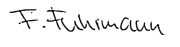
\includegraphics{https://raw.githubusercontent.com/226305Netzwerke/Forschungsbericht-Charles-Manson/master/Unterschriften/Unterschrift-Fuhrmann.PNG}
\textbar{} Name\textbar{} Unterschrift\textbar{}
\textbar--:\textbar--:\textbar{} \textbar{} Frederike
Fuhrmann\textbar{}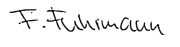
\includegraphics{https://raw.githubusercontent.com/226305Netzwerke/Forschungsbericht-Charles-Manson/master/Unterschriften/Unterschrift-Fuhrmann.PNG}
\textbar{} \textbar{} Eva McGowan\textbar{} \textbar{} \textbar{} Thomas
Nolte\textbar{} \textbar{} \textbar{} Annika Stete\textbar{} \textbar{}
\textbar{} Rromina Trslic\textbar{} \textbar{} \textbar{} Anna
Veyhl\textbar{} \textbar{}

\end{document}
